\documentclass[12pt,a4paper]{report}

% ---------------- Packages ----------------
\usepackage[utf8]{inputenc}
\usepackage[T1]{fontenc}
\usepackage{lmodern}
\usepackage{geometry}
\usepackage{setspace}
\usepackage{graphicx}
\usepackage{hyperref}
\usepackage{longtable}
\usepackage{booktabs}
\usepackage{array}
\usepackage{placeins}
\usepackage{enumitem}
\usepackage{amsmath, amssymb}
\usepackage{float}
\usepackage{caption}
\usepackage{subcaption}
\usepackage{fancyhdr}
\usepackage[backend=biber,style=ieee]{biblatex}
\addbibresource{references.bib}
% Fix biblatex-ieee warning: define missing macro
\providebibmacro{volume+number}{%
  \printfield{volume}%
  \setunit*{\addnbspace}%
  \printfield{number}%
}

\geometry{margin=2.5cm}
\onehalfspacing
\hypersetup{
    colorlinks=true,
    linkcolor=black,
    citecolor=black,
    urlcolor=blue
}

% ---------------- Header / Footer ----------------
\pagestyle{fancy}
\fancyhf{}
\fancyfoot[C]{\thepage}

% ---------------- Document ----------------
\begin{document}

% ---------------- Title Page ----------------
\begin{figure}
    \centering
    
\includegraphics[width=1\linewidth]{uni.png}
    \label{fig:UMALOGO}
\end{figure}

\begin{titlepage}
\centering
{\Large Máster Universitario en Ciberseguridad (2025--2026)}\\[3cm]
{\Large TRABAJO FIN DE MÁSTER }\\[1cm]

{\huge \textbf{Secure Custody Framework for Cryptocurrency Assets (SCFCA)}}\\[2cm]


{\Large Design of a Secure Technical Framework for the Custody, Management, Preservation, and Auditing of Cryptocurrency Assets in Criminal Investigations}\\[2cm]

\textbf{Student:} Lorela Elezaj\\
\textbf{Instructor:} Antonio Maña Gómez \\[2cm]
\vfill
\textbf{Date:} \today

\end{titlepage}

% ---------------- Abstract ----------------
\chapter*{Abstract}
\addcontentsline{toc}{chapter}{Abstract}

This thesis proposes the Secure Custody Framework for Cryptocurrency Assets (SCFCA), a security-oriented reference architecture for the institutional custody, management, preservation, and auditing of cryptocurrency assets seized in criminal investigations. The work is motivated by the operational reality that, unlike traditional financial assets, cryptocurrencies are controlled exclusively through private keys and related authorization mechanisms. In institutional environments, custody therefore becomes a multi-actor governance problem as much as a technical one: a single mistake, lost secret, or unauthorized use of key material can result in irreversible asset loss and can undermine evidentiary integrity.

SCFCA addresses this challenge by defining a custody model centered on explicit trust boundaries, separation of duties, and least-privilege enforcement. The framework structures custody as a controlled lifecycle that includes asset intake and registration, secure key generation and storage, controlled transaction construction and signing, and verifiable oversight suitable for judicial scrutiny. Sensitive custody-impacting actions are mediated through a ticket-based workflow that enforces dual-control approval by independent administrators, preventing unilateral execution and reducing insider-risk concentration. To support accountability and non-repudiation, SCFCA integrates comprehensive event recording and tamper-evident audit logging, enabling later reconstruction of custody decisions, approvals, and execution outcomes. Evidence documentation is treated as a first-class artifact: supporting documents are handled under integrity constraints (e.g., cryptographic hashing) to deter undetected replacement or modification.

The design is derived and validated through a structured threat modeling process based on use cases and misuse scenarios. Rather than relying on generic threat lists, the analysis models how legitimate custody goals can be abused (e.g., unauthorized access, privilege escalation, bypass of dual approval, log tampering, asset record manipulation, document tampering, and data exfiltration) and maps these misuse cases to concrete technical and organizational controls. This approach provides traceability from threats to requirements and from requirements to architectural mechanisms, ensuring that each control in the framework is justified by an explicit risk scenario.

To demonstrate feasibility, the thesis includes a proof-of-concept implementation that operationalizes key SCFCA controls in a prototype custody-management system. The prototype implements server-side role-based access control, case-assignment visibility boundaries, dual-approval ticket workflows, document integrity metadata, and an auditable event trail with integrity protections. While the proof of concept does not execute real blockchain transactions or integrate production hardware custody devices, it validates the governance envelope around key use and shows how approval, execution traceability, and auditability can be enforced in software.

Finally, the work incorporates secure software engineering and DevSecOps-oriented assurance as part of the custody trust story. Because institutional custody platforms are themselves complex software systems built from third-party components, SCFCA treats software supply chain risk as relevant to custody integrity. The proof of concept therefore includes software composition transparency artifacts (e.g., SBOMs and dependency audit evidence) and outlines a dependency governance approach aligned with continuous validation and vulnerability awareness.

Overall, SCFCA contributes a coherent, security-by-design custody framework that integrates governance controls, technical enforcement mechanisms, auditability, and software assurance practices to support reliable institutional handling of seized cryptocurrency assets.

% ---------------- Keywords ----------------
\chapter*{Keywords}
\addcontentsline{toc}{chapter}{Keywords}

Cryptocurrency custody; digital evidence; crypto-asset seizure; institutional custody; judicial custody; forensic investigation;
private-key management; key ceremonies; key generation; key storage; transaction signing; controlled execution;
hot wallets; cold storage; hardware wallets; hardware security module (HSM); multi-signature; threshold signatures; multiparty computation (MPC);
separation of duties; role-based access control (RBAC); least privilege; access management; identity management;
dual control; dual approval; ticket-based workflows; governance workflows; approval traceability;
audit trail; audit reporting; auditability; tamper-evident audit logging; append-only logs; hash chaining; integrity verification;
document integrity; document hashing; SHA-256; evidentiary integrity; chain of custody; non-repudiation; accountability; forensic readiness;
insider threats; external adversary; phishing; credential stuffing; unauthorized access; privilege escalation; IDOR; data exfiltration; denial of service;
threat modeling; misuse cases; attack paths; MITRE ATT\&CK; MITRE D3FEND;
secure software design; security-by-design; trust boundaries; Zero Trust;
DevSecOps; CI/CD security; software supply chain security; dependency governance; vulnerability management;
Software Bill of Materials (SBOM); CycloneDX; Software Composition Analysis (SCA); npm audit; pip-audit; Dependabot;
multi-factor authentication (MFA); re-authentication; session security; CSRF protection; JWT authentication; rate limiting;
FastAPI; SQLAlchemy; Pydantic; bcrypt; WebSockets; React; TypeScript; Vite; TailwindCSS; PostgreSQL; Docker.

% ---------------- TOC ----------------
\tableofcontents
\listoffigures
\listoftables
\clearpage

% =====================================================
\chapter{Introduction}

\section{Context and Motivation}
The rapid development and widespread adoption of cryptocurrencies and digital assets have profoundly transformed the way economic value is created, transferred, and stored. Alongside their legitimate uses, these technologies have increasingly been exploited in a wide range of criminal activities, including financial fraud, money laundering, organized crime, and corruption. As a result, cryptocurrencies have become not only instruments used in criminal operations, but also direct objects of seizure, confiscation, and judicial administration by state authorities.

Law enforcement agencies and judicial institutions are therefore confronted with new operational and technical challenges. Unlike traditional financial assets, cryptocurrencies are not managed through centralized intermediaries such as banks or custodial institutions. Instead, control over these assets depends entirely on cryptographic mechanisms, and more specifically on the secure management of private keys. The loss, compromise, or misuse of these keys can lead to irreversible financial loss and may undermine the integrity of digital evidence relevant to criminal proceedings.

In Albania, these challenges became particularly evident following a significant institutional turning point in 2019 with the establishment of the Special Structure for Anti-Corruption and Organized Crime (SPAK), as part of the broader Justice Reform process. This structure was created to investigate high-level corruption and organized crime, including cases involving senior public officials and individuals with substantial political or economic influence. In the years that followed, these investigations led to the seizure of assets of considerable financial value, including real estate, bank accounts, and other forms of property, among which cryptocurrency assets also began to appear.

At the time, Albania lacked a specific legal framework regulating cryptocurrencies, a situation that reflected a broader absence of technical infrastructure, operational procedures, and institutional experience related to the custody and management of digital assets. This gap exposed a clear misalignment between the increasingly sophisticated techniques employed by criminal organizations and the technical capabilities available to the institutions responsible for combating them. Even as legislative developments concerning cryptocurrencies were introduced in the period 2024–2025, it became evident that legal regulation alone was insufficient to address the underlying technical and organizational challenges.

In practice, the absence of specialized platforms and standardized technical procedures has led to a reliance on ad hoc solutions or international cooperation with foreign institutions possessing more mature technical capabilities in this domain, such as those operating within other European jurisdictions. While such cooperation can provide temporary support, it does not constitute a sustainable or autonomous solution for national authorities tasked with the long-term management and auditing of confiscated digital assets.

This context highlights a fundamental issue: the need for secure, reliable, and auditable technical mechanisms capable of supporting the custody and management of cryptocurrency assets within institutional environments. The challenge is not inherent to blockchain technology itself, but rather to the way custody is implemented through cryptographic controls, access management, role separation, and security processes. Addressing these challenges is essential to ensure the protection of seized assets, maintain institutional accountability, and preserve the integrity of digital evidence throughout the lifecycle of criminal investigations.


\section{Problem Statement}
Despite the growing involvement of cryptocurrencies in criminal investigations and asset confiscation procedures, state institutions continue to face significant technical and organizational shortcomings in the secure custody and management of seized digital assets. While recent legislative developments have begun to address the legal status of cryptocurrencies, they do not resolve the practical challenges associated with their technical custody, control, and auditability.

Cryptocurrency assets differ fundamentally from traditional financial assets in that ownership and control are determined exclusively by cryptographic private keys. The absence of secure and well-defined mechanisms for private key management exposes confiscated assets to critical risks, including irreversible loss, unauthorized access, and misuse. These risks are further amplified in institutional environments where multiple actors are involved, and where inadequate separation of duties or poorly defined access controls may enable insider threats or abuse of privileges.

In many existing institutional contexts, there is no standardized technical framework governing how confiscated cryptocurrency assets should be registered, stored, accessed, transferred, or audited. Custody procedures are often handled in an ad hoc manner, relying on fragmented tools, manual processes, or external entities. Such approaches lack transparency, are difficult to audit, and do not provide sufficient guarantees of integrity, non-repudiation, or traceability throughout the lifecycle of the assets.

Furthermore, the absence of tamper-evident audit mechanisms and clearly defined role-based responsibilities undermines institutional accountability. Without comprehensive and verifiable audit trails, it becomes difficult to demonstrate that assets have been managed in accordance with legal and procedural requirements, or to reliably attribute actions to specific authorized actors. This represents a critical weakness in contexts where digital assets may constitute both financial value and evidentiary material in ongoing judicial proceedings.

Consequently, the core problem addressed in this work is not the regulation of cryptocurrencies as financial instruments, nor the operation of blockchain networks themselves, but rather the lack of a secure, standardized, and auditable technical framework for the institutional custody and management of confiscated cryptocurrency assets. Addressing this problem requires a systematic approach that integrates cryptographic controls, access management, role separation, and auditability into a coherent custody model suitable for use by state authorities.


\section{Objectives}
The objective of this Master’s Thesis is to design a secure technical framework for the custody, management, preservation, and auditing of cryptocurrency assets within the context of criminal investigations. The work focuses on addressing the technical and cybersecurity challenges associated with the institutional management of confiscated crypto-assets, proposing an architecture capable of mitigating both external and internal threats, ensuring the integrity and availability of assets, and guaranteeing the traceability and auditability of all operations performed.

The proposed framework, referred to as the Secure Custody Framework for Cryptocurrency Assets (SCFCA), is conceived as a technology-agnostic solution intended for use by public authorities or authorized entities responsible for the judicial custody of cryptocurrency assets. The scope of this work does not focus on the development of blockchain technologies themselves, but rather on the design of security mechanisms, cryptographic management, access control, separation of duties, and auditing processes that enable secure and verifiable asset custody in institutional environments.

\subsection{General Objective}
\begin{itemize}
\item Design a reference technical framework that enables public institutions to implement secure,  auditable and resilient systems for the custody, management, preservation, and auditing of cryptocurrency assets in the context of criminal investigations.
\end{itemize}

\subsection{Specific Objectives}
\begin{itemize}
 \item To analyze the technical characteristics and security risks associated with the institutional custody of cryptocurrencies, with particular emphasis on cryptographic key management and internal and external threats.
 \item To identify and model the relevant threats affecting institutional cryptocurrency custody systems through structured threat analysis and misuse scenario modeling, and to map these threats to appropriate security controls.
\item To define a secure custody architecture based on security-by-design principles, separation of duties, access control, and role management.
To propose technical mechanisms for preserving the integrity and availability of cryptocurrency assets, as well as for the controlled execution and validation of institutional transfers.
\item To design a logging and auditing system that guarantees traceability, non-repudiation, and accountability for all operations performed on the assets.
To align the proposed framework with European cybersecurity, governance, and risk management standards and best practices, ensuring its applicability within an institutional European context.
\end{itemize}



% =====================================================
\chapter{State of the Art}

\section{Cryptocurrency Custody Models}
The custody of cryptocurrency assets refers to the mechanisms and processes through which private cryptographic keys are generated, stored, protected, and ultimately used to authorize transactions on blockchain networks. In contrast to traditional financial assets, which are typically managed by centralized intermediaries such as banks or financial institutions, cryptocurrencies operate within decentralized infrastructures. In these environments, ownership and control are defined solely by possession of the corresponding private keys. Whoever controls the key controls the asset.\cite{FintechNews}

For this reason, custody models are not merely technical implementations; they directly determine the security, availability, and long-term integrity of digital assets. The design of a custody solution therefore reflects underlying assumptions about trust, risk tolerance, and operational requirements.

Over time, several custody models have emerged in practice, each shaped by different security priorities and usage scenarios. These models are commonly distinguished according to the degree of control retained by the asset holder and the mechanisms adopted to protect private keys. While some approaches prioritize accessibility and operational efficiency, others emphasize isolation and strict protection against unauthorized access. The balance between these dimensions defines the practical trade-offs of each custody model.

\subsection{Hot Wallet Custody}

Hot wallets are custody solutions in which private keys are stored in environments connected to the internet. They are typically used to enable frequent, automated, or near-instant transactions, making them particularly attractive for exchanges, payment platforms, and services that require continuous operational availability.

The main advantage of hot wallets lies in their accessibility. Because the signing infrastructure is online, transactions can be processed quickly and with minimal manual intervention. In commercial settings, this responsiveness is often considered essential.

However, this accessibility introduces a significant security trade-off. Internet connectivity inevitably expands the attack surface. Private keys stored in hot environments may be exposed to malware, exploitation of software vulnerabilities, phishing campaigns targeting privileged users, or unauthorized access to backend systems. Even when advanced security controls are implemented, the residual risk associated with constant network exposure cannot be fully eliminated.

From an institutional perspective—particularly in contexts involving seized or confiscated assets—the use of hot wallets without additional protective layers is difficult to justify. Judicial custody environments typically prioritize integrity, auditability, and resilience over transactional speed. For high-value or legally sensitive assets, the operational convenience of hot storage must therefore be carefully weighed against the elevated risk profile it entails.

\subsection{Cold Storage Custody}

Cold storage refers to custody models in which private keys are generated and stored in environments that remain offline and isolated from network connectivity. By removing direct exposure to the internet, this approach significantly reduces the risk of remote compromise and is widely regarded as one of the most secure methods for protecting cryptocurrency assets.

Cold storage can take different forms, including hardware devices, air-gapped computers, or dedicated systems used exclusively for signing operations. In all cases, the underlying objective is the same: to minimize the attack surface by limiting external access to cryptographic material.

The security benefits of cold storage are substantial, particularly in scenarios where asset preservation is the primary concern. However, this increased protection comes at an operational cost. Transaction authorization typically requires physical access to secure environments, coordinated procedures, and manual validation steps. As a result, execution times may be slower and workflows less flexible compared to online custody solutions.

In institutional settings, especially those involving judicial custody, cold storage is often considered appropriate for long-term asset preservation. Nevertheless, it may not fully address the need for structured approval workflows, traceability mechanisms, and controlled governance processes. While it strengthens cryptographic protection, it does not, by itself, solve organizational or accountability challenges.

\subsection{Custodial Services and Centralized Custody}

Centralized custodial services provide custody on behalf of users by managing private keys within controlled infrastructures. In this model, users relinquish direct control over cryptographic material and rely on the custodian to implement security mechanisms, operational safeguards, and compliance procedures. This approach is common among regulated exchanges and specialized institutional custody providers.

From a technical point of view, centralized custody concentrates both responsibility and risk within a single organizational boundary. Analyses of major cryptocurrency fraud cases and exchange collapses demonstrate that many large-scale losses have resulted not from weaknesses in blockchain protocols, but from failures in centralized custody infrastructures \cite{Scharfman2024}. When private keys are aggregated and managed within a single system, that system becomes a high-value target.

The security of centralized custody therefore depends less on blockchain resilience and more on internal governance, infrastructure hardening, access control enforcement, and operational discipline. As emphasized in modern cryptographic security literature, control over key material ultimately defines control over assets \cite{Aumasson2021}. The trust boundary shifts from protocol-level guarantees to institutional safeguards. Furthermore, infrastructure security practices highlight that centralization increases systemic risk concentration, requiring strict operational controls and monitoring \cite{Vehent2018}.

In institutional contexts involving confiscated assets, reliance on external custodians introduces additional concerns. Questions of jurisdiction, accountability, audit transparency, and long-term autonomy become central. While professional custodians may implement advanced security controls, delegating custody to third parties can complicate evidentiary integrity and institutional responsibility, particularly in judicial environments where traceability and non-repudiation are essential.

\subsection{Hardware-Based Custody}

Hardware-based custody models rely on dedicated devices specifically designed to generate, store, and use cryptographic keys in a secure manner. Unlike purely software-based solutions, these devices isolate key material within protected hardware environments, reducing the risk of extraction through conventional malware or remote compromise.

Common examples include hardware wallets and Hardware Security Modules (HSMs). These devices are engineered to resist physical tampering and unauthorized key access. In many enterprise environments, HSMs are used to enforce strict cryptographic policies, including controlled key generation, secure key storage, and regulated signing operations. By embedding security mechanisms at the hardware level, such systems provide stronger guarantees than general-purpose computing platforms.

The primary advantage of hardware-based custody lies in its ability to enforce security boundaries independently of the host system. Even if the surrounding infrastructure is partially compromised, properly configured hardware devices can prevent direct exposure of private keys. This architectural separation significantly strengthens key protection in institutional contexts.

However, hardware-based custody does not eliminate governance risks. The security of the system still depends on access control configuration, role assignment, and operational procedures. If excessive privileges are granted or physical access controls are poorly implemented, the intended security benefits may be weakened. In multi-actor institutional environments, hardware protection must therefore be complemented by structured approval workflows, audit logging, and separation-of-duties mechanisms.

For these reasons, hardware-based custody is widely adopted in governmental and enterprise settings, but its effectiveness ultimately depends on the broader security architecture in which it is embedded.


\section{Digital Asset Governance}

Digital asset governance encompasses the organizational structures, policies, procedures, and technical controls through which digital assets are managed, monitored, and controlled within an institution. In the context of cryptocurrencies, governance extends beyond traditional financial oversight to include cryptographic key management, access control enforcement, accountability mechanisms, and auditability throughout the asset lifecycle.

In institutional environments—particularly those involving law enforcement or judicial authorities—governance is not merely an operational concern but a legal and regulatory necessity. The handling of seized or confiscated cryptocurrency assets must comply with principles of accountability, traceability, and procedural integrity. Actions performed on digital assets may carry legal consequences and evidentiary relevance, which places additional requirements on custody infrastructures.

Within the European regulatory landscape, the governance of crypto-assets has gained increasing formalization. The Markets in Crypto-Assets Regulation (MiCA) \cite{MiCA2023} establishes a harmonized framework for the issuance, custody, and supervision of crypto-assets across the European Union. While MiCA primarily addresses market actors and service providers, its emphasis on transparency, operational responsibility, and supervisory oversight reinforces the necessity of structured custody governance mechanisms. Institutions managing digital assets must therefore demonstrate internal controls, clear allocation of responsibilities, and reliable record-keeping practices.

In parallel, the Digital Operational Resilience Act (DORA) \cite{DORA2022} strengthens requirements for ICT risk management, incident reporting, and operational resilience within financial entities. Although not limited to cryptocurrency services, DORA highlights the importance of infrastructure hardening, monitoring, and continuity planning in systems handling sensitive financial operations. These regulatory developments underscore that digital asset custody cannot rely solely on cryptographic protection; it must also embed resilience and risk management at the architectural level.

A central governance challenge arises from the decentralized nature of blockchain systems. While blockchain networks provide immutability and public verifiability at the ledger level, these guarantees do not extend to off-chain custody processes. Decisions regarding key access, transaction authorization, and workflow approval occur within institutional environments and remain dependent on internal procedures. Governance failures at this layer can undermine the integrity of asset management, regardless of the robustness of the underlying blockchain protocol.

Another critical dimension is auditability. Effective governance requires comprehensive, tamper-evident audit trails capable of linking authorized actors, approved workflows, and executed transactions. Without verifiable logging and non-repudiation mechanisms, institutions may be unable to reconstruct events, demonstrate compliance, or defend the integrity of seized assets in judicial proceedings.

In practice, digital asset governance is therefore inseparable from technical design. Regulatory principles such as least privilege, separation of duties, and operational resilience must be concretely implemented through access control models, approval workflows, logging mechanisms, and infrastructure safeguards. A custody system that fails to integrate these elements risks not only security compromise but also regulatory and institutional non-compliance.

\section{Security Threats in Custody Systems}

Cryptocurrency custody systems are exposed to a broad spectrum of security risks that stem from the fundamental properties of blockchain-based assets. Unlike traditional financial infrastructures, where transactions can often be reversed and institutional controls mediate ownership, cryptocurrency systems rely entirely on cryptographic key control. If a private key is compromised or misused, the resulting asset transfer is typically irreversible. This characteristic makes custody security not merely important, but critical.

External attacks remain one of the most visible threat categories. Over the past decade, several high-profile exchange breaches have demonstrated how vulnerabilities in hot wallet infrastructure, backend systems, or access management mechanisms can result in massive asset losses. Incidents such as the Mt. Gox collapse in 2014 and subsequent large-scale exchange hacks illustrate how insufficient key segregation, inadequate monitoring, and weak internal controls can lead to catastrophic consequences. These events highlight that internet-facing custody components significantly increase the attack surface and must be carefully isolated or minimized.

However, external attacks represent only part of the threat landscape. Insider threats often pose a more subtle and complex risk. Individuals with legitimate system access may abuse privileges, bypass procedural safeguards, or exploit weak separation-of-duties controls. In environments where approval workflows are poorly enforced or logging mechanisms are insufficient, malicious or negligent insiders may initiate unauthorized transfers or manipulate records without immediate detection. Institutional custody systems, especially those involving confiscated assets, are particularly sensitive to such risks because of the legal and reputational implications involved.

Key management failures constitute another critical threat category. Private keys may be improperly generated, inadequately protected, insufficiently backed up, or mishandled during operational procedures. Unlike passwords or traditional credentials, lost or compromised cryptographic keys cannot be reset. Several custody failures in the industry have stemmed not from sophisticated attacks, but from poor operational practices, inadequate redundancy, or unclear governance structures around key access.

Audit and traceability weaknesses further compound these risks. In some historical cases, institutions and exchanges were unable to reconstruct transaction histories or determine responsibility due to incomplete or manipulable logs. Without tamper-evident logging and non-repudiation mechanisms, organizations may struggle to demonstrate procedural compliance or defend against accusations of mismanagement. For systems handling judicially seized assets, such deficiencies could undermine evidentiary integrity in court proceedings.

Finally, organizational and governance failures frequently amplify technical vulnerabilities. The collapse of certain centralized crypto entities has shown that weak internal governance, lack of independent oversight, and concentration of authority can be as damaging as external cyberattacks. The FTX crisis, for example, underscored how governance breakdowns and insufficient internal controls may lead to severe financial and institutional consequences, even in the absence of purely technical compromise.

Taken together, these incidents demonstrate that cryptocurrency custody risks are multidimensional. They encompass technical vulnerabilities, insider misuse, operational failures, and governance deficiencies. Effective custody design therefore requires a holistic approach that integrates cryptographic protection, structured approval mechanisms, role separation, tamper-evident logging, and institutional accountability into a coherent architectural framework. The understanding of these threat categories provides the foundation for the threat modeling and security requirements defined in subsequent chapters.

\section{Gap Analysis}

The review of existing custody models, governance approaches, and security threats reveals a clear mismatch between current industry practices and the specific requirements of institutional environments responsible for managing confiscated cryptocurrency assets.

Most existing custody solutions have been designed for commercial use cases. Exchanges and private custodians typically prioritize liquidity, operational efficiency, and customer-facing services. While many of these platforms implement advanced security mechanisms, their architectural priorities differ fundamentally from those of law enforcement or judicial institutions. In commercial settings, availability and transaction throughput are often emphasized; in institutional custody of seized assets, traceability, procedural integrity, and accountability are equally — if not more — critical.

Hot wallet solutions, for example, provide operational flexibility but expose assets to higher levels of external risk. Cold storage, on the other hand, offers strong protection against remote attacks but does not inherently provide structured multi-actor governance or formalized approval workflows. Hardware-based solutions strengthen key protection, yet they do not automatically enforce institutional separation of duties or prevent misuse of privileged access. In practice, technical safeguards and governance mechanisms are frequently treated as separate concerns rather than as components of a unified framework.

Centralized custodial services introduce an additional layer of dependency. When institutions rely on third-party providers, questions arise regarding jurisdiction, supervisory control, evidentiary responsibility, and long-term autonomy. For confiscated assets that may be subject to legal disputes or court proceedings, such dependencies can complicate accountability and procedural transparency.

Another significant gap lies in the integration of auditability within custody systems. Although blockchain transactions are inherently transparent at the ledger level, institutional decisions—such as who authorized a transfer, under what approval conditions, and through which internal workflow—remain off-chain. Existing solutions rarely provide a structured, tamper-evident linkage between institutional authorization processes and executed blockchain transactions. This disconnect weakens the ability of institutions to demonstrate procedural compliance and reconstruct decision histories.

Furthermore, regulatory developments within the European Union, including MiCA and DORA, emphasize operational resilience, internal controls, and risk management. However, there remains no standardized technical framework specifically tailored to the institutional custody of seized crypto-assets. Institutions often rely on ad hoc combinations of tools, manual procedures, or externally managed solutions, leading to inconsistencies and potential governance weaknesses.

In summary, the current landscape lacks an integrated, security-oriented technical framework designed specifically for institutional custody in criminal investigation contexts. Existing models address isolated aspects of security or governance but do not systematically combine cryptographic protection, structured approval workflows, separation of duties, tamper-evident logging, and regulatory alignment within a single coherent architecture. 

This gap motivates the development of the Secure Custody Framework for Cryptocurrency Assets (SCFCA), which seeks to formalize and integrate these elements into a structured, institution-oriented custody model.

Existing gap analyses for institutional cryptocurrency custody usually focus on governance, key control, and auditability, but they pay less attention to the software supply chain dimension of secure system construction. This is a relevant omission because institutional custody platforms are themselves modern software systems composed of dependencies, frameworks, containers, and build pipelines. A technically secure custody design that ignores dependency trust, build integrity, and software component transparency remains incomplete. For this reason, the gap addressed by SCFCA is both architectural and supply-chain related: the need for an institutional custody framework that combines governance controls with secure software engineering and DevSecOps-oriented assurance.

\section{European Regulatory Context for Crypto-Asset Custody}

The regulatory environment surrounding crypto-assets in the European Union has evolved significantly in recent years. Although early cryptocurrency activity operated in largely unregulated spaces, the European legislator has progressively introduced structured frameworks aimed at enhancing transparency, accountability, and operational resilience in digital asset markets.

A major development in this context is the Markets in Crypto-Assets Regulation (MiCA) \cite{MiCA2023}. MiCA establishes a harmonized regulatory framework governing the issuance, offering, and custody of crypto-assets within the European Union. Although its primary focus lies on crypto-asset service providers and market participants, MiCA emphasizes principles that are directly relevant to institutional custody systems, including operational responsibility, safeguarding of client assets, governance transparency, and supervisory oversight.

In parallel, the Digital Operational Resilience Act (DORA) \cite{DORA2022} introduces strengthened requirements for ICT risk management, incident reporting, third-party risk control, and operational continuity across financial entities. DORA reflects a broader recognition that digital infrastructures handling financial assets must demonstrate resilience against cyber threats, internal misuse, and systemic disruptions. Even where institutional custody falls outside strict financial market regulation, the resilience principles embedded in DORA provide a strong reference point for high-assurance system design.

These regulatory developments share a common emphasis on internal controls, separation of responsibilities, traceability of actions, and continuous monitoring. Importantly, they highlight that governance and security are not abstract compliance concepts but architectural requirements. Systems managing crypto-assets must be designed in a manner that enables institutions to demonstrate control over access, authorization workflows, and incident handling procedures.

For institutions involved in criminal investigations and asset confiscation, regulatory alignment carries additional significance. Beyond safeguarding economic value, custody systems must preserve evidentiary integrity, support judicial scrutiny, and withstand external audit. The European regulatory framework therefore reinforces the necessity of embedding structured governance and operational resilience directly into the technical architecture of custody systems.

This regulatory context provides a foundational backdrop for the development of the Secure Custody Framework for Cryptocurrency Assets (SCFCA), which seeks to operationalize governance principles through concrete architectural mechanisms.

\section{Software Supply Chain Security and Dependency Trust in Modern Systems}
Modern secure systems are not built solely from custom code. They are assembled from frameworks, libraries, runtimes, container images, operating system packages, and external services. As a result, the security of a software system depends not only on its business logic, but also on the trustworthiness of the components on which it relies.

This issue is particularly important in contemporary software engineering because dependency relationships have become deep and difficult to inspect manually. A project may include a limited number of direct dependencies while indirectly incorporating a much larger number of transitive dependencies. Each of these components may introduce vulnerabilities, licensing constraints, maintenance risks, or trust concerns. The practical consequence is that software development increasingly operates within a software supply chain rather than a closed implementation boundary.

For security-sensitive institutional systems, this has direct architectural implications. External components cannot be treated as fully trusted by default. Their integration must be governed by explicit trust assumptions, provenance awareness, vulnerability analysis, and update discipline. In practice, this means minimizing unnecessary dependencies, preferring well-maintained components, isolating sensitive functions, and continuously monitoring the software composition of the system.

Software Bill of Materials (SBOM) practices emerge in this context as a transparency mechanism. An SBOM provides a structured inventory of the software components included in a system, including versions, origins, and dependency relationships. In security-oriented environments, SBOMs support vulnerability management, change impact analysis, regulatory reporting, and software supply chain traceability. They do not guarantee security by themselves, but they improve visibility and make dependency risk manageable.

Closely related to SBOM practices is Software Composition Analysis (SCA), which enables automated identification of dependencies and correlation with known vulnerabilities. In DevSecOps environments, SCA and SBOM generation are increasingly integrated into CI/CD pipelines so that dependency risk is evaluated continuously rather than only at release time. This shift is especially relevant to institutional platforms where evidentiary integrity, auditability, and operational continuity are critical.

For the SCFCA context, software supply chain security is not a secondary implementation concern. A compromise in a third-party component, build script, container image, or dependency chain could affect authentication, ticket execution, audit logging, or document integrity. Consequently, the design and evaluation of a secure custody framework must extend beyond role models and workflows to include dependency governance, build integrity, and software composition transparency.
% =====================================================
\chapter{Methodology}

\section{Methodological Foundations}

This thesis adopts a design-oriented security engineering methodology grounded in secure software design, security patterns, misuse-case analysis, and traceable security-by-design principles. The work is not driven by coding first; it is driven by security requirements, institutional constraints, and verifiable design decisions. This methodological position is consistent with security engineering approaches that integrate security concerns into system design from the earliest stages rather than treating them as late implementation additions~\cite{Schumacher2006,Fluchs2021}.

The methodology follows a model-driven approach inspired by Secure Tropos and structured requirement derivation, with the goal of producing a traceable security architecture for institutional cryptocurrency custody. In particular, the methodology emphasizes:

\begin{itemize}
    \item Integrating security constraints from the earliest design stages
    \item Modeling institutional actors, goals, and dependencies explicitly
    \item Capturing abuse and failure conditions through misuse scenarios
    \item Deriving security requirements systematically from identified risks
    \item Maintaining traceability between threats, requirements, and architectural controls
\end{itemize}

The output of this chapter is therefore a set of engineering artifacts (models, requirements, and traceability links) that support the architectural design and the proof-of-concept validation presented in later chapters.

\section{SCFCA as an ISO/IEC 27001-Aligned ISMS}

SCFCA is conceived as a domain-specific Information Security Management System (ISMS) focused on the secure custody, management, preservation, and audit of cryptocurrency assets in criminal investigations. This positioning connects the framework with the logic of ISO/IEC 27001, where information security is managed through a structured, risk-based, and continuously improved system rather than through isolated technical controls.

The control perspective is also informed by ISO/IEC 27002 and NIST SP 800-53, which provide structured catalogues of security controls relevant to access control, auditability, operational security, and monitoring~\cite{ISO27001,ISO27002,NIST80053}.

In this thesis, SCFCA does not claim to implement a complete certifiable ISO/IEC 27001 ISMS for a real organization. Such a claim would require an organizational audit scope, a formal Statement of Applicability, complete operational procedures, management review, internal audit evidence, and certification-oriented documentation. Instead, SCFCA adopts the ISMS logic as a methodological foundation for structuring the custody scope, security objectives, risk treatment, control implementation, monitoring, evaluation, and improvement of a secure cryptocurrency custody framework.

The continuous improvement logic of SCFCA follows the Plan--Do--Check--Act (PDCA) model. The \textit{Plan} phase defines the custody scope, institutional actors, protected assets, risks, security objectives, and legal or evidentiary constraints. The \textit{Do} phase corresponds to the implementation of the proposed security controls and workflows, including role-based access control, dual approval, ticketing, immutable records, document hashing, and audit logging. The \textit{Check} phase evaluates whether these controls operate effectively through documented monitoring, measurement, analysis, and evaluation criteria. Finally, the \textit{Act} phase introduces corrective actions and improvements based on audit findings, detected weaknesses, incidents, or changes in the institutional context.

\begin{figure}[ht]
    \centering
    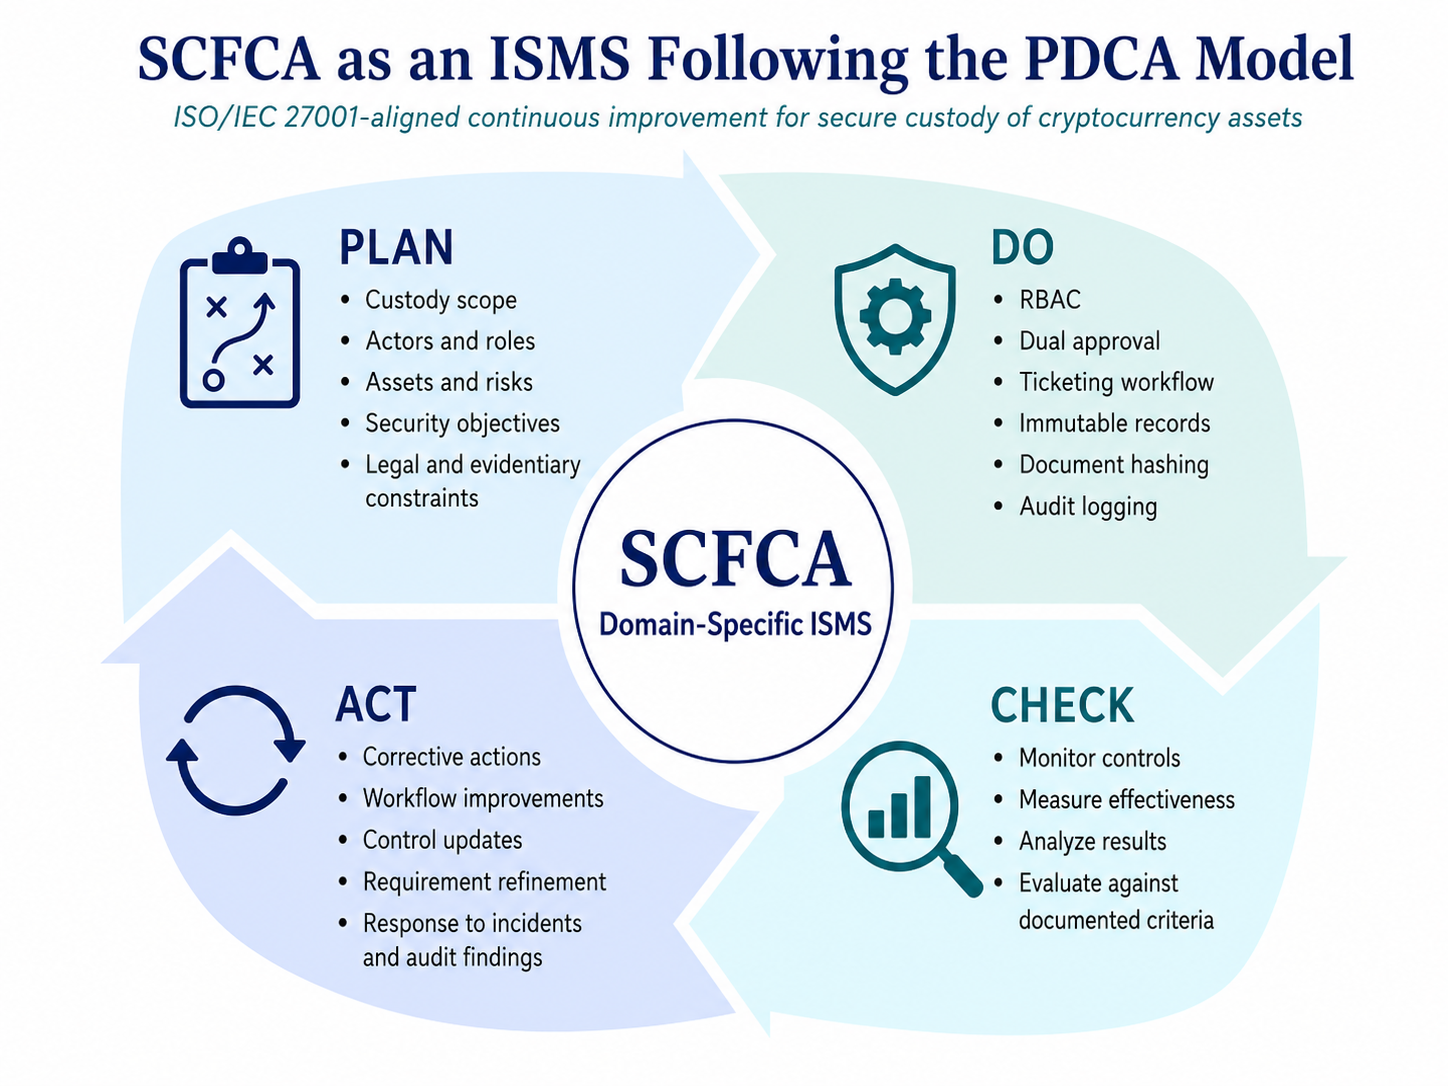
\includegraphics[width=0.95\textwidth]{figure11.png}
    \caption{SCFCA as an ISO/IEC 27001-aligned ISMS following the PDCA continuous improvement model.}
    \label{fig:scfca-pdca-isms}
\end{figure}

The effectiveness of SCFCA is therefore not assumed by design. It must be evaluated through defined and documented monitoring, measurement, analysis, and evaluation criteria. Examples of such criteria include the correct enforcement of access restrictions, prevention of unauthorized custody actions, verification that sensitive operations require dual administrative approval, preservation of immutable asset records, integrity validation of uploaded documents, completeness of audit events, and traceability from custody request to approval, execution, and audit review.

This positioning is important because the custody of seized cryptocurrency assets is both a technical and institutional security problem. Technical mechanisms such as hashing, authentication, authorization, and audit logging are necessary, but they are not sufficient on their own. They must be embedded within a management structure that defines responsibilities, separates duties, monitors effectiveness, and supports continuous improvement.

For this reason, the SCFCA methodology combines ISO/IEC 27001-aligned ISMS thinking with security-by-design and model-driven engineering. ISO/IEC 27001 provides the management-system logic, PDCA provides the continuous improvement cycle, and the model-driven security engineering process provides the concrete mechanism for deriving threats, requirements, controls, architecture, and validation evidence.

\section{Security-by-Design and Model-Driven Engineering}
This research follows a security-by-design principle for developing the Secure Custody Framework for Cryptocurrency Assets (SCFCA). The objective is not to deliver a production-ready custody platform, but to design and justify a secure reference architecture suitable for institutional custody in criminal investigations, where auditability, role accountability, and tamper resistance are mandatory.
Security requirements are treated as primary design drivers from the start. The framework is therefore modeled to explicitly address realistic threats such as insider abuse, privilege escalation, unauthorized key usage, custody manipulation, and audit log tampering.

The SCFCA is developed using a top-down, model-driven process that consists of:

\begin{enumerate}
    \item \textbf{Institutional context and actor modeling:} definition of roles, responsibilities, trust assumptions, and separation of duties.
    \item \textbf{Threat identification through misuse scenarios:} modeling how legitimate goals can be abused or bypassed by malicious actors.
    \item \textbf{Requirement derivation:} specification of functional requirements and the corresponding security and non-functional requirements derived from threats and governance constraints.
    \item \textbf{Architectural refinement:} transformation of requirements into architectural components and enforceable controls (e.g., RBAC, dual control, immutable logging).
    \item \textbf{Traceability management:} maintaining explicit links from threats to requirements and from requirements to architectural decisions.
\end{enumerate}

This workflow ensures that security controls are not introduced as ad hoc features, but as traceable design decisions derived from identified threats, requirements, and architectural constraints~\cite{Schumacher2006,Fluchs2021}.Each control included in the architecture must be justified by a specific threat scenario and mapped to a corresponding requirement, enabling systematic review and later validation.

\section{Threat Analysis Based on Use Cases and Misuse Scenarios}

Threat analysis in this thesis is performed using a misuse-case--driven approach integrated with goal-oriented modeling. Instead of relying only on generic threat taxonomies, threats are identified by analyzing how legitimate custody goals can be disrupted, abused, or bypassed in the SCFCA context. This approach is supported by misuse-case literature, where malicious goals are modeled explicitly in order to derive security requirements from adversarial behavior~\cite{Sindre2001,Choi2006}.

The analysis distinguishes between two categories of actors:

\begin{itemize}
    \item \textbf{Legitimate institutional actors:} Case Handler, Administrator, and Auditor.
    \item \textbf{Adversarial actors:} External Adversary and Malicious Insider.
\end{itemize}

For each legitimate operational goal (e.g., intake of seized assets, controlled access to wallets, authorization of transfers, and generation of audit evidence), one or more misuse scenarios are defined. These misuse cases represent concrete adversarial objectives such as unauthorized access to custody material, privilege escalation, manipulation of custody actions, audit log tampering, repudiation attempts, and data exfiltration.

Each misuse case is analyzed using the following structure:

\begin{enumerate}
    \item \textbf{Malicious goal:} what the adversary attempts to achieve.
    \item \textbf{Attack path:} how the adversary could realistically pursue the goal within the system and organizational workflow.
    \item \textbf{Mitigation and controls:} security mechanisms that prevent, detect, or limit the impact of the misuse case.
\end{enumerate}

This produces an explicit traceability chain that is maintained throughout the design:

\begin{center}
\textit{Misuse Case} $\rightarrow$ \textit{Threatened Goal} $\rightarrow$ \textit{Security Control} $\rightarrow$ \textit{Formal Requirement}
\end{center}

By linking misuse cases directly to institutional workflows (such as dual-control authorization, separation of duties, and tamper-evident audit logging), the threat analysis avoids abstract threat lists and instead drives concrete requirement derivation. The resulting output of this phase is a structured set of threats and mitigations that directly informs both the requirement specification and the architectural controls defined later in the thesis.

The threat analysis is performed in the following steps:

\begin{enumerate}
    \item Identification of critical assets and custody goals.
    \item Identification of actors, trust assumptions, and adversary capabilities.
    \item Definition of misuse cases targeting specific goals and custody operations.
    \item Mapping of misuse cases to candidate controls (preventive and detective).
    \item Formalization of selected controls as security requirements.
\end{enumerate}

This approach supports defense-in-depth by combining governance mechanisms (dual control and accountability) with technical controls (authentication, authorization, tamper-evident logging, and monitoring), ensuring that security requirements are justified by explicit and realistic risk scenarios.

\section{Model-Driven Architectural Development}

The SCFCA architecture is developed through a model-driven security engineering process. Visual models define the system boundary, institutional actors, trust assumptions, security requirements, and architectural controls before the proof-of-concept implementation is developed. This ensures that design decisions are traceable and that the architecture is aligned with the threat model rather than derived from implementation convenience.
This traceability-oriented view is consistent with security-by-design approaches that link functions, threats, controls, and design decisions into an explicit assurance chain~\cite{Fluchs2021}.

The development workflow uses the following toolchain:

\begin{itemize}
    \item \textbf{Visual Paradigm:} creation of requirements, Secure Tropos, and UML models.
    \item \textbf{Secure Tropos / goal-oriented modeling:} representation of actor goals, dependencies, misuse scenarios, and security constraints.
    \item \textbf{UML diagrams:} use case, component, sequence, activity, and deployment diagrams.
    \item \textbf{PlantUML:} text-based diagram representation for reproducibility and version control.
    \item \textbf{GitLab/GitHub:} version control for thesis sources, diagrams, traceability artifacts, and proof-of-concept code.

\paragraph{Repository hosting strategy.}
The SCFCA repository is maintained in both GitLab and GitHub. GitLab is used as the main DevSecOps and traceability platform for CI/CD validation, while GitHub is kept as a synchronized mirror because it integrates directly with Overleaf for the LaTeX thesis workflow.

    \item \textbf{Visual Studio / Visual Studio Code:} implementation and validation of the proof-of-concept prototype.
\end{itemize}

\subsection{Modeling Phase}

The modeling phase transforms the institutional custody problem into explicit models that guide the architecture and the proof of concept. Artifacts include actor models, use case and misuse case diagrams, Secure Tropos goal models, requirements models, domain and domain security models, and activity and sequence diagrams for key custody workflows. These models make security assumptions explicit: separation of duties, dual approval, restricted access, document integrity, and tamper-evident auditability are embedded into the system design rather than left as informal procedural rules.

\begin{figure}[ht]
    \centering
    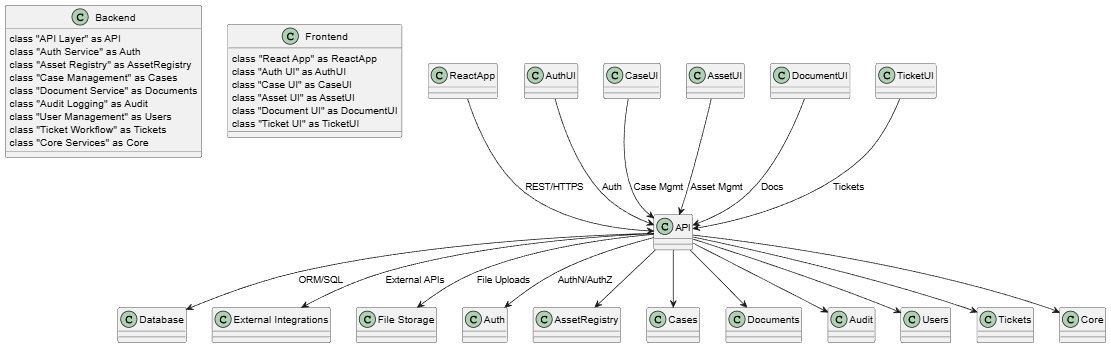
\includegraphics[width=\textwidth]{docs/architecture/architecture-highlevel.png}
    \caption{High-level system/component architecture of the SCFCA project.}
    \label{fig:highlevel-architecture}
\end{figure}

\subsection{Requirement-to-Architecture Traceability}

Traceability connects the threat analysis with the architectural design. The chain followed throughout this thesis is:

\[
\text{Misuse Case} \rightarrow \text{Security Requirement} \rightarrow
\text{Architectural Control} \rightarrow \text{Validation Evidence}
\]

For example, the dual-approval workflow is derived from misuse scenarios involving unauthorized custody execution, while tamper-evident audit logs are derived from scenarios involving log modification or deletion.

\subsection{Repository and Version Control}

Project artifacts are managed through version control to support reproducibility and controlled evolution. The repository contains thesis source files, exported Visual Paradigm diagrams, traceability artifacts, proof-of-concept source code, tests, and configuration files.

\subsection{Proof-of-Concept Implementation}

A proof-of-concept prototype validates the feasibility of the main security controls defined in the architecture. The PoC is not a complete production custody platform; its purpose is to demonstrate that the most important security properties can be enforced in software, specifically: role-based access control and least-privilege enforcement, separation of duties between Case Handler, Administrator, and Auditor, dual-administrator approval for custody-impacting actions, document integrity verification through cryptographic hashing, and tamper-evident audit logging.

\subsection{Architectural Refinement}

The architecture is refined iteratively. When requirements, misuse cases, or implementation constraints reveal inconsistencies, the affected models and controls are updated to preserve least privilege, separation of duties, dual approval, immutable evidence records, and audit integrity.

\section{Validation and Proof-of-Concept Strategy}

The validation strategy checks whether the proposed architecture is internally consistent and whether its most critical security controls can be implemented in practice. It is design-oriented: it does not attempt to prove production readiness, but to show that the security requirements are enforceable within the defined scope of the thesis.

Validation is performed through three complementary activities: review of Visual Paradigm models for consistency between actors, goals, requirements, and workflows; verification of traceability between misuse cases, requirements, architectural controls, and PoC evidence; and testing of the prototype to confirm selected security properties, especially access control, dual approval, document hashing, and audit logging.

\subsection{Model Consistency Validation}

Model consistency is checked in Visual Paradigm by reviewing whether the diagrams describe a coherent system. The focus is on actor responsibilities, system boundaries, security assumptions, misuse scenarios, and the architectural components enforcing the main requirements. This step detects contradictions such as actors with excessive privileges, security requirements without a corresponding control, or workflows that bypass the intended approval process.

\subsection{Requirement Traceability Verification}

Traceability verification confirms that the main threats are connected to specific requirements and controls. For example, privilege escalation is linked to least-privilege enforcement and controlled role assignment; document tampering is linked to PDF-only uploads and SHA-256 integrity verification.

\subsection{Proof-of-Concept Implementation Validation}

The PoC is validated by testing whether the prototype enforces the security constraints defined in the architecture: role restrictions and server-side authorization checks, prevention of custody execution without required approvals, generation of audit events for relevant workflow actions, and preservation of document and asset integrity constraints.

\begin{figure}[ht]
    \centering
    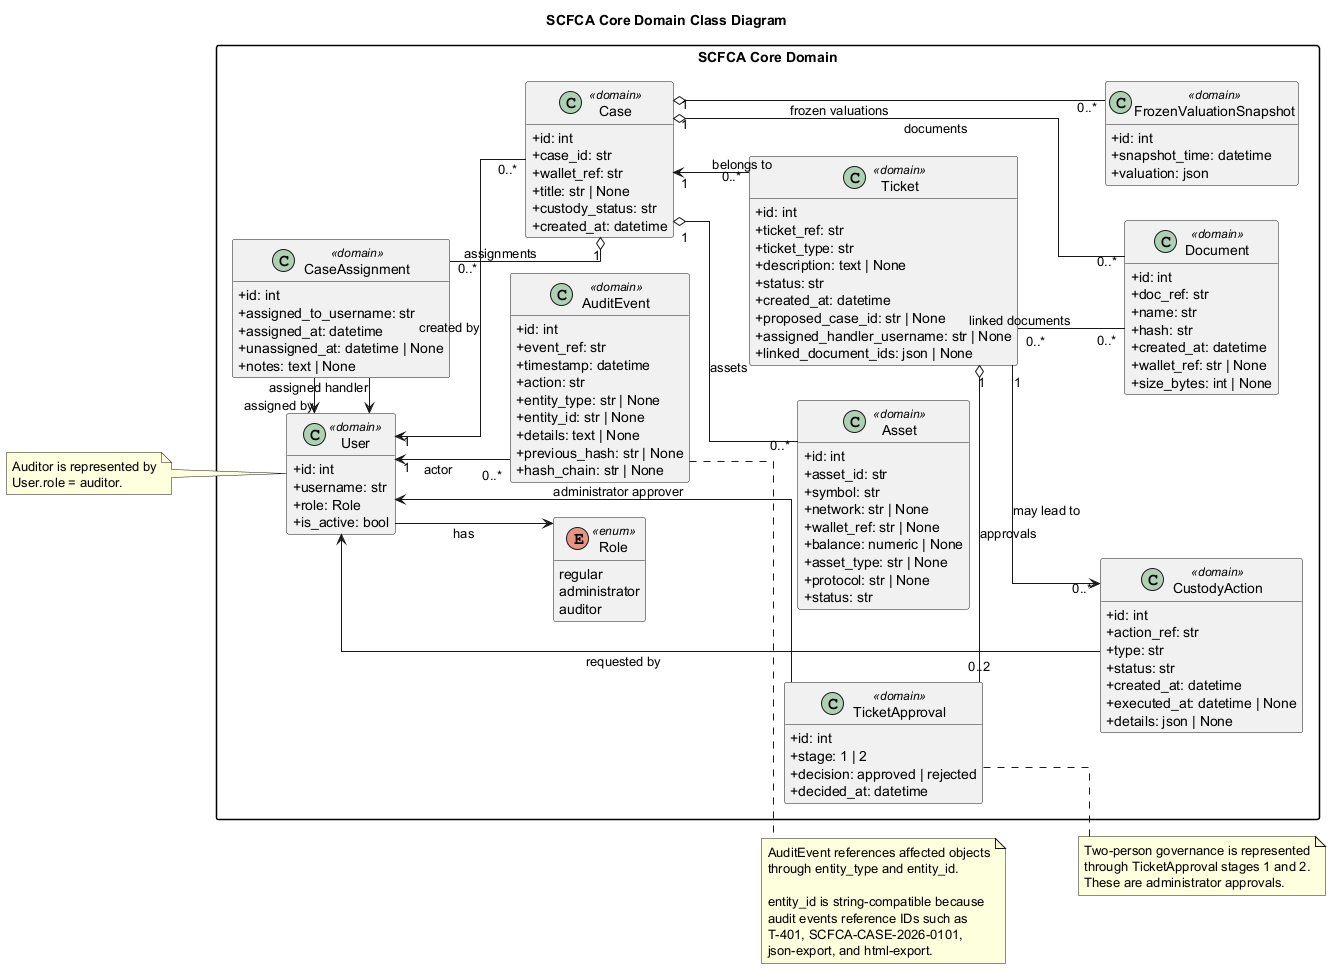
\includegraphics[width=0.95\textwidth]{figure25.png}
    \caption{Class diagram of the main backend domain models and relationships in the SCFCA project. PlantUML}
    \label{fig:class-diagram}
\end{figure}

\subsection{Log Integrity and Traceability Verification}

Audit evidence is validated by checking that custody actions generate traceable records protected by hash chaining, making unauthorized modification detectable. This supports the requirement that custody operations remain auditable, attributable, and reviewable over time. The logging and monitoring rationale is aligned with established guidance on computer security log management, where logs are treated as evidence for detection, accountability, and incident analysis~\cite{NIST80092}.

\subsection{Limitations of Validation}

The validation is limited to architectural correctness, proof-of-concept feasibility, and controlled security evidence within the academic scope of the thesis. Full production deployment, large-scale performance benchmarking, live blockchain transaction execution, real HSM integration, formal cryptographic verification, and independent external penetration testing remain outside the present validation scope.

\section{Toolchain and Development Environment}

The project uses Visual Paradigm for Secure Tropos and UML modeling, GitLab/GitHub for version control and traceability, Overleaf/LaTeX for the thesis document, and Visual Studio/Visual Studio Code for the proof-of-concept implementation. Detailed environment specifics are described in Chapter~6.


% =====================================================
\chapter{Threat Modeling}

\section{Threat Modeling Scope and Objectives}

This chapter presents the structured threat analysis performed for the Secure Custody Framework for Cryptocurrency Assets (SCFCA). The purpose of this chapter is not to provide a generic overview of cybersecurity threats, but to identify concrete risk scenarios that directly affect institutional cryptocurrency custody under criminal investigation contexts.

The threat model focuses on risks that may compromise:

\begin{itemize}
    \item Custody integrity (unauthorized asset manipulation or transfer)
    \item Role separation and governance constraints
    \item Auditability and non-repudiation
    \item Confidentiality of case-related information
    \item System availability during operational use
\end{itemize}

The analysis considers both external adversaries and malicious insiders. Given the institutional setting, insider threats are treated as equally critical as external attacks, particularly in scenarios involving privilege abuse or misuse of authorized access.

The output of this chapter is a structured set of misuse cases, associated attack paths, and mitigation measures that serve as the foundation for the formal security requirements and architectural controls defined in subsequent chapters.

\section{Threat Model Assumptions and Boundaries}

A clear definition of system boundaries and trust assumptions is necessary to ensure that the threat model remains realistic and technically coherent. The Secure Custody Framework for Cryptocurrency Assets (SCFCA) is modeled as an institutional custody management system operating within a controlled governmental environment.

\subsection{System Boundary}

The system boundary includes:

\begin{itemize}
    \item User authentication and role management mechanisms
    \item Case management and ticketing workflows
    \item Custody authorization logic (dual-control enforcement)
    \item Audit logging and traceability components
    \item Interfaces with the custody infrastructure responsible for cryptographic operations
\end{itemize}

The custody infrastructure (e.g., key management and transaction signing components) is treated as a controlled subsystem that executes approved operations but does not expose private keys directly to human actors.

External blockchain networks are considered outside the system boundary. The SCFCA interacts with them only through defined execution interfaces.

\subsection{Trust Assumptions}

The following trust assumptions are defined for this threat model:

\begin{itemize}
    \item Cryptographic primitives (e.g., hashing and digital signatures) are assumed to be secure and correctly implemented.
    \item The operating environment is institutionally controlled, but not immune to insider misuse.
    \item Administrators and case handlers may act maliciously if governance controls fail.
    \item External adversaries may attempt unauthorized access or system disruption.
    \item The underlying blockchain network behaves according to its consensus rules and is not considered compromised.
\end{itemize}

The threat model does not assume that all authenticated users are trustworthy. Instead, the architecture is explicitly designed to remain secure even if one privileged role attempts to abuse its access.

\subsection{Out-of-Scope Considerations}

The following aspects are considered outside the scope of this threat model:

\begin{itemize}
    \item Physical attacks against secure facilities
    \item Compromise of national infrastructure or state-level adversary control
    \item Formal cryptographic proof of algorithm correctness
    \item Economic attacks against blockchain consensus mechanisms
\end{itemize}

By clearly defining system boundaries and trust assumptions, the threat analysis in the following sections focuses on realistic governance failures, misuse scenarios, and technical abuse paths that directly impact institutional cryptocurrency custody.
\section{Threat Taxonomy}

Before defining specific misuse scenarios, it is useful to classify threats according to their origin and intent. In cybersecurity literature, threats are commonly categorized based on whether they originate internally or externally, and whether they result from malicious or non-malicious actions.

Figure~\ref{fig:threat_taxonomy} illustrates a general taxonomy of threats adapted from Jouini et al. (2014). The model distinguishes between external and internal threats and further classifies them into human, environmental, and technological sources. Human threats may be malicious (intentional attacks) or non-malicious (accidental actions), while environmental and technological threats are typically non-malicious and accidental in nature.

Within the context of the SCFCA, the primary focus of the threat model is on intentional human threats, both external adversaries and malicious insiders. However, accidental internal actions and technological failures are also considered where they may impact custody integrity, availability, or audit reliability.

Threat graphs are commonly used in cyber threat intelligence to model adversarial paths and objectives \cite{Lee2023}.

\begin{figure}
    \centering
    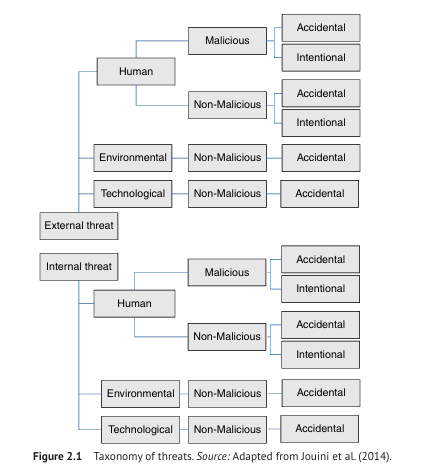
\includegraphics[width=1\linewidth]{figure 11.png}
    \caption{Taxonomy of threats. Adapted from Jouini et al. (2014), as discussed in cyber threat intelligence literature~\cite{Lee2023}.}
    \label{fig:threat_taxonomy}
\end{figure}


\section{Assets and Security Objectives}

Before identifying misuse scenarios, it is necessary to define the assets that require protection within the Secure Custody Framework for Cryptocurrency Assets (SCFCA). In this context, assets are not limited to cryptocurrency balances. They also include governance mechanisms and evidentiary records that are essential to institutional integrity.

\subsection{Primary Assets}

The primary assets considered in this threat model are:

\begin{itemize}
    \item \textbf{Seized cryptocurrency assets:} digital assets recorded under a CaseID and associated with frozen valuation snapshots.
    \item \textbf{Custody authorization workflows:} dual-control approval mechanisms governing sensitive operations such as transfers or reassignment.
    \item \textbf{Audit records and logs:} tamper-evident records of system actions, approvals, and execution outcomes.
    \item \textbf{Role and access control configurations:} definitions of privileges and enforcement of separation of duties.
    \item \textbf{Case-related information:} metadata, documentation, and sensitive information associated with investigations.
\end{itemize}

\subsection{Security Objectives}

Based on these assets, the following security objectives guide the threat analysis:

\begin{itemize}
    \item \textbf{Integrity:} Seized asset records and custody actions must not be modified without proper authorization and traceability.
    \item \textbf{Accountability:} All actions must be attributable to authenticated users and preserved in tamper-evident logs.
    \item \textbf{Separation of Duties:} No single actor must be able to initiate and execute custody-impacting actions independently.
    \item \textbf{Confidentiality:} Sensitive case information and identity mappings must be protected from unauthorized access.
    \item \textbf{Availability:} The system must remain operational for legitimate institutional use and resist disruption attempts.
\end{itemize}

These objectives define the protection goals that misuse cases attempt to violate. The following sections analyze concrete adversarial scenarios targeting these assets and objectives.

\section{Threat Graph–Based Misuse Analysis}

Threat graphs are used to visually represent the different paths an attacker may follow in order to achieve a specific objective. Instead of listing threats in isolation, a threat graph models how adversarial goals can be reached through multiple tactics and techniques.
This misuse-oriented analysis follows the principle that adversarial goals should be modeled explicitly so that security requirements can be derived from concrete abuse scenarios~\cite{Sindre2001,Choi2006}.

In this thesis, threat graphs are constructed for each high-risk misuse case identified in the SCFCA system. Each graph begins with a clearly defined malicious goal and works backwards through possible ATT\&CK tactics and techniques that an adversary could realistically apply within the institutional custody context.

This approach allows the analysis to focus on concrete attack paths rather than abstract threat categories. It also supports systematic mapping between adversarial techniques (MITRE ATT\&CK) and defensive countermeasures (MITRE D3FEND), ensuring that mitigation strategies address realistic attack sequences~\cite{MITREATTACK,MITRED3FEND}.

\subsection{MU-7 – Case Data Exfiltration (Threat Graph Analysis)}

\textbf{Attacker Goal.}  
Exfiltrate confidential case-related data or sensitive custody information from the SCFCA system.

Maintaining confidentiality of case narratives, personal data, and asset records is a critical institutional security objective. A successful exfiltration may compromise investigations, violate legal protections, and damage institutional credibility.

Working backwards from this malicious objective, the attacker must successfully apply the ATT\&CK tactic:

\begin{itemize}
    \item \textbf{Exfiltration – TA0010}
\end{itemize}

This may be achieved through one or more techniques, such as:

\begin{itemize}
    \item Exfiltration Over C2 Channel – T1041
    \item Exfiltration Over Alternative Protocol – T1048
    \item Exfiltration Over Web Service – T1567
     \item Exfiltration Over Physical Medium – TA1052
\end{itemize}

To perform exfiltration, the attacker must first obtain sufficient access privileges. This typically requires one or more of the following tactics:

\begin{itemize}
    \item Credential Access – TA0006
    \item Privilege Escalation – TA0004
    \item Lateral Movement – TA0008
    \item Execution – TA0002
\end{itemize}

In the SCFCA context, realistic attack paths include:

\begin{enumerate}
    \item Compromise of a Case Handler account via phishing (T1566) leading to Valid Account usage (T1078).
    \item Exploitation of broken access control allowing Insecure Direct Object Reference (IDOR).
    \item Insider abuse of legitimate access privileges.
\end{enumerate}

The corresponding defensive perspective maps to MITRE D3FEND mechanisms such as:

\begin{itemize}
    \item Multi-factor authentication enforcement
    \item Role-based access control validation
    \item Data access logging and anomaly detection
    \item Network monitoring for abnormal outbound data flows
\end{itemize}

By modeling the attack graph in this manner, the threat analysis highlights that preventing exfiltration requires not only perimeter controls, but also strict privilege enforcement, monitoring, and separation of duties within custody workflows.

\begin{figure}
    \centering
    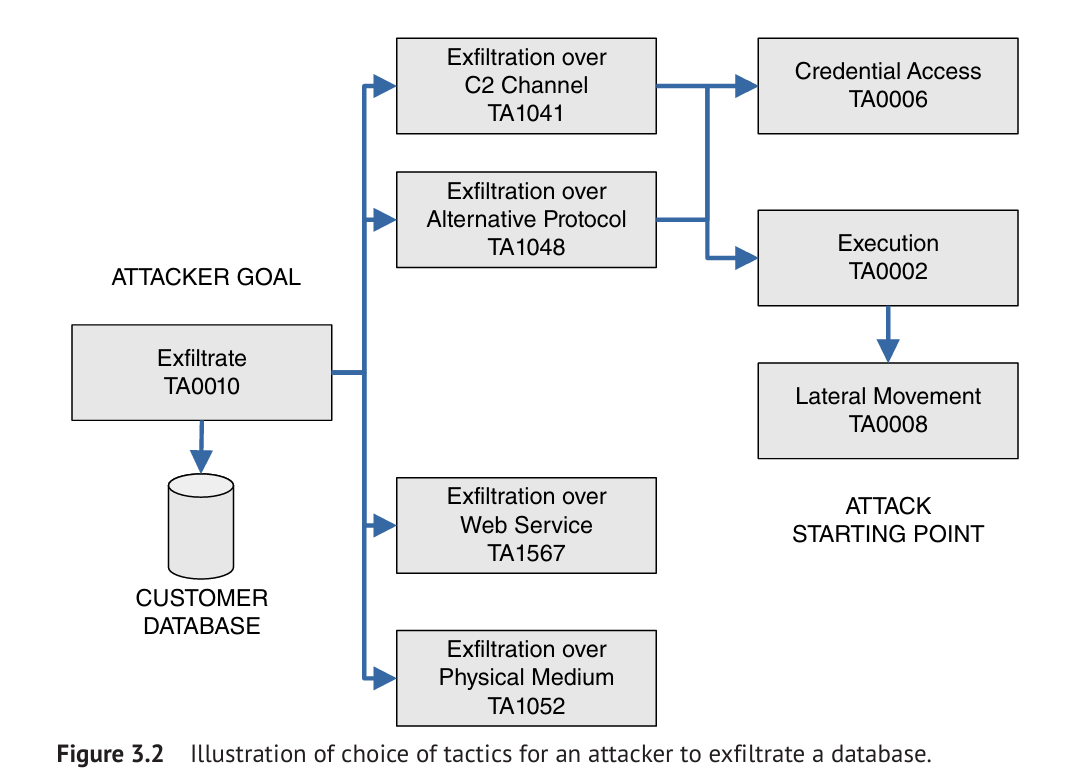
\includegraphics[width=0.75\linewidth]{figure10.png}
    \caption{Threat graph example for MU-7: Case Data Exfiltration~\cite{Lee2023}.}
    \label{fig:placeholder1}
\end{figure}

\subsection{MU-1 – Unauthorized Access (Threat Graph Analysis)}

\textbf{Attacker Goal.}  
The adversary aims to gain unauthorized access to the SCFCA system in order to later manipulate custody workflows, escalate privileges, or exfiltrate sensitive case information. Unauthorized access represents a foundational threat because it enables multiple secondary misuse scenarios.

Working backwards from this objective, the attacker must ultimately succeed in abusing a valid authentication context. Within the MITRE ATT\&CK framework, this corresponds primarily to:

\begin{itemize}
    \item \textbf{Valid Accounts – T1078}
\end{itemize}

Alternative direct approaches may also include:

\begin{itemize}
    \item \textbf{Brute Force – T1110}
\end{itemize}

To obtain valid credentials or authenticated session control, the attacker may follow several realistic attack paths in the institutional custody context.

These alternative paths form the basis of the MU-1 threat graph. Each branch illustrates a distinct route through which the attacker may reach the same malicious objective.

\textbf{Security Impact.}  
If successful, unauthorized access compromises the confidentiality of case data, undermines role-based access control enforcement, and may enable privilege escalation or manipulation of custody operations. In an institutional custody system, even temporary unauthorized access may jeopardize evidentiary integrity and institutional accountability.

\textbf{Defensive Considerations.}  
From a defensive perspective, mitigation requires layered controls including:

\begin{itemize}
    \item Multi-factor authentication enforcement
    \item Rate limiting and account lockout mechanisms
    \item Credential storage protection and endpoint monitoring
    \item Session binding and re-authentication for sensitive actions
    \item Continuous authentication logging and anomaly detection
\end{itemize}

The threat graph analysis demonstrates that preventing unauthorized access is not dependent on a single control, but on a combination of authentication hardening, credential protection, and session monitoring mechanisms.
\begin{figure}
    \centering
    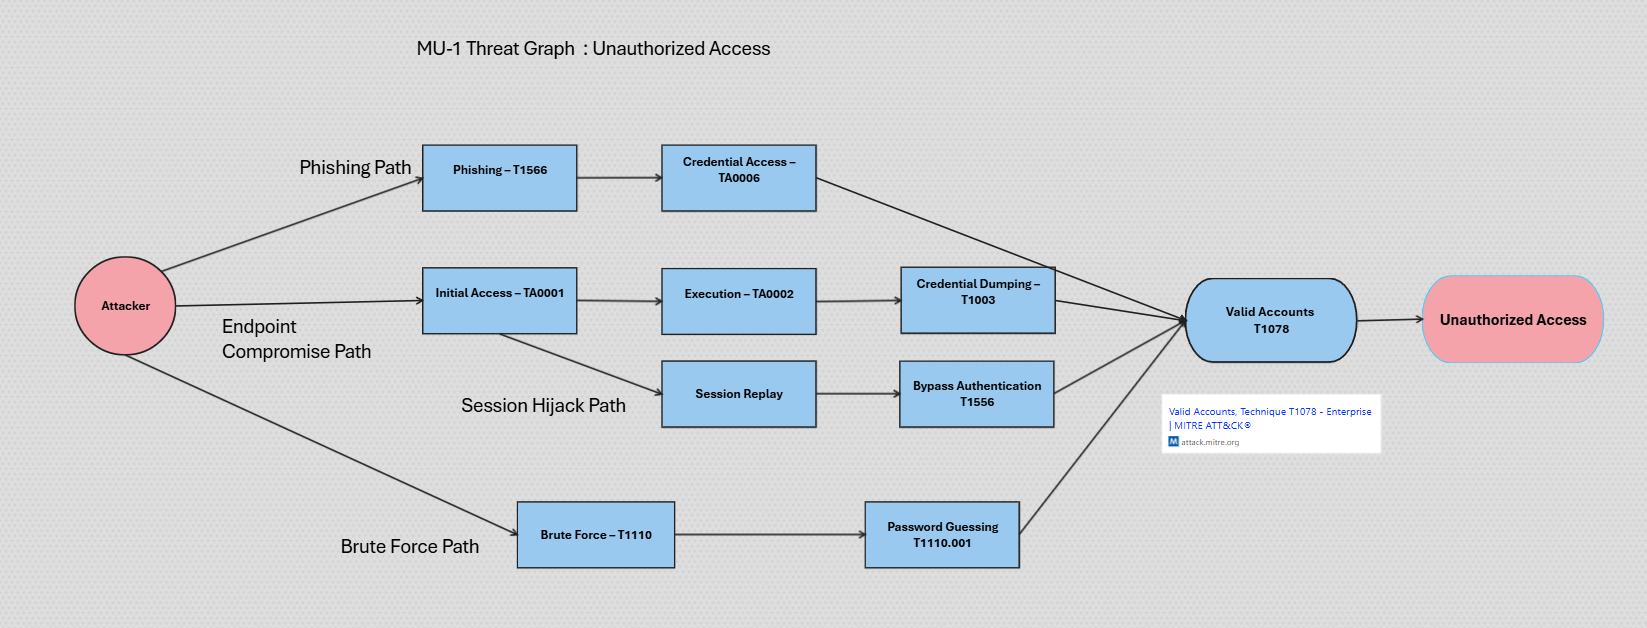
\includegraphics[width=1\linewidth]{figure9.png}
    \caption{MU-1 Threat Graph  : Unauthorized Access }
    \label{fig:placeholder3}
\end{figure}

\subsection{MU-2 – Privilege Escalation Exploit}

MU-2 addresses the scenario in which an attacker who already possesses some level of access to the SCFCA system attempts to escalate privileges in order to obtain administrative control. Unlike MU-1, which focuses on unauthorized initial access, this misuse case assumes that the adversary has successfully authenticated as a lower-privileged user (e.g., Case Handler) or has compromised a non-administrative account.

The attacker’s objective is to transition from limited access to elevated privileges, ultimately gaining Administrator-level capabilities within the custody system. This would enable manipulation of custody workflows, modification of asset records, or bypassing governance controls such as dual approval mechanisms.

From a MITRE ATT\&CK perspective, privilege escalation may involve the following tactics and techniques:

\begin{itemize}
    \item Exploitation for Privilege Escalation – T1068
    \item Abuse Elevation Control Mechanism – T1548
    \item Valid Accounts – T1078 (leveraging already compromised credentials)
    \item Exploitation of Application Vulnerabilities (e.g., injection, insecure API endpoints)
\end{itemize}

The threat graph for MU-2 models alternative attacker paths that converge on the attacker goal of achieving elevated privileges within SCFCA. Possible escalation routes include:

\begin{itemize}
    \item Exploiting misconfigured RBAC policies or improper role validation,
    \item Manipulating backend APIs to bypass authorization checks,
    \item Exploiting software vulnerabilities to gain code execution in a privileged context,
    \item Abusing token handling or session management flaws to assume a higher-privileged identity.
\end{itemize}

All attack branches ultimately converge on the attacker goal:

\begin{center}
\textit{Administrator-Level Access to SCFCA}
\end{center}

\begin{figure}
    \centering
    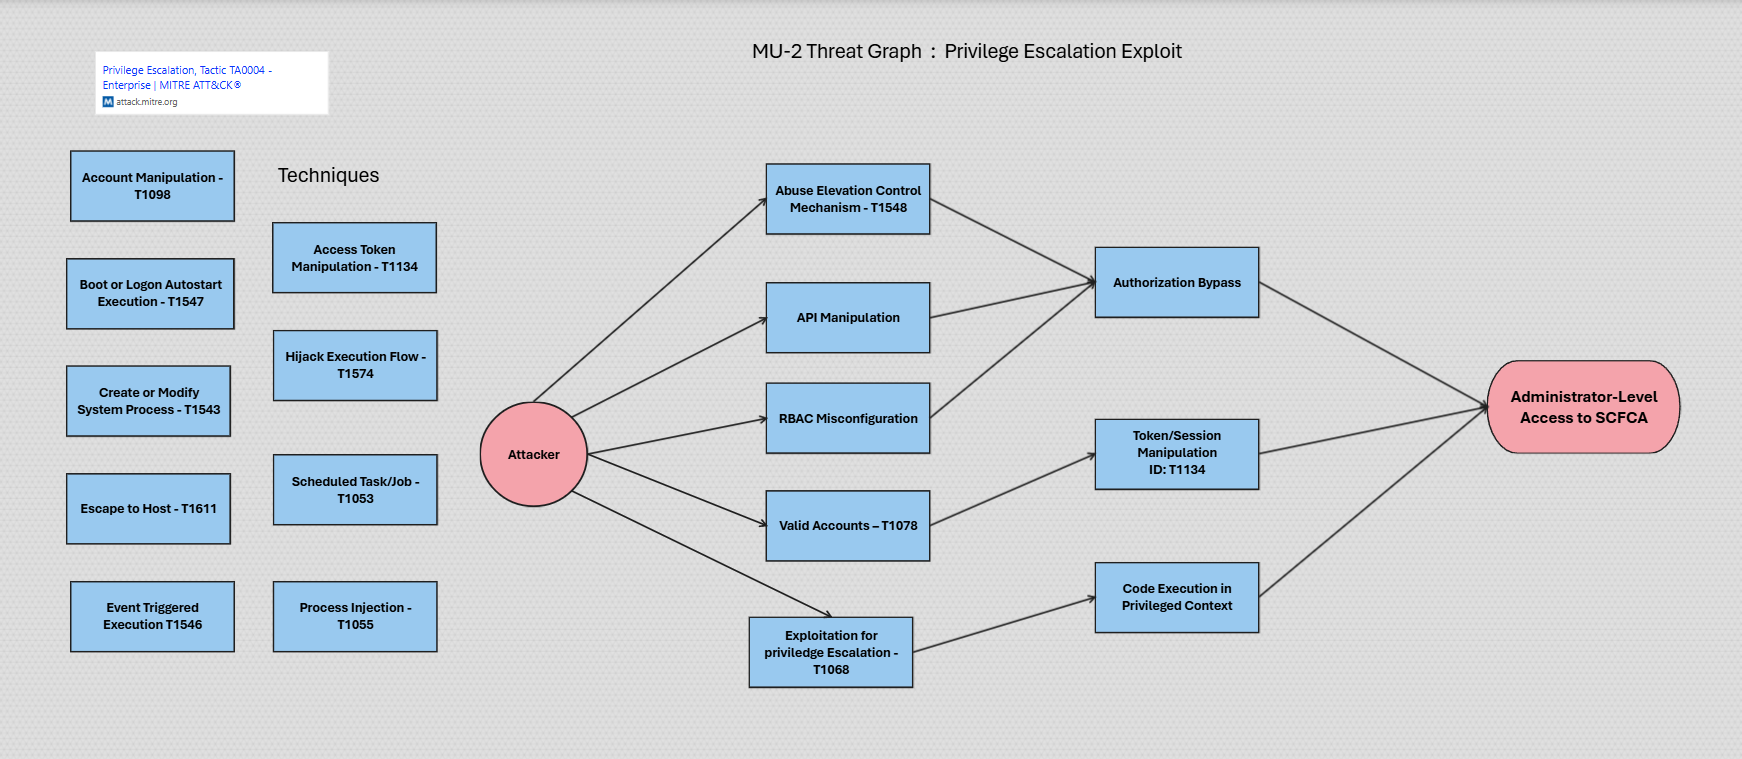
\includegraphics[width=1\linewidth]{figure 12.png}
    \caption{MU-2 – Privilege Escalation Threat Graph}
    \label{fig:placeholder4}
\end{figure}

From a defensive standpoint, the architecture mitigates these escalation paths through strict role-based access control (SR-1), controlled role assignment mechanisms (SR-4), privilege escalation prevention controls (SR-3), and enforcement of authorization checks at every security-sensitive endpoint. Additionally, audit logging and traceability mechanisms reduce the likelihood that unauthorized privilege transitions remain undetected.

By modeling privilege escalation explicitly as a graph of converging attacker options, the analysis highlights that elevated access is rarely the result of a single failure. Rather, it typically emerges from combinations of misconfigurations, insufficient authorization enforcement, or exploitable vulnerabilities. The architectural design of SCFCA therefore enforces privilege boundaries structurally, rather than relying solely on procedural controls.

The threat graphs developed in this chapter are grounded in structured threat intelligence sources, most notably the MITRE ATT\&CK and MITRE D3FEND frameworks, which provide detailed mappings of adversarial tactics, techniques, and corresponding defensive countermeasures. These sources, complemented by broader open intelligence and the technical knowledge acquired throughout this Master's program—particularly in secure software design and security engineering best practices—form the analytical foundation of the SCFCA threat model. 

By systematically mapping misuse scenarios to established attack techniques and defensive controls, this analysis moves beyond abstract risk discussion and establishes a concrete, evidence-based understanding of how the system may be targeted and how those threats can be mitigated. 

With this structured threat knowledge in place, the work can now transition from adversarial analysis to architectural design. The next chapter builds directly upon these findings to define the security-driven architecture of the SCFCA framework, ensuring that its components, controls, and governance mechanisms are explicitly aligned with the identified threat landscape.



% =====================================================
\chapter{System Architecture}
\section{System Actors}
The Secure Custody Framework for Cryptocurrency Assets (SCFCA) operates within an institutional environment involving multiple actors with clearly separated responsibilities and access privileges. The explicit definition of system actors is essential to enforce separation of duties, prevent abuse of privileges, and ensure accountability and auditability across all custody operations.

All interactions with the system are performed by authenticated users operating under predefined roles. Each role is associated with a specific set of permissions that strictly limit the actions the actor can perform.

\begin{figure}
    \centering
    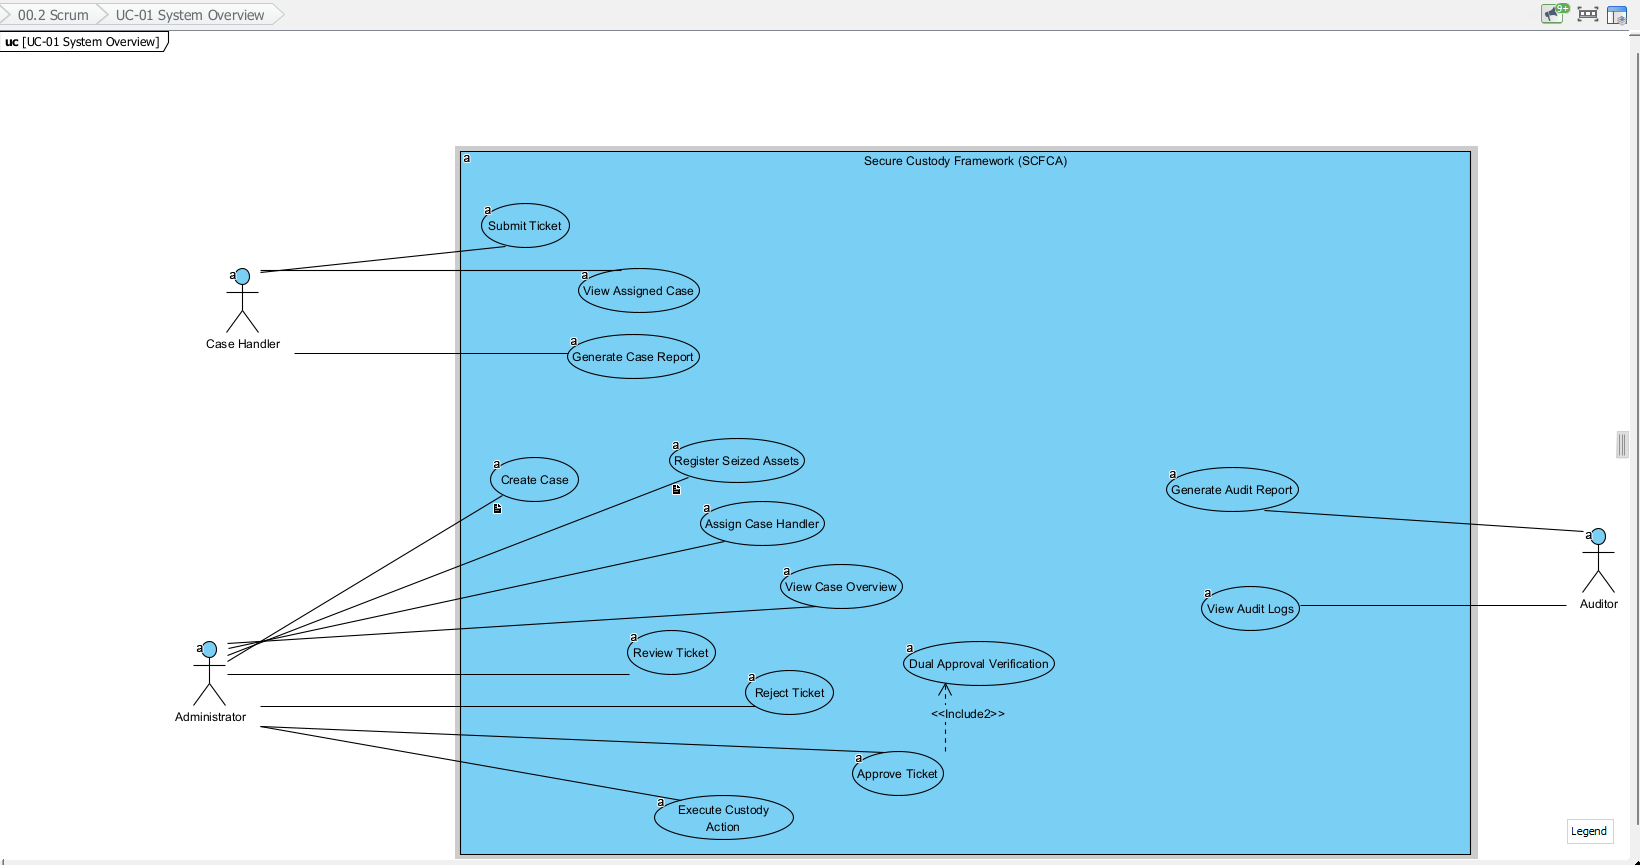
\includegraphics[width=1\linewidth]{Figure 1 . System overview ( simplified first idea ).png}
    \caption{ System overview ( simplified first idea , use cases)}
    \label{fig:system-overview}
\end{figure}

\subsection{Identity Representation}
All users within the system are represented internally by pseudonymous UserIDs. These identifiers do not encode the user’s role, real-world identity, or organizational position. Role information and access privileges are managed separately through the system’s access control mechanisms. This design minimizes information leakage, prevents bias, and ensures that audit records remain operationally meaningful without exposing unnecessary personal data.

The mapping between UserIDs and real-world identities is restricted to authorized administrative processes outside the scope of the audit role.


\subsection{Case Handler}
The Case Handler represents the authorized investigative authority responsible for managing a specific case (e.g., a prosecutor or designated investigative officer). This actor is responsible for initiating all custody-related requests within the system.

\begin{figure}
    \centering
    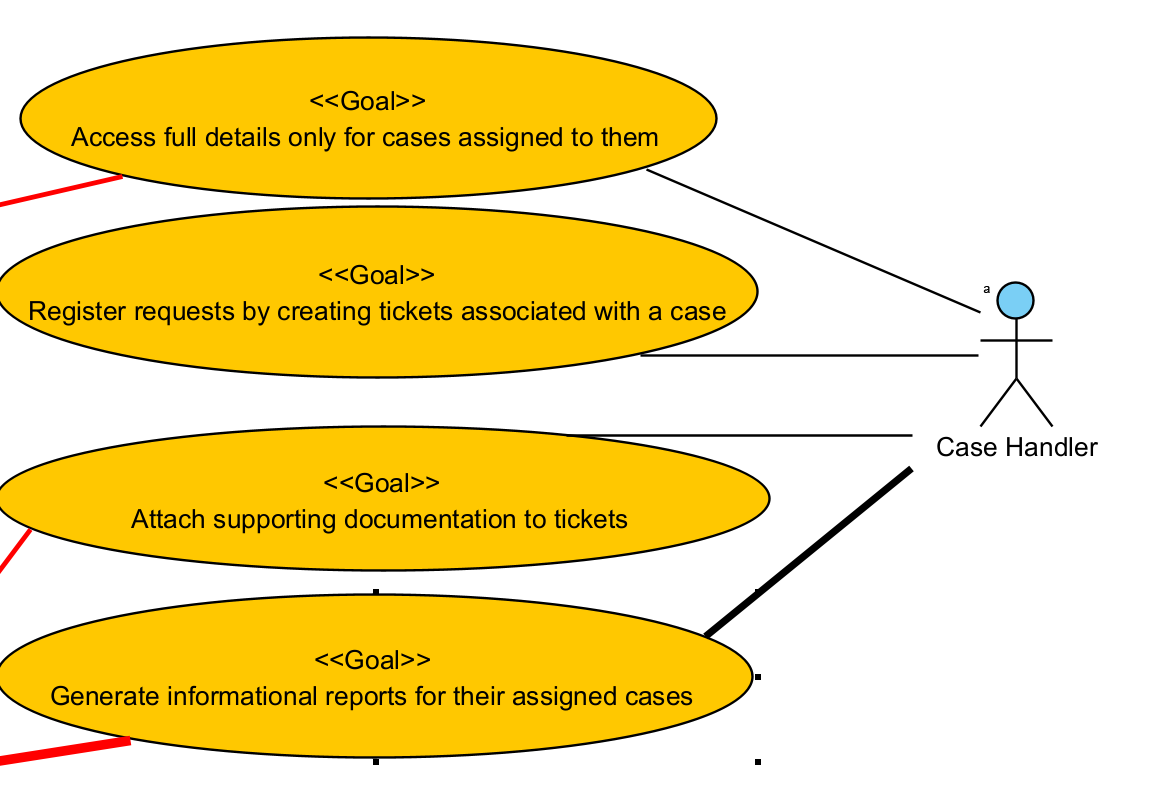
\includegraphics[width=1\linewidth]{Figure2.png}
    \caption{Tropo Analysis diagram (case handler’s goals)}
    \label{fig:placeholder2}
\end{figure}

The Case Handler can:

\begin{itemize}
\item Access full details only for cases assigned to them
\item Register requests by creating tickets associated with a case
\item Attach supporting documentation to tickets
\item Generate informational reports for their assigned cases
\end{itemize}

The Case Handler cannot:
\begin{itemize}
\item Modify case or asset data directly
\item Execute asset transfers or conversions
\item Approve or reject tickets
\item Access detailed information of cases not assigned to them 
\end{itemize}


\subsection{Administrator}

The Administrator is responsible for managing institutional configuration, creating cases,
assigning case handlers, and reviewing governance requests submitted through tickets.
Administrators act as control actors within the custody workflow, but they cannot initiate custody-related tickets themselves.

\begin{figure}
    \centering
    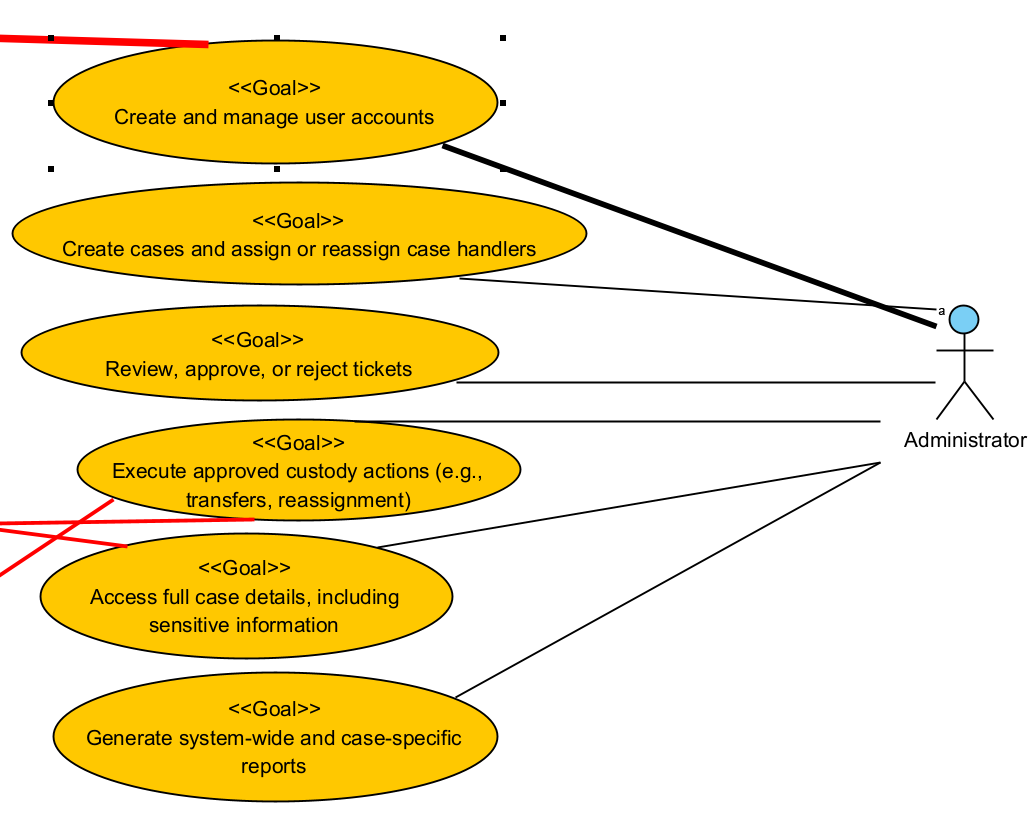
\includegraphics[width=1\linewidth]{Figure3.png}
    \caption{Tropo Analysis Diagram ( Administrator’s goals)}
    \label{fig:placeholder}
\end{figure}


The Administrator can:

\begin{itemize}
    \item Create and manage user accounts.
    \item Create cases and assign them to Case Handlers.
    \item Review, approve, or reject tickets submitted by Case Handlers.
    \item Participate in the dual-approval workflow for custody-impacting actions.
    \item Generate system-wide and case-specific reports according to authorization rules.
\end{itemize}


The Administrator cannot:

\begin{itemize}
    \item Initiate tickets.
    \item Execute custody-impacting actions without the required approval workflow.
    \item Modify original seized asset facts or frozen valuation snapshots.
    \item Delete CaseIDs, tickets, documents, or audit records.
    \item Bypass the dual-approval workflow.
\end{itemize}

All administrative actions are recorded in the audit log and remain subject to later review.

\subsection{Auditor}
The Auditor is responsible for independent oversight of the system’s operation. This role is strictly read-only and is designed to detect irregularities, verify compliance, and support accountability.
The Auditor can:
\begin{itemize}
\item View all CaseIDs
\item Monitor all system actions and events
\item Review tickets, approvals, rejections, and execution outcomes
\item Generate and download audit reports for any time period or case
\item Verify integrity of logs and documentation
\end{itemize}


The Auditor cannot:
\begin{itemize}
\item Modify cases, assets, tickets, or assignments
\item Approve or reject tickets
\item Execute custody actions
\item Access real-world identities of users
\item Access personally identifiable information (PII) or confidential case narratives.
\end{itemize}
\begin{figure}
    \centering
    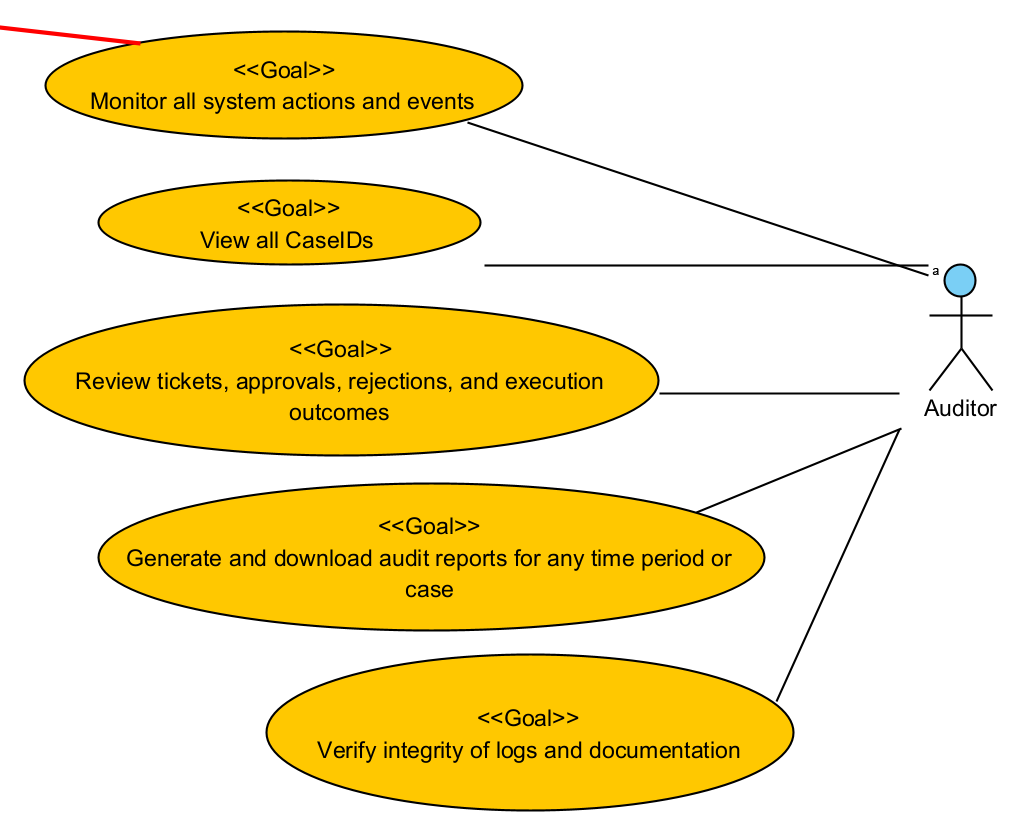
\includegraphics[width=1\linewidth]{Figure4.png}
    \caption{Tropo Analysis Diagram ( Auditor’s goals) }
    \label{fig:Auditor,Secure Tropos}
\end{figure}

\subsection{External Adversary}
The External Adversary represents any unauthorized entity attempting to compromise the system. This includes attackers seeking to gain unauthorized access, escalate privileges, manipulate custody operations, or tamper with audit records. While not interacting through legitimate system interfaces, this actor is considered in the system’s threat model to ensure resilience against external attacks. Misuse cases: 

MU-1 Unauthorized Access

MU-2 Privilege Escalation Exploit

MU-9 DoS

MU-7 (if credentials stolen)

\begin{figure}
    \centering
    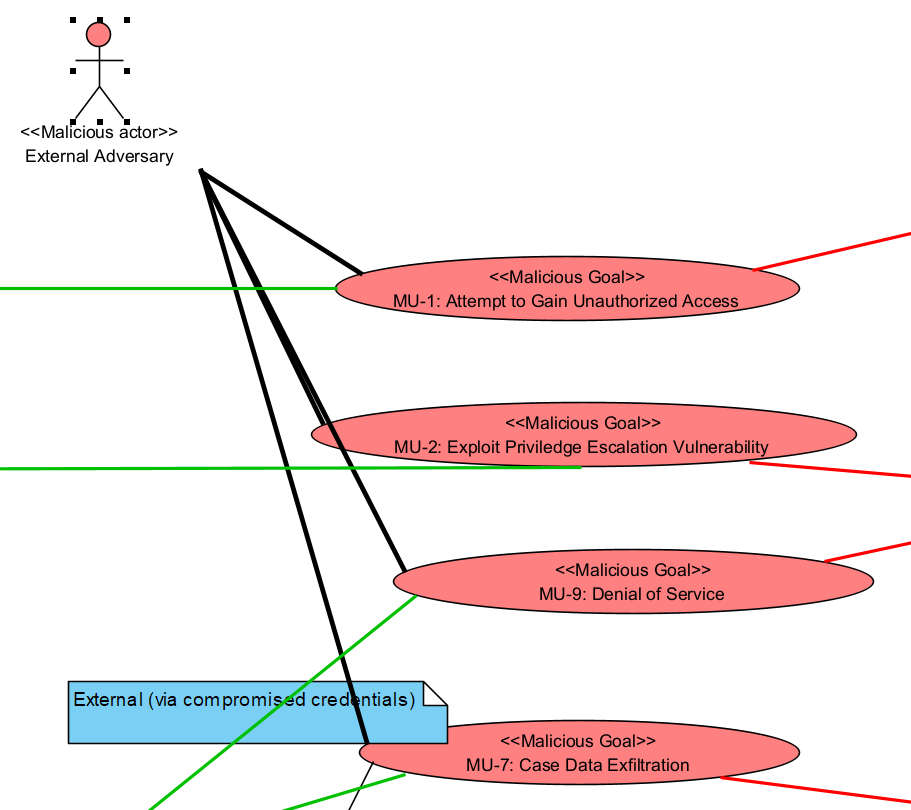
\includegraphics[width=1\linewidth]{Figure5.png}
    \caption{Tropo Analysis Diagram ( External Adversary’s goals)}
    \label{fig:placeholder}
\end{figure}



\subsection{Malicious Insider}
The Malicious Insider represents an authenticated internal user who intentionally abuses legitimate access privileges to compromise custody integrity, confidentiality, or auditability.
This actor may correspond to:

- A compromised Case Handler

- A compromised Administrator

- A privileged technical operator

- Any authorized user acting with malicious intent


Unlike the External Adversary, the Malicious Insider already possesses valid authentication credentials and operates within legitimate system boundaries. The risk arises not from bypassing authentication mechanisms, but from abusing authorized privileges, exploiting workflow weaknesses, or attempting to manipulate governance controls.

The Malicious Insider may attempt to:

\begin{itemize}
\item Bypass dual approval mechanisms
\item Manipulate ticket states
\item Modify or tamper with audit logs
\item Alter seized asset records
\item Replace or manipulate supporting documentation
\item Replay or duplicate custody executions
\item Access sensitive case data beyond authorized scope
\end{itemize}

The design of SCFCA explicitly mitigates insider threats through:
\begin{itemize}
\item Strict separation of duties
\item Dual administrative approval enforcement
\item Immutable asset records
\item Tamper-evident audit logging
\item Least-privilege role enforcement
\item Full action traceability and non-repudiation
\end{itemize}

The inclusion of the Malicious Insider actor ensures that the framework addresses not only perimeter security risks but also internal abuse scenarios, which are particularly critical in institutional custody environments.

Misuse cases : 

MU-3 Bypass Dual Approval

MU-4 Log Tampering

MU-5 Asset Manipulation

MU-6 Document Tampering

MU-8 Replay Execution

MU-7 (internal abuse)

\begin{figure}
    \centering
    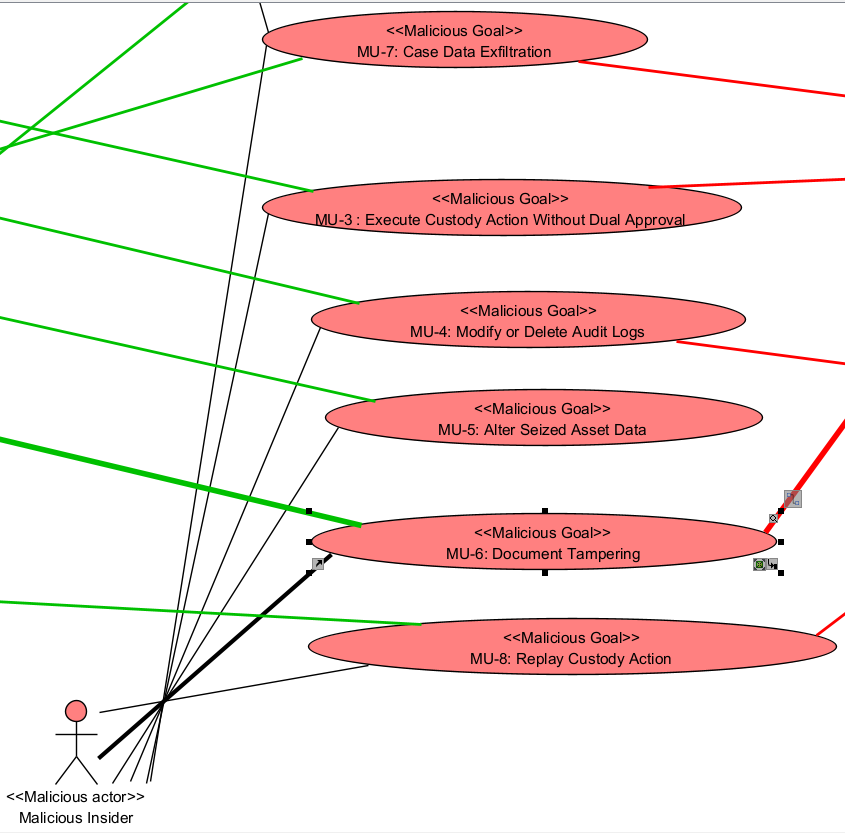
\includegraphics[width=1\linewidth]{Figure6.png}
    \caption{Tropo Analysis Diagram ( Malicious Insider’s goals)}
    \label{fig:placeholder}
\end{figure}



\subsection{Misuse Case – Threat and Mitigation Mapping}

In addition to legitimate use cases, the Secure Custody Framework for Cryptocurrency Assets (SCFCA) explicitly models malicious goals through misuse cases. These misuse cases represent intentional attempts by adversarial actors to compromise the confidentiality, integrity, availability, or auditability of institutional cryptocurrency custody operations.

Unlike functional use cases, which describe intended system behavior, misuse cases describe adversarial objectives and potential exploitation paths. Their inclusion serves two primary purposes:

1.To formally identify security-relevant threats against the system.

2.To ensure that every identified threat is mitigated by specific security controls and requirements.


Each misuse case defines:

a. A malicious goal (what the adversary aims to achieve),

b. Potential attack vectors (how the goal may be attempted),

c. Corresponding mitigation measures (which system requirements or controls prevent, detect, or contain the threat).



This structured mapping establishes traceability between:


Misuse Case → Security Control → Functional/Security Requirement


By linking each malicious goal to explicit mitigation mechanisms, the framework ensures that security controls are not arbitrary but directly justified by threat analysis.


Furthermore, this approach supports:
\begin{itemize}
\item Defense-in-depth design,
\item Verification of security coverage,
\item Architectural traceability between Chapter 3 (Requirements) and Chapter 5 (Design and Architecture).
\end{itemize}


The following table summarizes the identified misuse cases, their attack vectors, and the corresponding mitigation measures embedded in the system requirements.



\begin{longtable}{|p{1.2cm}|p{3.2cm}|p{3.2cm}|p{3.8cm}|p{4.5cm}|}
\caption{Misuse Case - Threat \& Mitigation Mapping}
\\\hline
\textbf{ID} & \textbf{Misuse Case} & \textbf{Malicious Goal} & \textbf{Typical Attack Vectors} & \textbf{Mitigation Measures (Mapped to Requirements)} \\
\\\hline
\endfirsthead

\hline
\textbf{ID} & \textbf{Misuse Case} & \textbf{Malicious Goal} & \textbf{Typical Attack Vectors} & \textbf{Mitigation Measures (Mapped to Requirements)} \\
\hline
\endhead

MU-1 & Attempt to Gain Unauthorized Access & Log into the system without valid credentials & Brute force, credential stuffing, phishing, stolen credentials & SR-5 MFA; SR-6 Re-authentication for sensitive actions; SR-7 Session traceability; SR-8 Logging \\
\hline

MU-2 & Exploit Privilege Escalation Vulnerability & Become Administrator from Case Handler or external account & RBAC misconfiguration, API manipulation, injection attacks & SR-1 Least Privilege; SR-3 Privilege Escalation Prevention; SR-4 Controlled Role Assignment \\
\hline

MU-3 & Execute Custody Action Without Dual Approval & Trigger asset transfer without two admin approvals & Ticket state manipulation, direct API call to execution endpoint, race condition exploit & SR-12 Dual Approval Enforcement; FR-17 Ticket Approval Rule; SR-13 Execution Traceability \\
\hline

MU-4 & Modify or Delete Audit Logs & Hide malicious activity & Database manipulation, filesystem access, log deletion & SR-9 Tamper-Evident Logs; SR-10 Log Deletion Prevention; SR-11 Non-Repudiation; Append-only storage \\
\hline

MU-5 & Alter Seized Asset Data & Modify asset quantities or frozen valuation snapshot & DB injection, insider manipulation, unauthorized admin change & SR-15 Asset Data Immutability; FR-12 Asset Facts Immutability \\
\hline

MU-6 & Document Tampering & Replace or alter supporting PDF evidence & File replacement, DB hash modification & SR-16 Document Integrity Verification; FR-23 Document Hashing \\
\hline

MU-7 & Case Data Exfiltration & Access PII or confidential case narratives & IDOR, broken access control, API abuse & FR-3 RBAC; SR-18 Restricted Access; SR-19 Audit Privacy Boundary \\
\hline

MU-8 & Replay Custody Action & Execute same transfer twice & Resubmitting transaction, manipulating execution state & FR-27 Transaction Linking; SR-13 Execution Traceability \\
\hline

MU-9 & Denial of Service & Prevent system usage & API flooding, login flooding, ticket spam & NFR-1 Availability; Rate limiting \\
\hline

\end{longtable}


% =====================================================


MU-1 (Unauthorized Access) → threatens → "Access full details for assigned cases"


MU-2 (Privilege Escalation) → threatens → "Create and manage user accounts"


MU-3 (Bypass Dual Approval) → threatens → "Execute approved custody actions"


MU-4 (Modify Logs) → threatens → "Monitor all system actions and events"


MU-5 (Alter Asset Data) → threatens → "Maintain seized asset records"


MU-6 (Document Tampering) → threatens → "Attach supporting documentation"

MU-7 (Data Exfiltration) → threatens → "Access full case details"

MU-8 (Replay Action) → threatens → "Execute approved custody actions"

MU-9 (DoS) → threatens → "System availability / Generate reports / Submit tickets"

\begin{figure}
    \centering
    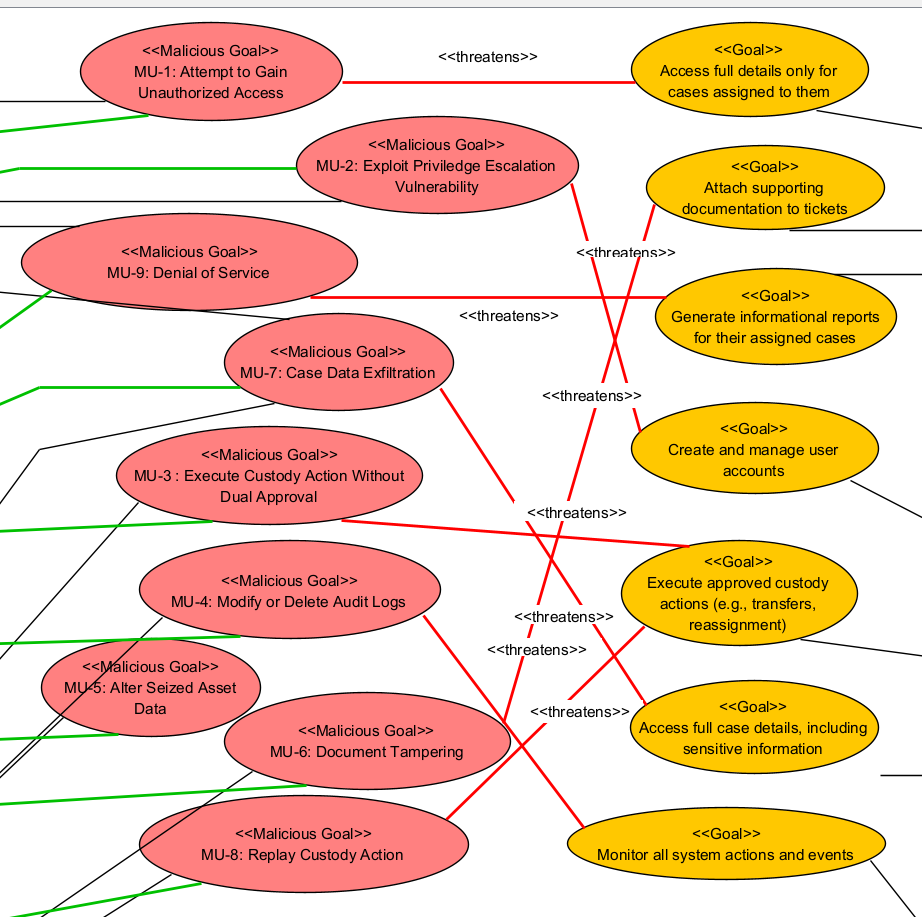
\includegraphics[width=1\linewidth]{Figure7.png}
    \caption{Tropo Analysis Diagram (Threat-goals relations)}
    \label{fig:placeholder}
\end{figure}

\subsection{Mitigation Measures (Security Countermeasures)}

In order to address identified misuse cases and threat scenarios, a set of security mitigation measures is defined at the design level. These measures represent security goals and architectural constraints that directly counteract the malicious objectives modeled in the threat analysis.
Each mitigation measure is derived from the formal Security Requirements defined in Section 3.3 and is conceptually mapped to one or more misuse cases. The purpose of this mapping is to demonstrate traceability between identified threats and the corresponding technical or procedural controls implemented within the Secure Custody Framework for Cryptocurrency Assets (SCFCA).

\begin{figure}
    \centering
    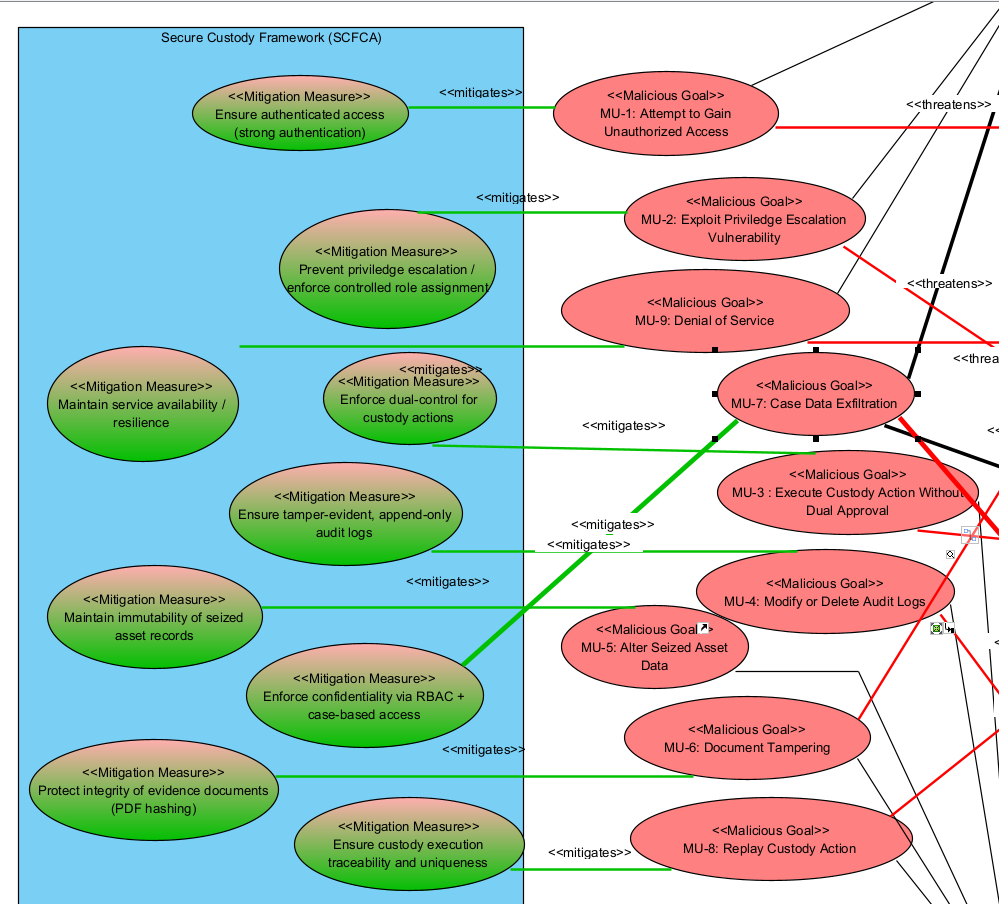
\includegraphics[width=1\linewidth]{Figure8.png}
    \caption{Tropo Analysis Diagram (Mitigation Measures )}
    \label{fig:placeholder}
\end{figure}

The mitigation measures focus on:

Preventing unauthorized access and privilege escalation

Enforcing dual control and separation of duties

Protecting custody integrity and asset immutability

Ensuring auditability and non-repudiation

Preserving confidentiality of sensitive case information

Maintaining system availability and resilience

\begin{longtable}{|p{1.2cm}|p{4.2cm}|p{4.8cm}|p{3.5cm}|}

\caption{Mitigation Measures Use Cases -- Threat \& Mitigation Mapping}
\label{tab:mitigation-mapping} \\

\hline
\textbf{ID} & \textbf{Mitigation Measure } & \textbf{Requirements} & \textbf{Misuse Case} \\
\hline
\endfirsthead

\hline
\textbf{ID} & \textbf{Mitigation Measure } & \textbf{Requirements} & \textbf{Misuse Case} \\
\hline
\endhead

MM-1 & Ensure authenticated access (strong authentication) & SR-5 MFA; SR-6 Re-authentication for sensitive actions; SR-7 Session traceability; SR-8 Logging & Attempt to Gain Unauthorized Access \\
\hline

MM-2 & Prevent privilege escalation / enforce controlled role assignment & SR-1 Least Privilege; SR-3 Privilege Escalation Prevention; SR-4 Controlled Role Assignment & Exploit Privilege Escalation Vulnerability \\
\hline

MM-3 & Enforce dual-control for custody actions & SR-12 Dual Approval Enforcement; FR-17 Ticket Approval Rule; SR-13 Execution Traceability & Execute Custody Action Without Dual Approval \\
\hline

MM-4 & Ensure tamper-evident, append-only audit logs & SR-9 Tamper-Evident Logs; SR-10 Log Deletion Prevention; SR-11 Non-Repudiation; Append-only storage & Modify or Delete Audit Logs \\
\hline

MM-5 & Maintain immutability of seized asset records & SR-15 Asset Data Immutability; FR-12 Asset Facts Immutability & Alter Seized Asset Data \\
\hline

MM-6 & Protect integrity of evidence documents (PDF hashing) & SR-16 Document Integrity Verification; FR-23 Document Hashing & Document Tampering \\
\hline

MM-7 & Enforce confidentiality via RBAC + case-based access & FR-3 RBAC; SR-18 Restricted Access; SR-19 Audit Privacy Boundary & Case Data Exfiltration \\
\hline

MM-8 & Ensure custody execution traceability and uniqueness & FR-27 Transaction Linking; SR-13 Execution Traceability & Replay Custody Action \\
\hline

MM-9 & Maintain service availability / resilience & NFR-1 Availability; Rate limiting & Denial of Service \\
\hline

\end{longtable}

This structured threat–mitigation relationship ensures that security controls are not added reactively, but are embedded as explicit design constraints within the system architecture.

\section{Custody Infrastructure and Software Trust Boundaries}

The following two components are not human actors but architectural subsystems whose security properties directly affect the governance model defined above.

\subsection{Custody Infrastructure}

The Custody Infrastructure represents the technical subsystem responsible for performing cryptographic custody operations and interacting with external blockchain networks. It encompasses components for secure key management, transaction construction, transaction signing, and transaction broadcasting.
The Custody Infrastructure operates as a trusted technical boundary within the overall system architecture. It enforces cryptographic controls independently from user-facing application logic and ensures that custody-related operations are executed only upon validated and approved instructions originating from the governance layer of the system.
The Custody Infrastructure:

\begin{itemize}
\item Operates autonomously based on approved and validated instructions
\item Does not represent a human actor
\item Does not expose private keys or sensitive cryptographic material to any user
\item Executes custody actions only after dual administrative approval has been verified
\item Logs all cryptographic and execution-related operations for audit and traceability purposes
\end{itemize}
The Custody Infrastructure is treated as a high-trust component within the architecture. However, its operations remain fully traceable through system-level logging and audit mechanisms to preserve accountability and evidentiary integrity.

\subsection{Secure Software Architecture, Trust Boundaries, and Dependency Governance}

Beyond institutional actors and governance workflows, the SCFCA must also be understood as a modern layered software system. Its security therefore depends not only on the permissions of human users, but also on the interactions between application components, third-party dependencies, runtime environments, containerized services, and supporting infrastructure.

At the software level, the architecture can be interpreted as consisting of several layers: a client-facing interface layer, an application layer implementing custody and governance logic, a persistence layer for structured records, an audit layer responsible for security-relevant event recording, and a supporting infrastructure layer including the operating environment, container runtime, and deployment pipeline. These layers do not operate under identical trust assumptions. In particular, third-party libraries, framework packages, and container base images must be treated as components with limited trust rather than as implicitly secure building blocks.

This perspective leads to an important architectural principle for SCFCA: security-critical decisions must remain concentrated in controlled backend components and must never depend on the trustworthiness of the presentation layer or of client-controlled input. For this reason, authorization, dual approval enforcement, execution traceability, document integrity verification, and audit generation are treated as server-side responsibilities. The frontend may request actions, but it does not determine whether those actions are allowed.

A second consequence concerns dependency governance. Because the SCFCA relies on external software components, dependency selection and maintenance become part of the security architecture. The system should therefore follow a policy of minimizing unnecessary dependencies, preferring mature and actively maintained libraries, documenting component provenance, and reviewing dependency impact when updates are introduced. This does not eliminate software supply chain risk, but it reduces exposure and improves traceability.

Finally, this trust-boundary view aligns the architecture with a Zero Trust interpretation of software composition: no external component is considered trustworthy merely because it is popular or widely used. Trust must instead be supported by evidence such as maintenance history, version control, vulnerability status, integrity verification, and controlled integration into the overall design. In the SCFCA context, this is particularly important because failures in supporting software may indirectly undermine custody integrity, confidentiality, or auditability even when the higher-level governance model remains conceptually sound.

\section{Functional Requirements}
\subsection{Identity, Accounts, Roles}
\begin{figure}
    \centering
    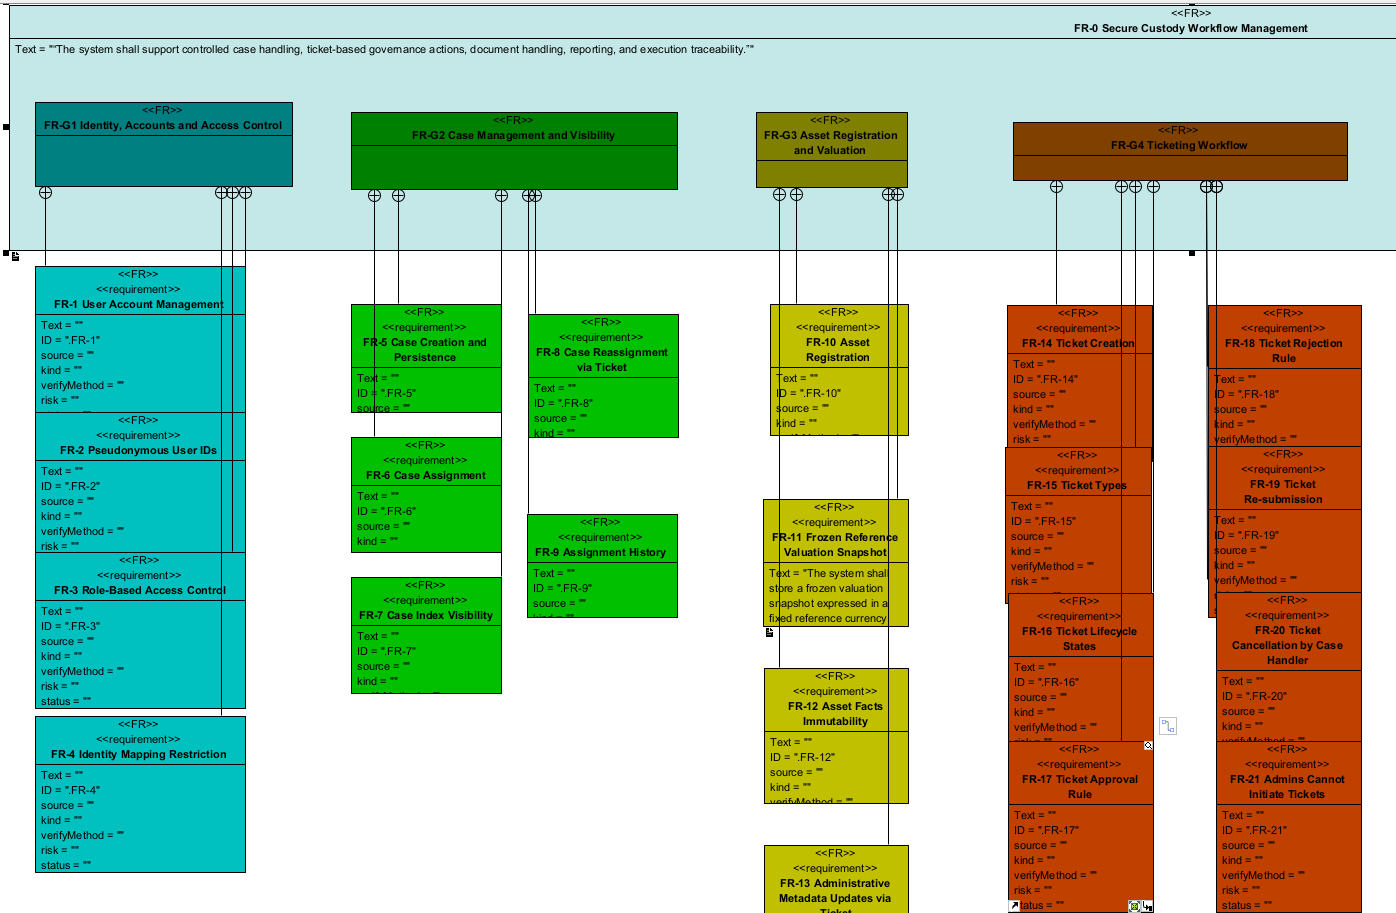
\includegraphics[width=1\linewidth]{figure13.png}
    \caption{Functional requirements model for identity, case management, asset registration, and ticketing workflow.}
    \label{fig:placeholder}
\end{figure}
\subsubsection{FR-1 User Account Management}

The system shall allow administrators to create and manage user profiles for the following roles: Case Handler, Administrator, Auditor (and optionally System Manager if needed for maintenance).

\subsection{Identity, Accounts, and Access Control}

\subsubsection{FR-2 Pseudonymous User IDs}


The system shall assign each user a pseudonymous UserID used in the UI and logs, where the UserID does not encode role or real identity.

\subsubsection{FR-3 Role-Based Access Control (RBAC)}


The system shall enforce RBAC so that users can perform only actions authorized by their role and by case assignment rules.

\subsubsection{FR-4 Identity Mapping Restriction}


The system shall restrict real-identity data (names/PII of case subjects and user real identities) so that Audit cannot view it. Administrators and assigned case handlers may access case-subject PII only for their authorized cases.

\subsection{Case Management and Visibility}


\subsubsection{FR-5 Case Creation and Persistence}

The system shall allow administrators to create cases identified by a unique, random, non-semantic CaseID. CaseIDs shall never be deleted.

\subsubsection{FR-6 Case Assignment}

Each case shall be assigned to exactly one case handler at a time. The system shall prevent access to detailed case data by non-assigned case handlers.

\subsubsection{FR-7 Case Index Visibility}

All authenticated users shall be able to view the list of CaseIDs, while access to case details is restricted according to role and assignment.

\subsubsection{FR-8 Case Reassignment via Ticket}

The system shall allow case reassignment only through an approved reassignment ticket.


\subsubsection{FR-9 Assignment History}

The system shall maintain an immutable history of all case assignments and reassignments, including timestamps, involved UserIDs, ticket reference, and admin approvals.

\subsection{Asset Registration and Valuation}


\subsubsection{FR-10 Asset Registration}

The system shall allow the registration of seized assets under a CaseID, including asset type (e.g., BTC, SOL), quantity, and relevant metadata.

\subsubsection{FR-11 Frozen Reference Valuation Snapshot}

The system shall store a frozen valuation snapshot expressed in a fixed reference currency (e.g., USDT) calculated at the moment of seizure/registration (with timestamp and valuation source). This snapshot shall be immutable.

\subsubsection{FR-12 Asset Facts Immutability}

The system shall prevent modification of the original seized asset facts (asset types and quantities) and the frozen reference valuation snapshot once recorded.

\subsubsection{FR-13 Administrative Metadata Updates via Ticket}

The system shall allow administrative updates/corrections only for permitted metadata fields (e.g., notes, documentation links, status fields), and only via approved tickets. No case handler can directly change stored case/asset records.

\subsection{Ticketing Workflow (the core)}

\subsubsection{FR-14 Ticket Creation}

The system shall allow a case handler to create a ticket linked to a CaseID, containing: request type, description, and supporting documentation.

\subsubsection{FR-15 Ticket Types}

The system shall support typed tickets at minimum:
\begin{itemize}
\item Transfer request (custody action)
\item Conversion request (custody action) (may be “out of system” in PoC)
\item Case reassignment request (governance action)
\item Metadata correction/update request (administrative action)
\end{itemize}

\subsubsection{FR-16 Ticket Lifecycle States}

Each ticket shall have a lifecycle state: Open, In Process, Closed.

\subsubsection{FR-17 Ticket Approval Rule (Two Admins)}

A ticket shall be executed only if both administrators approve it (parallel approval; order does not matter).

\subsubsection{FR-18 Ticket Rejection Rule}

If any administrator rejects a ticket, the ticket shall be Closed as Rejected, no system changes shall occur, and both administrators shall add notes explaining the rejection.

\subsubsection{FR-19 Ticket Re-submission}

After rejection, the case handler may open a new ticket addressing the rejection requirements; rejected tickets remain permanently recorded.

\subsubsection{FR-20 Ticket Cancellation by Case Handler}

The case handler shall be able to cancel a ticket only if it has not yet received both approvals and no execution/system changes have begun.

\subsubsection{FR-21 Admins Cannot Initiate Tickets}

Administrators shall not be able to create tickets. If an admin requires an action, the admin must request the case handler to open a ticket.


\subsection{Document Handling (PDF + integrity)}

\subsubsection{FR-22 PDF-Only Documentation}

All supporting documents attached to tickets shall be uploaded and stored as PDF files only.

\subsubsection{FR-23 Document Integrity Hashing}

Upon upload, the system shall compute and store a cryptographic hash (e.g., SHA-256) for each PDF and associate it with the CaseID/TicketID, uploader UserID, and timestamp.


\subsection{Reporting}

\subsubsection{FR-24 Audit Reporting (System-Wide)}

The Auditor shall be able to generate and download full activity reports for any period, any case, and any user, excluding protected PII and confidential case narrative details.

\subsubsection{FR-25 Case Reporting (Per Case)}

Administrators and the assigned case handler shall be able to generate and download per-case reports (PDF) reflecting the current case state for evidentiary or court usage.

\subsubsection{FR-26 Reports are Informational}

Generated reports shall be informational snapshots and shall not modify system state or constitute authorization for actions.

\begin{figure}
    \centering
    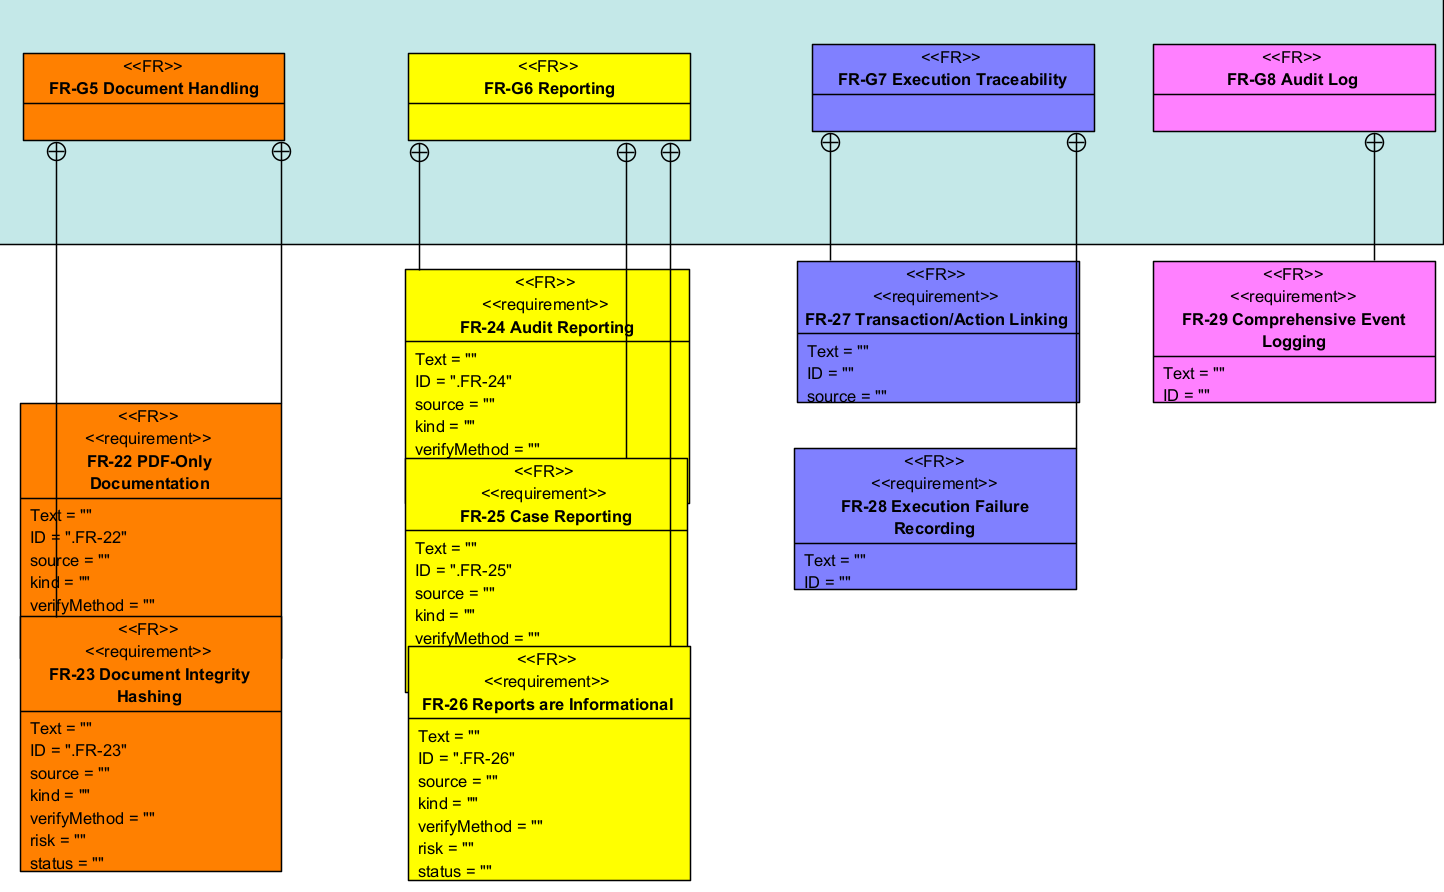
\includegraphics[width=1\linewidth]{figure14..png}
    \caption{Functional requirements model for document handling, reporting, execution traceability, and audit logging.}
    \label{fig:placeholder}
\end{figure}

\subsection{Execution Traceability}

\subsubsection{FR-27 Transaction/Action Linking}

For custody actions (e.g., transfer), the system shall link the executed action to the originating ticket and record identifiers and status (e.g., transaction hash, timestamp).

\subsubsection{FR-28 Execution Failure Recording}

If an approved action cannot be executed (technical failure), the system shall record the failure reason, preserve traceability, and close the ticket with a final outcome indicating failure (no silent retries without logging).

\subsection{Audit Log (syslog-level)}

\subsubsection{FR-29 Comprehensive Event Logging}

The system shall record every meaningful action and security-relevant event (authentication events, ticket lifecycle changes, approvals/rejections, policy changes, report downloads, document uploads, assignment changes, execution attempts) in an audit log with actor UserID and timestamp.


\section{Security Requirements}

Although security requirements are often classified as non-functional requirements in traditional software engineering, in this work they are defined as a separate category due to their central role in addressing insider threats, custody integrity, and auditability within institutional cryptocurrency custody systems.

The following security requirements specify the controls necessary to ensure confidentiality, integrity, accountability, and traceability throughout the custody lifecycle. These requirements are derived from the threat landscape identified in Chapter 2 and are designed to mitigate risks related to privilege abuse, unauthorized asset manipulation, and tampering with audit evidence.

Figures~\ref{fig:security-requirements-part-1} and~\ref{fig:security-requirements-part-2}
present the security requirements model developed in Visual Paradigm. The model is divided
into two parts for readability. The first part groups the requirements related to access
control, privilege management, authentication, session security, audit integrity, non-repudiation,
and custody dual control. The second part groups the requirements related to asset
immutability, document integrity, case identifier persistence, confidentiality, privacy boundaries,
and pseudonymous identity representation.

\subsection{Access Control and Privilege Management}

\subsubsection{SR-1 Least Privilege Enforcement}

The system shall enforce a least-privilege access control model ensuring that each role can perform only explicitly authorized actions.

\begin{figure}
    \centering
    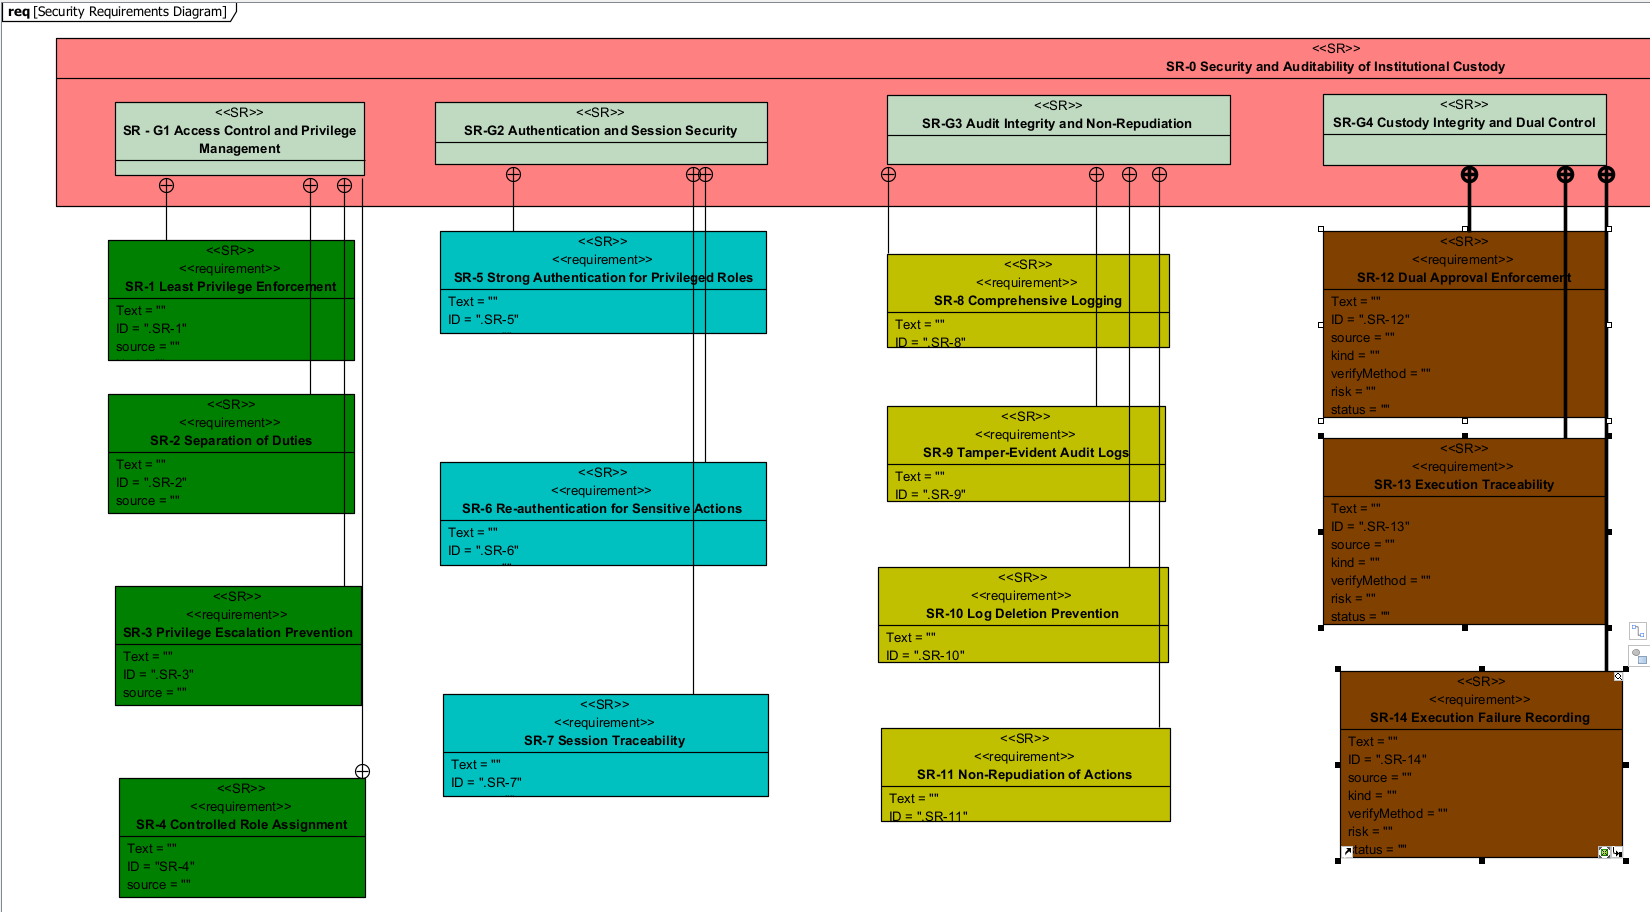
\includegraphics[width=1\linewidth]{figure15.png}
    \caption{Security requirements model for access control, authentication, audit integrity, and custody dual control.}
    \label{fig:security-requirements-part-1}
\end{figure}
\subsubsection{SR-2 Separation of Duties}

The system shall enforce strict separation of duties such that no single actor can both initiate and approve custody-impacting operations.

\subsubsection{SR-3 Privilege Escalation Prevention}

The system shall prevent unauthorized role modifications and privilege escalation attempts.

\subsubsection{SR-4 Controlled Role Assignment}

Role creation and modification shall be restricted to Administrators and shall be fully logged.

\subsection{Authentication and Session Security}

\subsubsection{SR-5 Strong Authentication for Privileged Roles}

Administrators shall use multi-factor authentication (MFA) when performing privileged operations.

\subsubsection{SR-6 Re-authentication for Sensitive Actions}

The system shall require explicit re-authentication before executing custody-impacting actions.

\subsubsection{SR-7 Session Traceability}

Authentication events and session activities shall be recorded and associated with the corresponding UserID.


\subsection{Audit Integrity and Non-Repudiation}

\subsubsection{SR-8 Comprehensive Logging}

The system shall record all security-relevant events, including authentication events, ticket lifecycle transitions, approvals, rejections, assignment changes, document uploads, report generation, and custody execution attempts.

\subsubsection{SR-9 Tamper-Evident Audit Logs}

Audit logs shall be implemented as append-only records and protected using integrity mechanisms (e.g., cryptographic hash chaining) to ensure that unauthorized modifications are detectable.

\subsubsection{SR-10 Log Deletion Prevention}

No actor shall be able to delete or alter existing audit records.

\subsubsection{SR-11 Non-Repudiation of Actions}

All actions shall be attributable to a specific authenticated UserID.

\subsection{Custody Integrity and Dual Control}

\subsubsection{SR-12 Dual Approval Enforcement}

Custody-impacting operations shall require independent approval from two Administrators. A single rejection shall prevent execution.

\subsubsection{SR-13 Execution Traceability}

Every executed custody operation shall be linked to its originating ticket and recorded with execution status and relevant identifiers.

\subsubsection{SR-14 Execution Failure Recording}

If an approved custody operation fails during execution, the system shall record the failure outcome and preserve full traceability.

\subsection{Data Integrity and Evidence Protection}

\begin{figure}
    \centering
    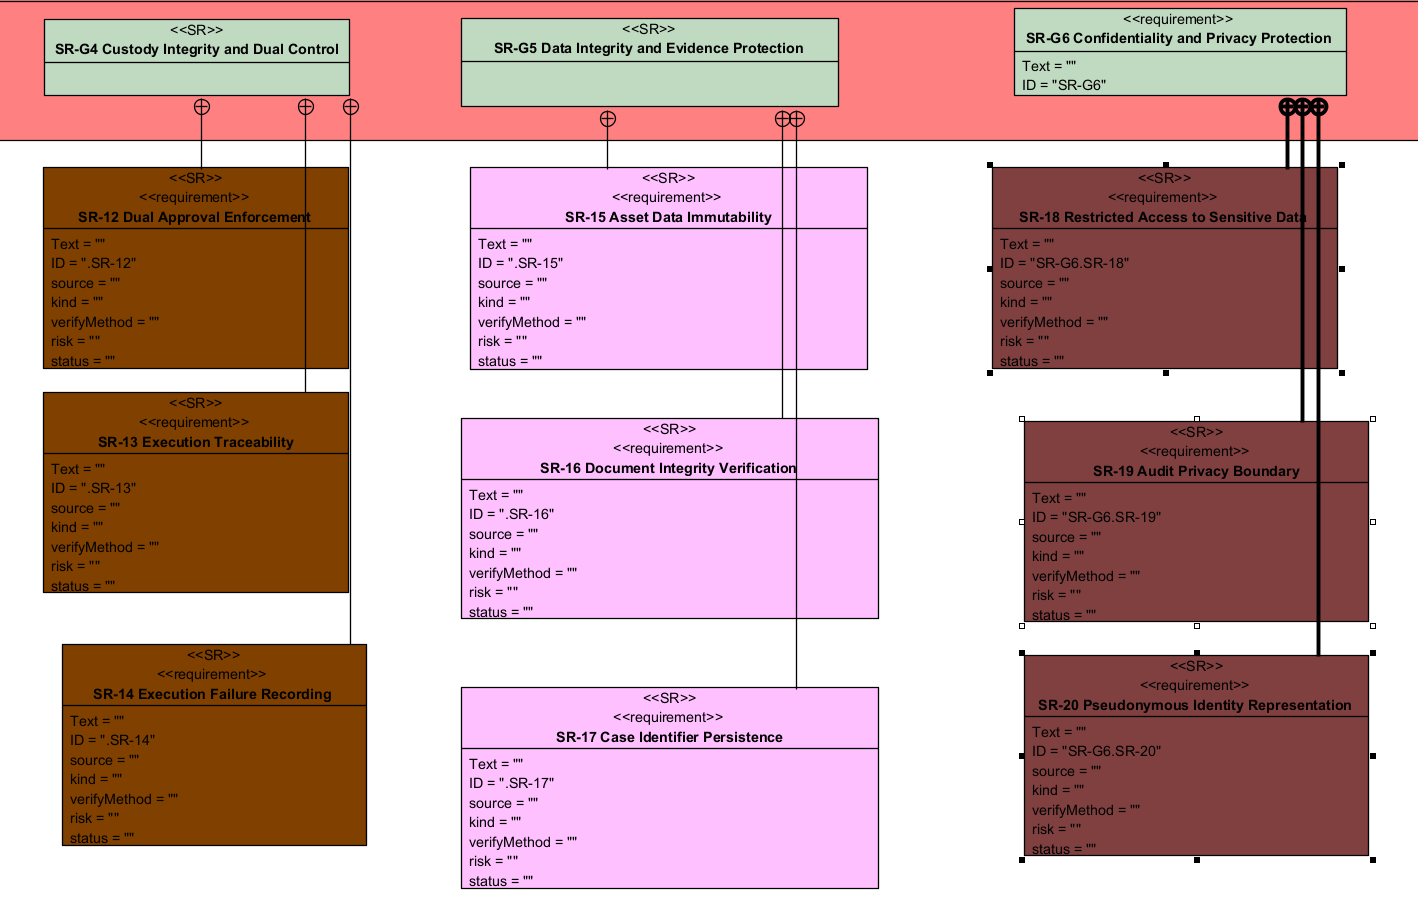
\includegraphics[width=1\linewidth]{figure16.png}
    \caption{Security requirements model for custody integrity, data protection, confidentiality, and privacy controls.}
    \label{fig:security-requirements-part-2}
\end{figure}

\subsubsection{SR-15 Asset Data Immutability}

Original seized asset records and frozen valuation snapshots shall be immutable.

\subsubsection{SR-16 Document Integrity Verification}

All uploaded PDF documents shall be integrity-protected using cryptographic hashing. Any integrity mismatch shall be logged as a security incident.

\subsubsection{SR-17 Case Identifier Persistence}

CaseIDs shall be immutable and shall never be deleted.

\subsection{Confidentiality and Privacy Protection}

\subsubsection{SR-18 Restricted Access to Sensitive Data}

Sensitive case data and PII shall only be accessible to authorized Administrators and the assigned Case Handler.

\subsubsection{SR-19 Audit Privacy Boundary}

The Auditor shall be restricted from accessing PII and confidential case content while retaining full visibility into operational and security events.

\subsubsection{SR-20 Pseudonymous Identity Representation}

System interfaces and audit records shall use pseudonymous UserIDs that do not encode role or real-world identity.

\section{Non-Functional Requirements}

The following non-functional requirements define the operational qualities and system-level constraints of the Secure Custody Framework for Cryptocurrency Assets (SCFCA). These requirements ensure that the system remains reliable, maintainable, and usable within an institutional environment while preserving evidentiary integrity.

Figure~\ref{fig:non-functional-requirements-model} presents the non-functional requirements model developed in Visual Paradigm. These requirements define the operational qualities expected from the SCFCA framework, including availability, reliability, long-term data retention, backup and recovery, response time, scalability assumptions, role-based interface clarity, workflow transparency, reporting capability, log retention integrity, modularity, and configurability of the reference currency.

\begin{figure}
    \centering
    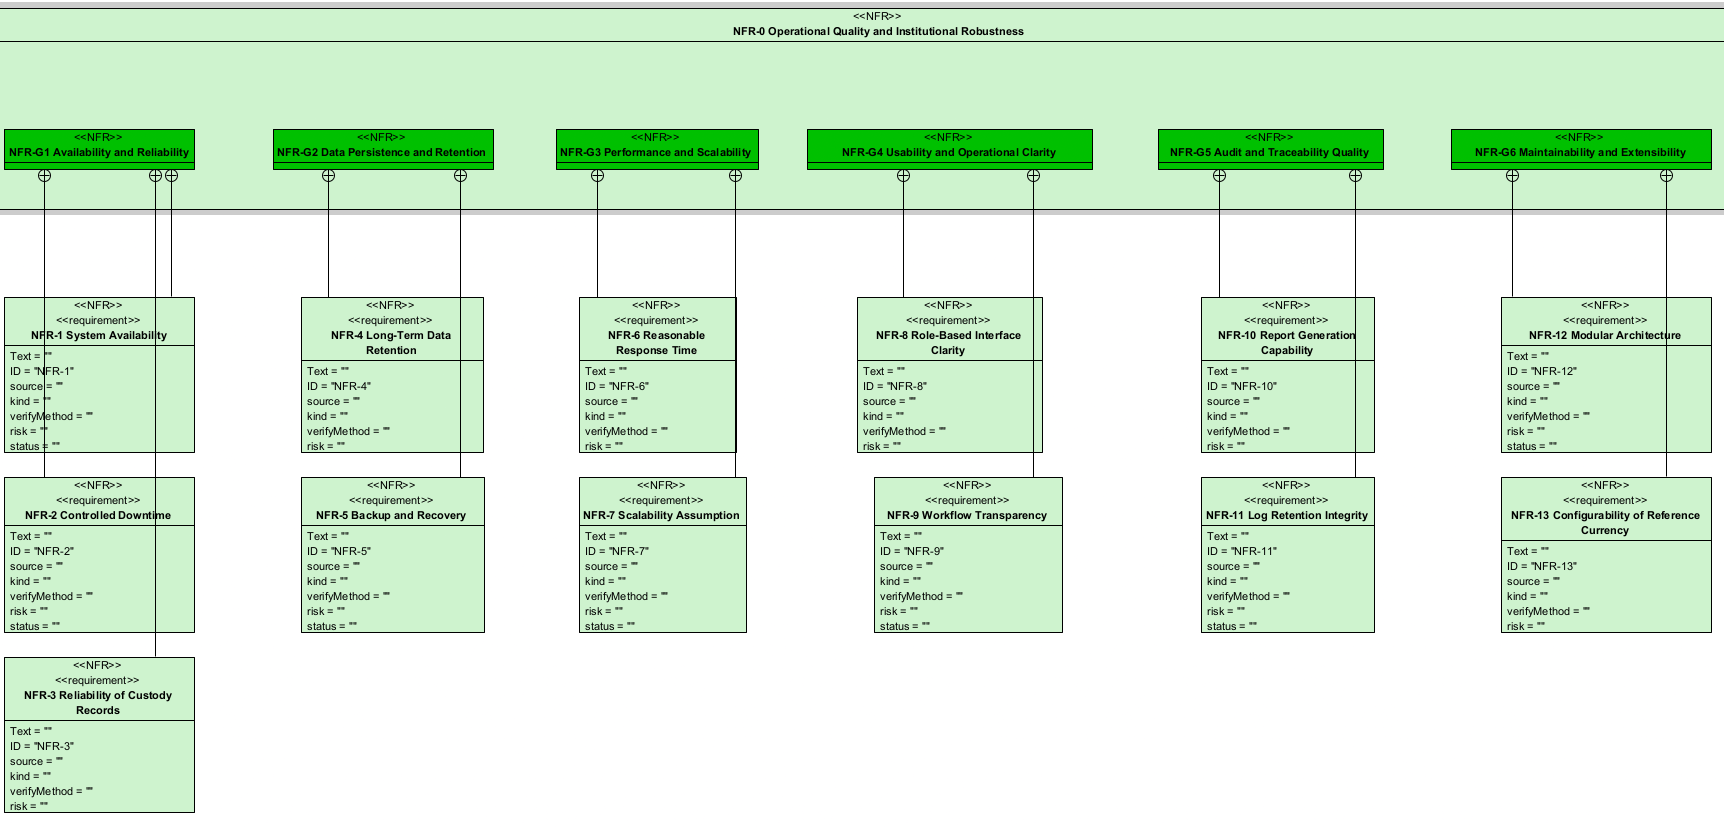
\includegraphics[width=1\linewidth]{figure18.png}
    \caption{Non-functional requirements model for operational quality, reliability, traceability, and maintainability.}
    \label{fig:non-functional-requirements-model}
\end{figure}

\subsection{Availability and Reliability}

\subsubsection{NFR-1 System Availability}

The system shall be designed to provide high availability during institutional working hours, minimizing operational downtime.

\subsubsection{NFR-2 Controlled Downtime}

Maintenance operations shall be performed in a controlled manner and shall not compromise data integrity or audit records.

\subsubsection{NFR-3 Reliability of Custody Records}

The system shall ensure that case and asset records remain consistent and recoverable in the event of system interruption.

\subsection{Data Persistence and Retention}

\subsubsection{NFR-4 Long-Term Data Retention}

All case records, tickets, audit logs, and documentation shall be retained for the entire legal lifecycle of the case and shall not be automatically deleted.

\subsubsection{NFR-5 Backup and Recovery}

The system shall support secure backup and recovery mechanisms to prevent permanent loss of institutional data.

\subsection{ Performance and Scalability}

\subsubsection{NFR-6 Reasonable Response Time}

The system shall provide reasonable response times for standard operations such as case viewing, ticket creation, and report generation.

\subsubsection{NFR-7 Scalability Assumption}

The architecture shall be designed to support the management of multiple concurrent cases without degradation of core functionality.

(Note: As a proof-of-concept implementation, extreme-scale performance optimization is outside scope.)

\subsection{Usability and Operational Clarity}

\subsubsection{NFR-8 Role-Based Interface Clarity}

The user interface shall clearly reflect role-based permissions to minimize operational errors.

\subsubsection{NFR-9 Workflow Transparency}

Ticket status transitions and approval states shall be clearly visible to authorized users.


\subsection{Audit and Traceability Quality}

\subsubsection{NFR-10 Report Generation Capability}

The system shall support generation of structured reports suitable for institutional and judicial use.

\subsubsection{NFR-11 Log Retention Integrity}

Audit records shall remain accessible and interpretable over time, ensuring evidentiary usability.

\subsection{Maintainability and Extensibility}

\subsubsection{NFR-12 Modular Architecture}

The system architecture shall be modular to allow future integration with external custody infrastructures or regulatory systems.

\subsubsection{NFR-13 Configurability of Reference Currency}

The system shall allow configuration of the fixed reference currency used for valuation snapshots.

The SCFCA architecture separates governance logic from
custody infrastructure, enforcing dual approval and RBAC.


\section{Domain Model, Core Data Structures, and Domain Security Mapping}

The domain model defines the main entities required to support the SCFCA custody
workflow, including user identities, cases, seized assets, valuation snapshots, tickets,
approvals, supporting documents, custody actions, assignment history, and audit events.
The model reflects the main architectural constraints of the framework: immutable asset
facts, frozen valuation snapshots, ticket-based governance, dual-administrator approval,
assignment traceability, PDF document hashing, and tamper-evident audit logging.

As shown in Figure~\ref{fig:figure19.png}, the central workflow is organized
around the \textit{Case} and \textit{Ticket} entities. A \textit{Case} represents the
institutional custody context for a set of seized cryptocurrency assets. Each case is
identified by a non-semantic CaseID and is linked to asset records, a frozen valuation
snapshot, assignment history, custody actions, and governance requests. This structure
ensures that the case remains the main reference point for custody management, reporting,
and audit traceability.

The \textit{Asset} entity stores the original seized asset facts, such as asset type,
quantity, network, and wallet address. These facts are treated as immutable after
registration because they represent evidentiary information. Any later administrative
correction must not overwrite the original seized facts directly; instead, it must follow
the approved governance workflow. This design supports the integrity of custody records
and prevents silent modification of asset quantities or asset types.

The \textit{FrozenValuationSnapshot} entity complements the asset records by preserving
the reference value of the seized assets at the time of registration. The snapshot stores
the reference currency, total reference value, valuation source, and valuation timestamp.
It is modeled as a one-to-one structure with the case because each case must preserve a
single frozen valuation baseline. This prevents later market volatility from modifying the
evidentiary value recorded at seizure or registration time.

\begin{figure}
    \centering
    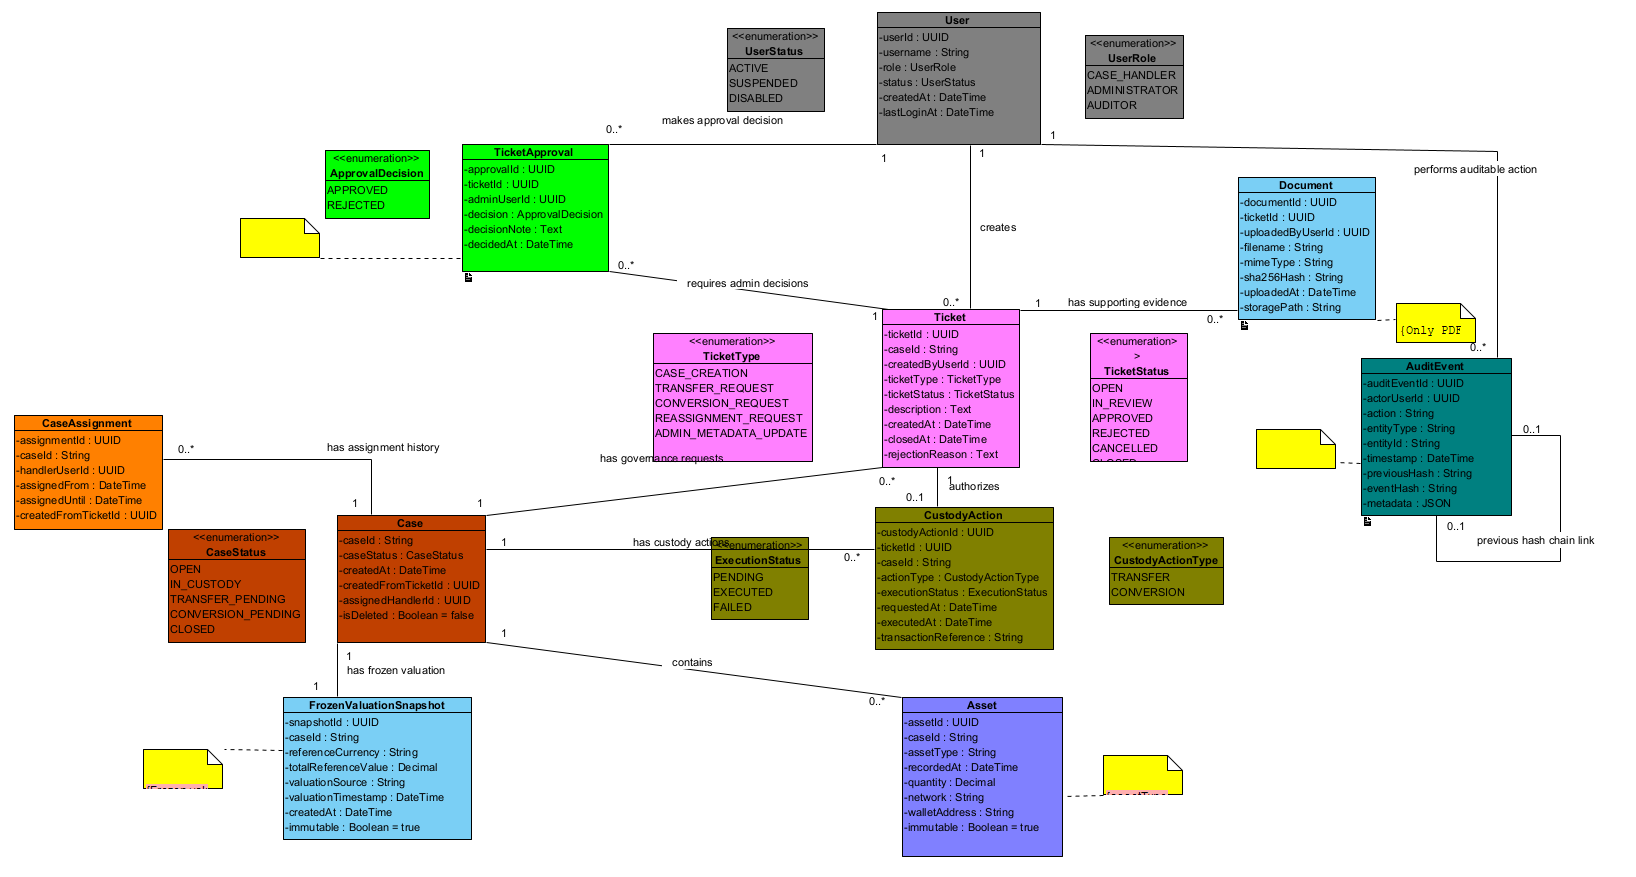
\includegraphics[width=1\linewidth]{figure19.png}
    \caption{Domain class diagram of the SCFCA core data structures.}
    \label{fig:figure19.png}
\end{figure}

Governance operations are represented through the \textit{Ticket} entity. Tickets provide
the controlled mechanism for requesting custody actions, reassignment, conversion,
transfer, or administrative metadata updates. The model deliberately separates the actor
who creates a ticket from the administrators who review it. This separation supports the
principle that sensitive custody operations must not be performed directly or informally,
but must pass through a traceable approval workflow.

The \textit{TicketApproval} entity captures administrator decisions linked to a ticket.
This class is necessary because the approval rule requires two distinct administrative
approvals before execution of custody-impacting actions. Storing approvals as separate
records makes it possible to verify who approved or rejected a request, when the decision
was made, and what decision note was provided. It also prevents the approval process
from being reduced to a simple status field, which would be weaker from an audit and
accountability perspective.

Supporting evidence is represented through the \textit{Document} entity. Documents are
linked to tickets rather than stored as isolated files, because their purpose is to justify
a specific request or governance action. Each document stores metadata such as the file
name, MIME type, uploader UserID, upload timestamp, storage path, and SHA-256 hash.
The PDF-only restriction and cryptographic hash support document integrity and allow
later verification that supporting evidence has not been silently replaced or modified.

The \textit{CustodyAction} entity represents the execution side of the workflow. It links
an approved ticket to the resulting custody operation, such as a transfer or conversion.
The action stores execution status, timestamps, and a transaction reference when
available. This design ensures that execution is not detached from authorization: every
custody action can be traced back to the ticket that originated it and to the approvals
that enabled it.

The \textit{CaseAssignment} entity preserves the history of case handler assignments.
Although the \textit{Case} entity may store the currently assigned handler, assignment
history is modeled separately to avoid losing past responsibility changes. This is important
because reassignment is a governance-relevant operation and must remain auditable over
time. The model therefore supports both operational access control and historical
accountability.

Finally, the \textit{AuditEvent} entity provides system-wide traceability. Audit events
record security-relevant actions using the actor UserID, action name, entity type, entity
identifier, timestamp, previous hash, event hash, and optional metadata. The use of
\textit{entityType} and \textit{entityId} allows audit records to refer to different domain
objects without requiring a separate direct association to every class in the diagram.
The previous-hash and event-hash fields support a tamper-evident audit chain, making
unauthorized modification of past events detectable during verification.

Overall, the domain model is not a simple persistence structure. It is an architectural
control mechanism. The selected entities and relationships encode the main security
properties of SCFCA: least-privilege access, controlled governance, immutable evidentiary
records, dual approval, traceable execution, and auditable responsibility. For this reason,
the domain model acts as a bridge between the functional requirements, the security
requirements, and the proof-of-concept implementation described in the following chapter.

In addition to the structural domain model, a Domain Security Model was developed to
show how the main SCFCA assets are protected through explicit security requirements,
security properties, misuse threats, attack paths, and mitigation mechanisms. While the
domain class diagram describes the main data entities and their relationships, the Domain
Security Model focuses on the security reasoning behind the architecture.

The model follows a simplified asset-driven structure in order to preserve readability.
Each protected asset is linked to one main security requirement, one required security
property, one representative misuse threat, one likely attack path, and one mitigation
measure. This avoids overloading the diagram while maintaining traceability between
the threat model, the formal security requirements, and the architectural controls.

\begin{figure}
    \centering
    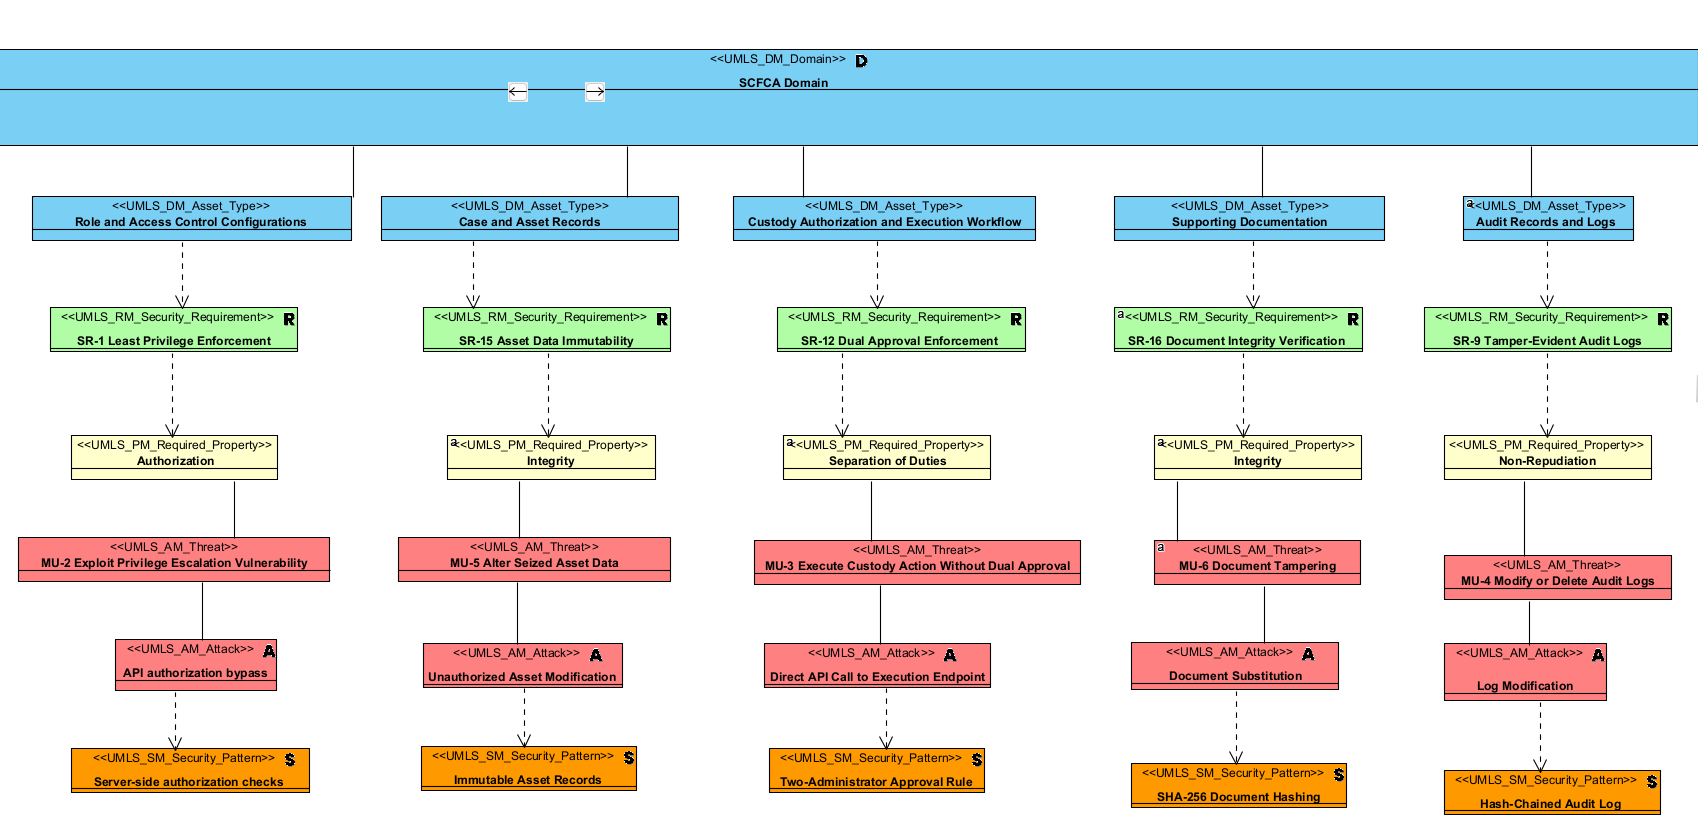
\includegraphics[width=1\linewidth]{figure17.png}
    \caption{Domain Security Model linking SCFCA assets to security requirements, threats, attacks, and mitigations.}
    \label{fig:scfca-domain-security-model}
\end{figure}



As shown in Figure~\ref{fig:scfca-domain-security-model}, the model identifies five
critical protected assets: role and access control configurations, case and asset records,
custody authorization and execution workflows, supporting documentation, and audit
records and logs. Each asset is associated with a security requirement and a security
property that directly addresses a relevant misuse scenario. For example, role and access
control configurations are protected through least-privilege enforcement against privilege
escalation, while case and asset records are protected through asset data immutability
against unauthorized asset modification.

The model also shows that governance and auditability are treated as first-class security
concerns. Custody authorization and execution workflows are protected through dual
approval enforcement, supporting documentation is protected through document integrity
verification, and audit records are protected through tamper-evident logging. In each
case, the mitigation mechanism is not an isolated technical feature, but a control derived
from the relationship between the protected asset, the threat, and the required security
property.

This Domain Security Model therefore complements the domain class diagram. The
class diagram explains how the system is structurally organized, while the security model
explains why the main domain assets require specific controls. Together, both models
support the security-by-design argument of SCFCA by linking domain entities, security
requirements, misuse threats, and mitigation mechanisms in a traceable way.

\section{Activity Workflow: Case Creation, Ticket Approval, and Custody Execution}

Figure~\ref{fig:activity-case-ticket-custody} presents the activity flow for the main
SCFCA custody governance process. The workflow begins with case creation by an
Administrator, including the upload of initial supporting documentation. The system
validates the submitted data, generates a persistent CaseID, stores the case record and
document integrity metadata, and records the creation event in the audit log.

After the case is assigned to a Case Handler, custody-impacting actions are handled
through tickets linked to the CaseID. The activity flow shows that a ticket cannot proceed
to execution after a single administrator decision. Execution is only reached after two
positive approval decisions, while any rejection path marks the ticket as rejected and
blocks the custody action.

\begin{figure}[H]
    \centering
    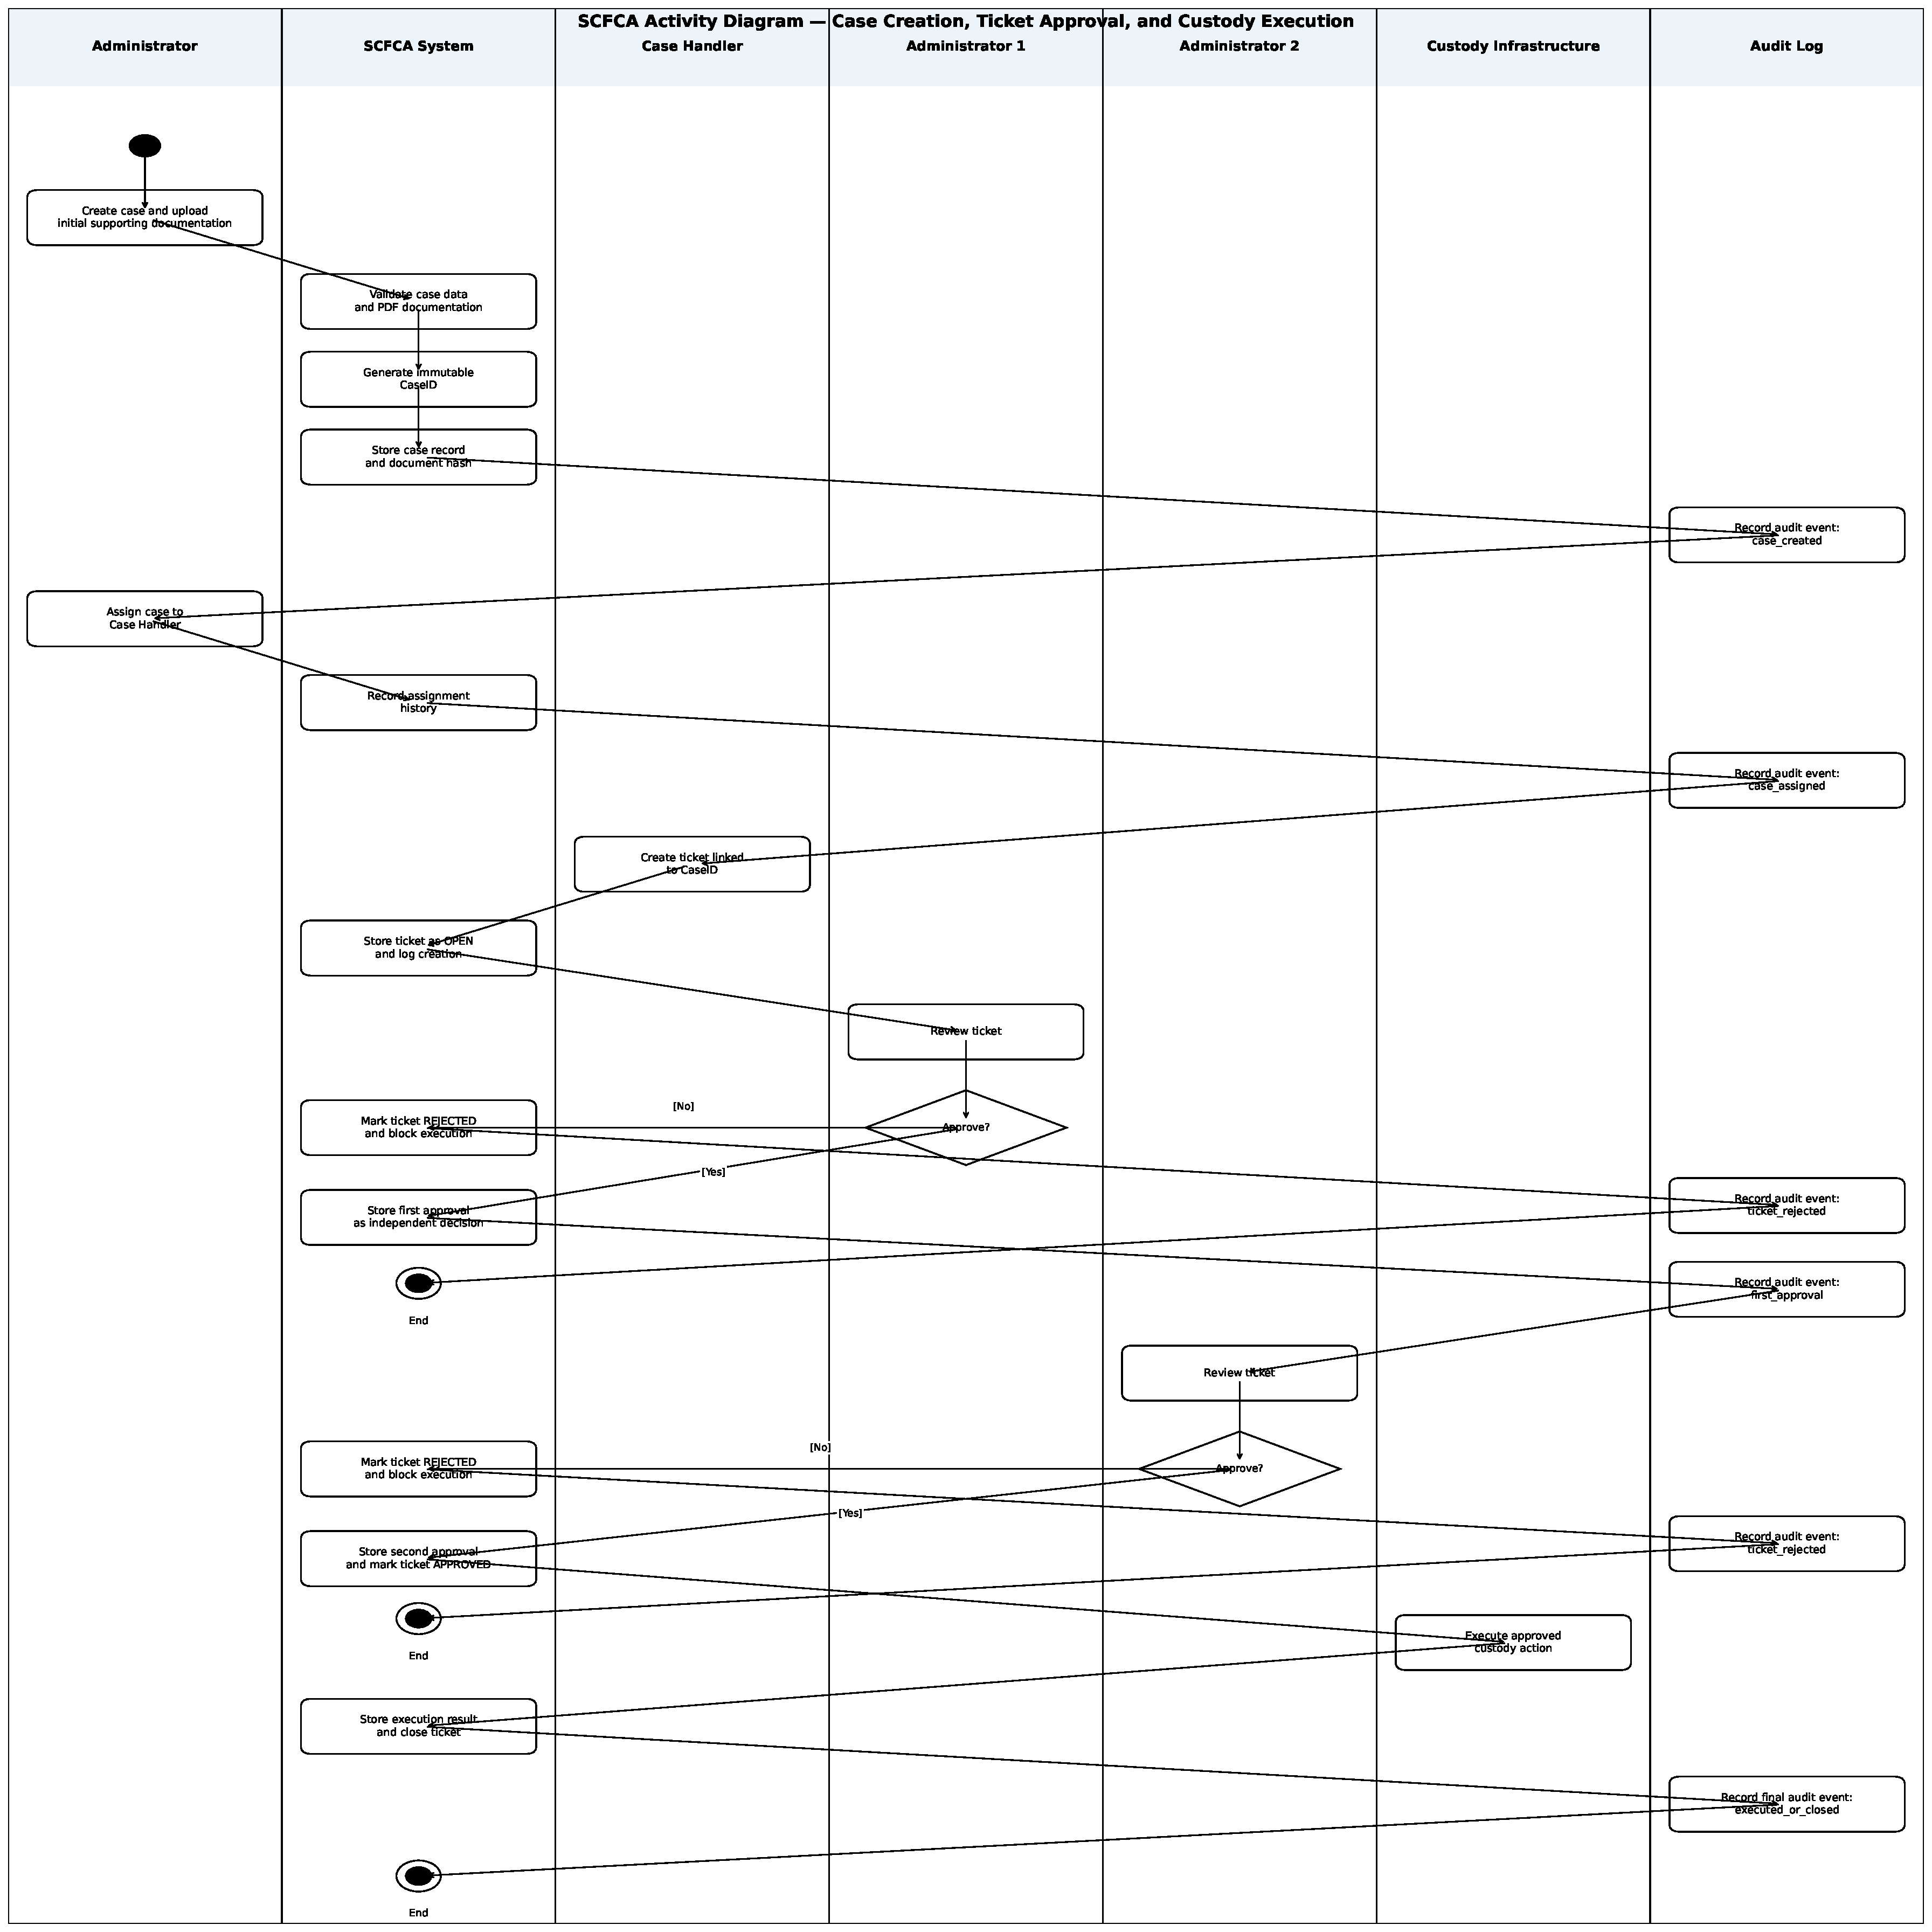
\includegraphics[width=1\linewidth]{scfca_activity_diagram_case_ticket_custody.pdf}
    \caption{Activity diagram for case creation, ticket approval, and custody execution in SCFCA.}
    \label{fig:activity-case-ticket-custody}
\end{figure}

\FloatBarrier

\section{Key Workflow Sequence: Dual Approval and Custody Execution}
\label{sec:dual-approval-sequence}

The dual-approval custody workflow is represented through three sequence-diagram
fragments for readability. The full workflow is too wide to be presented as a single
figure without losing legibility. Therefore, the sequence is divided into ticket creation
and first approval, the normal approval and execution path, and the rejection alternative.
Together, these fragments describe the complete runtime behaviour of the custody
approval process.



\begin{figure}[H]
    \centering
    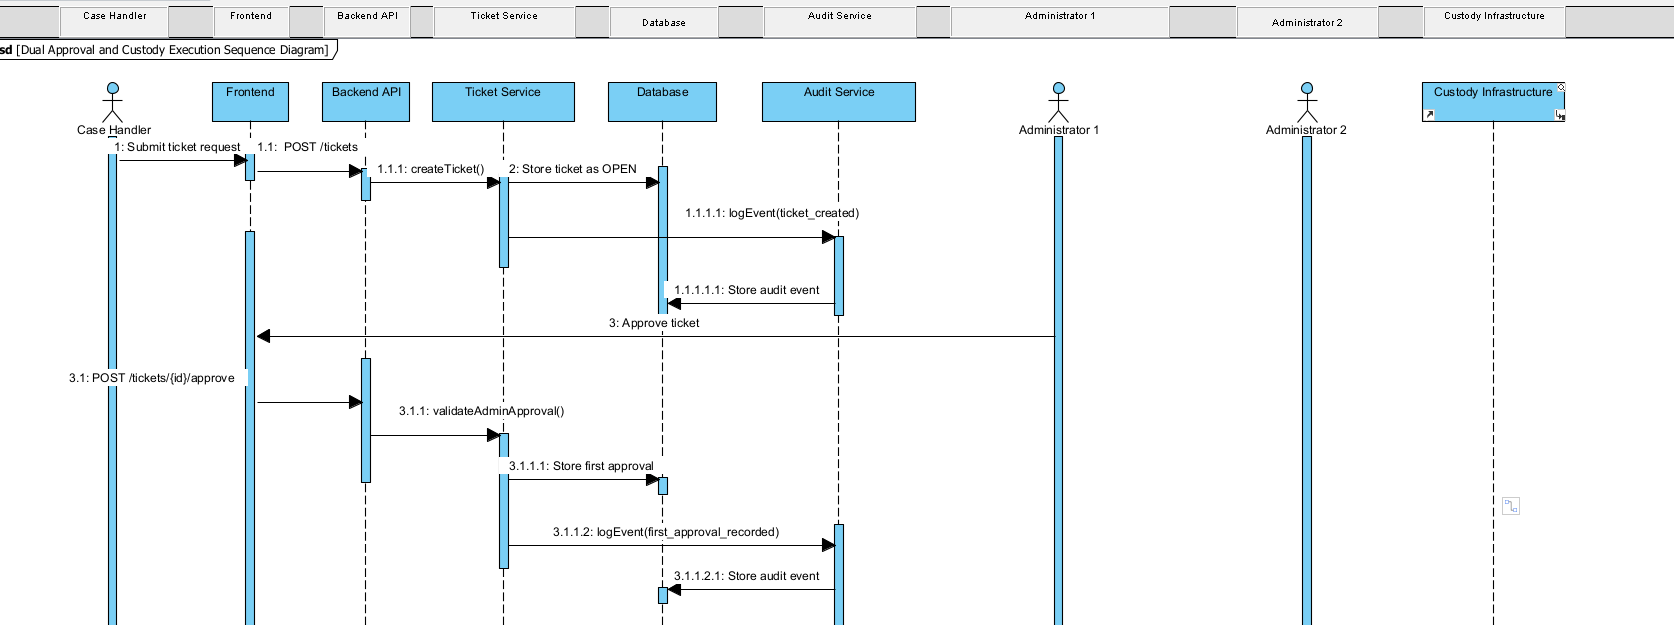
\includegraphics[width=1\linewidth]{figure20.png}
    \caption{Sequence diagram fragment for ticket creation and first administrator approval.}
    \label{fig:sequence-ticket-creation-first-approval}
\end{figure}

\begin{figure}[H]
    \centering
    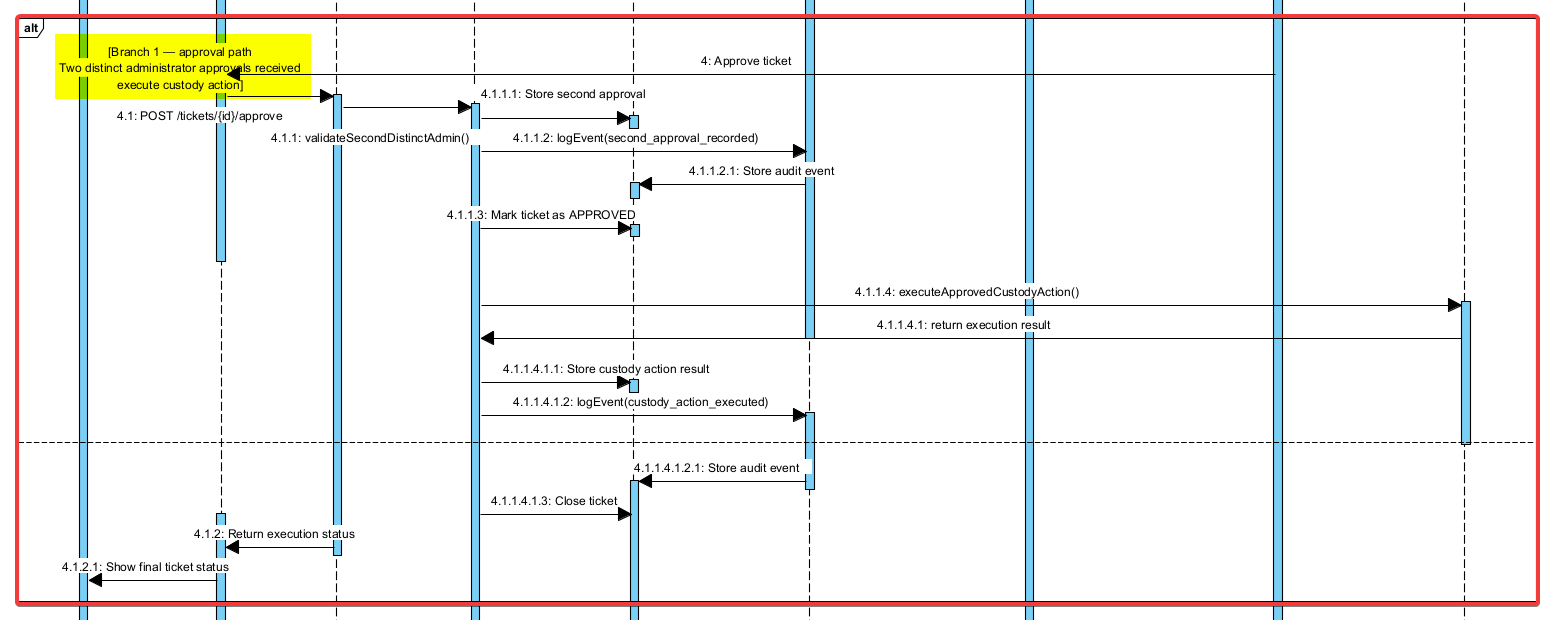
\includegraphics[width=1\linewidth]{figure21.png}
    \caption{Sequence diagram fragment for dual approval and custody execution.}
    \label{fig:sequence-approval-execution-path}
\end{figure}

\begin{figure}[H]
    \centering
    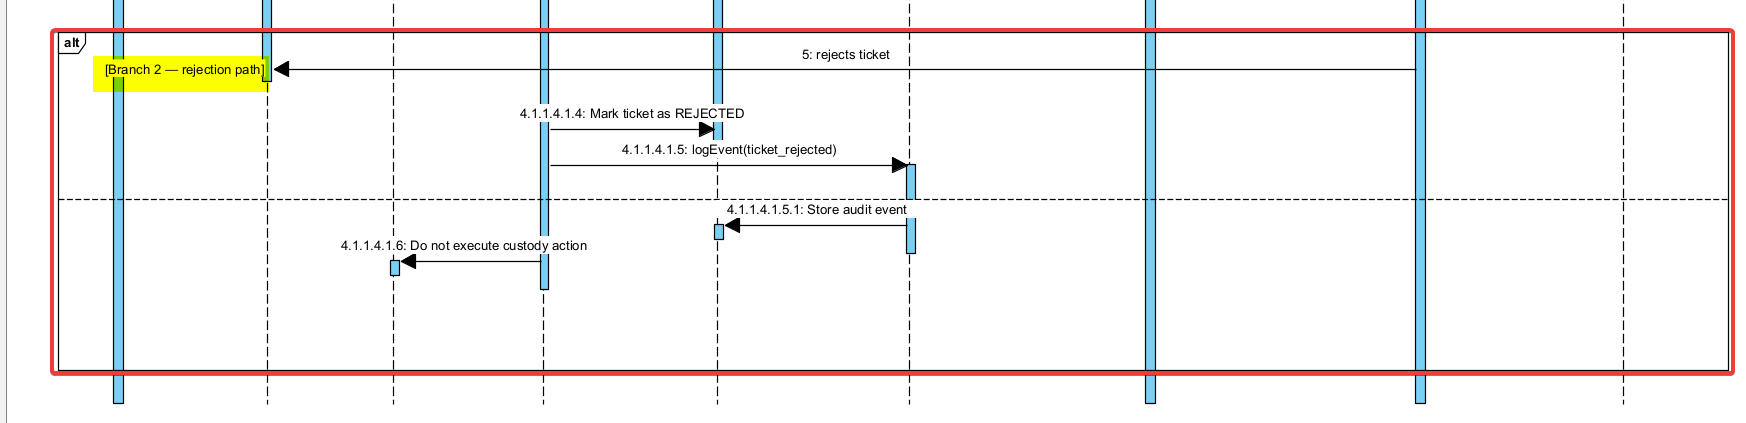
\includegraphics[width=1\linewidth]{figure22.png}
    \caption{Sequence diagram fragment for rejection handling in the custody approval workflow.}
    \label{fig:sequence-rejection-path}
\end{figure}

Figure~\ref{fig:sequence-ticket-creation-first-approval} shows the initial control point
of the workflow. The Case Handler cannot directly execute a custody operation; instead,
the request is converted into a ticket, persisted as an open workflow object, and recorded
as an audit event. This establishes the ticket as the mandatory governance object for any
later custody-impacting action.

Figure~\ref{fig:sequence-approval-execution-path} shows the normal approval path. The
first administrator approval is stored as an independent decision, but it is not sufficient
to trigger execution. The workflow only moves to execution after the second administrator
approval is validated as a distinct decision. At that point, the ticket is marked as approved,
the custody infrastructure is invoked, the execution result is stored, and the final execution
event is added to the audit trail.

Figure~\ref{fig:sequence-rejection-path} shows the negative control path. If an administrator
rejects the ticket, the system records the rejected state, stores the rejection event in the
audit log, and prevents the custody action from being executed. This branch is important
because it shows that rejection is not only a visual status change; it is a blocking governance
decision that terminates the execution path.

Together, the three sequence fragments show how the SCFCA workflow prevents direct
execution, preserves administrator decisions as separate records, and ensures that both
successful and rejected outcomes leave auditable evidence. The sequence model therefore
makes the runtime enforcement of the custody governance workflow explicit.

\section{Chapter Summary}
\label{sec:requirements-and-design-summary}

This chapter defined the requirements and design models that guide the SCFCA framework.
It identified the main institutional actors, specified the functional, security, and
non-functional requirements, and translated the core custody governance concepts into
domain, workflow, and interaction models.

The resulting models establish the design baseline for the proof-of-concept implementation.
In particular, the chapter defines how cases are created, how custody-related requests are
processed through tickets, how dual-administrator approval is enforced, how rejected
requests are blocked, and how audit evidence is generated throughout the workflow.

The following chapter builds on this design baseline by describing how the SCFCA proof of
concept was implemented and how the defined requirements were reflected in the prototype.



% =====================================================
\chapter{Implementation, Validation, and Proof of Concept}
\label{ch:implementation-validation-poc}

\section{Development Model, Environment, and Tooling}

The Secure Custody Framework for Cryptocurrency Assets (SCFCA) was implemented as a thesis-oriented proof of concept designed to validate the main architectural and security controls defined in the previous chapters. The implementation follows an iterative and incremental development model. The project was first stabilized around its base backend, frontend, database, and repository structure, and was then progressively strengthened through automated testing, Docker-based execution, GitLab CI/CD validation, security scanning, and evidence artifact generation.

The purpose of the proof of concept is to demonstrate that the central security properties of the SCFCA architecture can be translated into executable software. In particular, the implementation validates backend-enforced role-based access control, case-assignment visibility boundaries, ticket-based governance, administrator approval workflows, document integrity metadata, auditability, and reproducible DevSecOps evidence generation.

The current implementation is structured as a web application composed of the following elements:

\begin{itemize}
    \item a \textbf{FastAPI backend}, responsible for authentication, authorization, workflow enforcement, document metadata, audit events, report export, and hash verification;
    \item a \textbf{React/Vite frontend}, providing the user-facing interface for regular users, administrators, and auditors;
    \item a \textbf{PostgreSQL database}, storing users, cases, assignments, assets, valuation snapshots, tickets, approvals, documents, and audit events;
    \item a \textbf{Docker Compose runtime}, used to execute the backend, frontend, and database services in a reproducible local environment;
    \item a \textbf{GitLab CI/CD pipeline}, used to validate the repository, execute tests, build the frontend, validate container configuration, run security scanners, and retain evidence artifacts.
\end{itemize}

This implementation model reflects the two technical dimensions of the thesis. The first dimension is the secure custody governance model: the system must enforce separation of duties, restricted visibility, approval workflows, and auditability. The second dimension is the secure software engineering model: the repository must provide evidence that the system can be tested, built, scanned, and reproduced in a controlled way. This is aligned with DevOps and DevSecOps principles, where validation, automation, and feedback are integrated into the software lifecycle rather than treated as final manual activities~\cite{Kim2016,Vehent2018}.

\begin{figure}[htbp]
    \centering
    \fbox{
    \begin{minipage}{0.92\textwidth}
        \centering
        \vspace{1.2cm}
        Placeholder for implementation architecture figure.\\
        Suggested figure: React/Vite frontend, FastAPI backend, PostgreSQL database,
        Docker Compose runtime, GitLab CI/CD pipeline, and generated evidence artifacts.
        \vspace{1.2cm}
    \end{minipage}
    }
    \caption{Implementation architecture of the SCFCA proof of concept.}
    \label{fig:scfca-implementation-architecture}
\end{figure}

\section{Implemented Prototype Architecture}


The proof of concept is organized as a modular client-server application. The frontend handles interaction and presentation, while the backend remains the security-critical control point. This distinction is essential: role checks, workflow restrictions, document hashing, audit generation, and report access are enforced by backend logic rather than by client-side interface restrictions.

At a high level, the implemented prototype contains the following layers:

\begin{itemize}
    \item \textbf{Presentation layer:} React/Vite frontend for role-aware navigation and workflow interaction.
    \item \textbf{API layer:} FastAPI endpoints exposing authentication, case, ticket, document, audit, health, and internal communication functionality.
    \item \textbf{Security enforcement layer:} backend dependencies and middleware for session validation, RBAC checks, CSRF protection, and role-restricted endpoints.
    \item \textbf{Persistence layer:} PostgreSQL-backed domain records for cases, assets, documents, tickets, approvals, assignments, and audit events.
    \item \textbf{Audit and integrity layer:} audit event recording, hash-chain fields, document hash metadata, auditor report export, and hash verification.
    \item \textbf{DevSecOps evidence layer:} GitLab CI/CD jobs and retained artifacts generated by tests, builds, scanners, and report converters.
\end{itemize}

This structure supports the architectural claim made in Chapter~\ref{ch:system-architecture}: SCFCA is not only a set of requirements, but a software architecture where security controls are embedded in workflow logic, domain records, and validation evidence.

\subsection{Backend Structure}

The backend is implemented in Python using FastAPI. It exposes API routes for the main system areas: authentication, cases, tickets, documents, audit, health checks, and internal communication. The backend is the primary enforcement point for the proof of concept.

Authentication is implemented through a signed session cookie named \texttt{scfca\_session}. The session payload contains the authenticated username and role, and it is protected with an HMAC signature derived from the configured secret key. This prevents the frontend from arbitrarily declaring a different role or identity without server-side validation. State-changing requests are protected with a CSRF token mechanism based on the \texttt{scfca\_csrf} cookie and the \texttt{x-csrf-token} request header.

Role-based access control is enforced through backend dependencies. Protected endpoints require the authenticated principal to hold an allowed role before the requested operation is processed. This supports the least-privilege requirement by ensuring that authorization is checked on the server side and not left to the frontend.

The backend also implements the workflow restrictions required by SCFCA. Regular users can create custody workflow tickets only for cases assigned to them. Administrators can view all tickets and approve or reject them, but they cannot initiate regular custody workflow tickets. Auditors are restricted to audit metadata, report export, and hash-verification functionality.

\subsection{Frontend Structure}

The frontend is implemented using React, TypeScript, and Vite. Its role is to provide a clear operational interface for the different institutional roles. The frontend supports login, dashboards, case views, ticket workflows, document metadata, audit review, report export, and hash-verification interactions.

The frontend is intentionally not treated as a trusted security boundary. It may hide or show interface elements according to the authenticated role, but it does not decide whether an action is authorized. All security-relevant decisions are delegated to backend endpoints. This is important because a malicious or manipulated client could otherwise bypass frontend restrictions by sending direct HTTP requests.

The role-aware interface remains useful for operational clarity. Regular users, administrators, and auditors interact with the same system through different views that reflect their responsibilities. This supports the non-functional requirement for role-based interface clarity and reduces the likelihood of accidental misuse during demonstration and validation.

\subsection{Database and Persistence Layer}

The current proof of concept uses PostgreSQL as its persistence backend. The database stores the main domain entities required by the SCFCA workflow, including users, cases, case assignments, assets, frozen valuation snapshots, tickets, ticket approvals, document metadata, and audit events.

The use of PostgreSQL moves the project beyond a purely in-memory demonstration. Seeded records remain available across backend restarts, and role-specific visibility can be validated against persistent state. This strengthens the credibility of the proof of concept because access-control behavior can be demonstrated against the same underlying dataset from different user roles.

The repository includes a deterministic seed script for demonstration and validation. The seeded dataset includes the regular users \texttt{alice}, \texttt{mark}, and \texttt{john}, the administrators \texttt{bob} and \texttt{eve}, and the auditor \texttt{carol}. The current seeded dataset assigns cases to regular users and includes shared-case behavior, assets, documents, tickets, and audit events. This makes it possible to demonstrate concrete scenarios such as:

\begin{itemize}
    \item a regular user seeing only assigned cases;
    \item two assigned users seeing a shared case;
    \item administrators seeing all cases and tickets;
    \item administrators approving or rejecting custody workflow tickets;
    \item the auditor reviewing audit metadata, exporting reports, and verifying hashes.
\end{itemize}

This data policy also supports privacy and reproducibility. The prototype uses synthetic or seeded demonstration data only, not real judicial or investigative records.

\subsection{Docker-Based Execution}

The current repository supports Docker Compose execution for the local application stack. The Compose configuration defines three main services: PostgreSQL, backend, and frontend. This provides a reproducible runtime that reduces dependence on the developer's host environment.

The backend container runs the FastAPI application with Uvicorn. The frontend container runs the Vite development server for the proof-of-concept interface. The PostgreSQL container provides the database used by the backend. Health checks are defined for the database and backend services so that service readiness can be validated during local and CI execution.

Container hardening is included at the Docker and Docker Compose level. The backend and frontend application containers run as non-root users. The Compose configuration uses \texttt{no-new-privileges}, drops Linux capabilities for the application containers, and configures the backend container with a read-only filesystem and a temporary writable \texttt{/tmp} mount. These controls demonstrate that container security is considered as part of the PoC execution model.

\begin{figure}[htbp]
    \centering
    \fbox{
    \begin{minipage}{0.92\textwidth}
        \centering
        \vspace{1.2cm}
        Placeholder for Docker Compose architecture figure.\\
        Suggested figure: PostgreSQL service, backend service, frontend service,
        ports 5432/8000/5173, health checks, and hardening controls.
        \vspace{1.2cm}
    \end{minipage}
    }
    \caption{Docker Compose execution model for the SCFCA proof of concept.}
    \label{fig:scfca-docker-compose-model}
\end{figure}

\section{Implementation of Core Security Logic}

The implementation focuses on the controls that are most important to the thesis: server-side authorization, assignment-based visibility, ticket governance, document integrity, auditability, and DevSecOps evidence. These controls operationalize the security requirements defined in Chapter~\ref{ch:system-architecture}.

\subsection{Authentication, Session Handling, and CSRF Protection}

The authentication flow validates demo credentials against backend-controlled data and creates a signed session cookie. The session cookie stores the authenticated username and role in signed form. A manipulated or forged cookie fails signature validation and is rejected by the backend.

For state-changing routes, the backend requires a CSRF token. The login response sets a CSRF cookie and returns the token to the client. Protected mutation endpoints require the matching \texttt{x-csrf-token} header. This prevents cookie-authenticated state changes from being accepted without the expected anti-CSRF token.

This mechanism is appropriate for the PoC because the frontend and backend operate as a browser-based application using cookie-authenticated requests. It also provides concrete implementation evidence for session traceability and protected state-changing operations.

\subsection{Server-Side Role-Based Access Control}

RBAC is enforced through backend dependencies that resolve the authenticated principal and compare the user's role against the roles allowed for each endpoint. This is a central implementation decision. If role checks were enforced only in the frontend, a malicious user could bypass them by sending direct API calls. By enforcing authorization in the backend, the PoC preserves the security boundary required by the architecture.

The implemented role behavior follows the SCFCA model:

\begin{itemize}
    \item \textbf{Regular users} can view and act only within their assigned cases.
    \item \textbf{Administrators} can view all cases and tickets, assign tickets, and approve or reject ticket requests.
    \item \textbf{Auditors} can access audit metadata, report export, and hash verification, but do not receive operational modification privileges.
\end{itemize}

This implementation directly supports least privilege, separation of duties, and restricted access to sensitive case information.

\subsection{Case Visibility and Assignment Enforcement}

Case visibility is enforced using PostgreSQL case assignments. When a regular user requests the case list, the backend filters the query according to active assignments for that username. Administrators receive a broader operational view, while auditors are directed to the audit and reporting interface instead of the case-management route.

This distinction is important because case visibility is not a simple user-interface filter. It is implemented as backend query logic. The same database can therefore produce different authorized views depending on the authenticated role and assignment state.

This behavior supports the thesis requirement that case handlers must only access details for cases assigned to them, while administrators retain governance visibility and auditors retain oversight through audit metadata rather than direct case-content access.

\subsection{Ticket Workflow and Administrator Approval}

The ticket workflow is the main governance mechanism of the SCFCA proof of concept. Regular users create custody workflow tickets linked to assigned cases. Administrators review those tickets and may approve or reject them. A single administrator decision is not treated as an informal action; it is stored as part of the workflow state and remains visible for later audit review.

The implementation stores administrator decisions as approval records rather than reducing the process to a simple visual status. This preserves evidence of who approved or rejected the request, at which stage, and when. Rejection finalizes the ticket as rejected and prevents the approval path from continuing.

The current implementation also includes a case-creation-request ticket type. In this phase, administrators may submit case creation request tickets for regular handlers, while direct case creation through a backend case-creation endpoint is not the selected implementation path. This is an implementation choice in the PoC and should be understood as part of the current workflow design.

\subsection{Document Integrity Metadata}

The document subsystem stores document metadata and SHA-256 hash values. Uploaded PDF files are hashed by the backend when received through the upload endpoint. Document records are linked to cases and include metadata such as filename, document type, case identifier, uploader, creation timestamp, and hash value.

The use of hashing supports integrity verification: a later document hash can be compared against the stored value to detect replacement or modification. This is aligned with the evidentiary nature of the SCFCA domain, where supporting documentation must remain traceable and resistant to silent tampering. The cryptographic hash mechanism is used as an integrity control, consistent with standard cryptographic practice~\cite{Aumasson2021}.

\subsection{Audit Trail and Tamper-Evident Traceability}

Auditability is implemented as a first-class part of the backend. Security-relevant actions generate audit events containing metadata such as actor, role, action, entity type, entity identifier, timestamp, source/session information where available, previous hash, and current hash-chain value.

The previous-hash and hash-chain fields create tamper-evident linkage between events. The objective is not to claim that the database itself is physically immutable. Instead, the PoC demonstrates that audit records can be chained so that unauthorized modification of past entries becomes detectable during verification. This supports the thesis objective of preserving traceability, accountability, and non-repudiation in custody workflows.

The auditor-facing functionality includes filtered audit review, JSON report export, HTML report export, and hash verification. The hash verification endpoint can determine whether a submitted hash corresponds to a known document hash or audit-event hash. This allows an auditor to verify integrity using safe metadata without requiring access to confidential case narratives or document contents.

\begin{figure}[htbp]
    \centering
    \fbox{
    \begin{minipage}{0.92\textwidth}
        \centering
        \vspace{1.2cm}
        Placeholder for audit evidence screenshot.\\
        Suggested figure: Auditor dashboard, HTML audit report, or hash verification result.
        \vspace{1.2cm}
    \end{minipage}
    }
    \caption{Auditor-facing audit evidence and hash verification in the SCFCA proof of concept.}
    \label{fig:scfca-audit-evidence-placeholder}
\end{figure}

\section{DevSecOps Evidence Layer}

The implementation includes a DevSecOps evidence layer built around GitLab CI/CD. This layer is not separate from the proof of concept; it supports the thesis argument that secure custody systems should be developed and validated through repeatable engineering evidence, not only through design claims.

The GitLab pipeline is organized around validation, testing, build, and security stages. It validates the backend, frontend, Docker configuration, dependencies, static code properties, secrets exposure, container images, configuration files, and dynamic application behavior. Security jobs are intentionally non-blocking at this stage. Their purpose is to preserve evidence, expose findings, and support triage, not to claim a mature production release gate.

\subsection{GitLab CI/CD Pipeline}

The GitLab CI/CD pipeline provides automated validation of the repository. The main non-security jobs include:

\begin{itemize}
    \item backend compilation and application import checks;
    \item Docker Compose configuration validation;
    \item PostgreSQL-backed backend tests using \texttt{pytest};
    \item frontend production build verification using \texttt{npm run build}.
\end{itemize}

The backend test job uses a PostgreSQL service, waits for database readiness, runs the demo seed script, and then executes the test suite. This is important because it verifies backend behavior in a CI environment using a database-backed execution path, not only in the developer's local environment.

\begin{figure}[htbp]
    \centering
    \fbox{
    \begin{minipage}{0.92\textwidth}
        \centering
        \vspace{1.2cm}
        Placeholder for GitLab CI/CD pipeline screenshot.\\
        Suggested figure: GitLab pipeline showing validate, test, build, and security stages.
        \vspace{1.2cm}
    \end{minipage}
    }
    \caption{GitLab CI/CD pipeline stages used to validate the SCFCA proof of concept.}
    \label{fig:scfca-gitlab-pipeline-placeholder}
\end{figure}

\subsection{Software Composition Analysis}

Software Composition Analysis is included to provide visibility into dependency risk. The backend dependency audit uses \texttt{pip-audit} against \texttt{backend/requirements.txt}. The frontend dependency audit uses \texttt{npm audit} against the frontend npm dependency tree.

Both jobs produce machine-readable JSON artifacts. These artifacts allow dependency findings to be reviewed, preserved, and compared over time. The pipeline also converts scanner outputs into HTML summaries where supported by the reporting script, making the results easier to inspect during thesis review.

This does not eliminate dependency risk. It provides repeatable visibility, which is the correct claim for this proof of concept.

\subsection{SAST and Secret Scanning}

Static Application Security Testing is performed through two tools. Bandit scans the Python backend for common Python security issues. Semgrep performs broader static analysis using a default ruleset. These tools provide source-level evidence that the codebase has been scanned for common classes of insecure patterns.

Secret scanning is performed with Gitleaks. The purpose of this job is to detect committed secrets or sensitive values that should not be present in the repository. This is especially relevant because the project includes Docker, CI/CD, backend configuration, and demo credentials. Demo accounts are intentionally documented for validation, but real secrets must not be committed.

The SAST and secret scanning jobs are evidence jobs. Their output requires human review and triage before any claim can be made about the relevance or severity of specific findings.

\subsection{Container and Configuration Scanning}

Container image scanning is performed with Trivy. The pipeline builds backend and frontend Docker images and scans them for known vulnerabilities. This connects the implementation with the Docker execution model and provides evidence about the security state of the built images.

Infrastructure-as-Code and configuration scanning is performed with Checkov. The Checkov job scans Dockerfiles, YAML files, and GitLab CI configuration. This is relevant because insecure configuration can weaken the system even when application logic is correct. In the SCFCA context, Docker hardening, CI/CD configuration, and container execution are part of the software trust boundary.

\subsection{DAST with OWASP ZAP}

Dynamic Application Security Testing is performed using the OWASP ZAP baseline scan. The pipeline starts the PoC stack through Docker Compose, waits for the backend health endpoint, waits for the frontend to become reachable, and then runs ZAP against the frontend target.

The ZAP job produces JSON, HTML, and Markdown artifacts. This is useful because it provides both machine-readable and human-readable DAST evidence. The current ZAP baseline scan is unauthenticated, so it should be interpreted as baseline dynamic evidence rather than exhaustive application security testing.

\subsection{Human-Readable HTML Evidence Reports}

The repository includes a script for converting scanner JSON outputs into human-readable HTML summaries. The purpose of this phase is to make security evidence usable for thesis review, professor inspection, and screenshots, while keeping JSON artifacts for traceability and future automation.

The HTML report approach is important because raw JSON artifacts are useful for machines but difficult to inspect during an academic defense. HTML summaries make the evidence more readable without discarding the original scanner outputs.

\begin{figure}[htbp]
    \centering
    \fbox{
    \begin{minipage}{0.92\textwidth}
        \centering
        \vspace{1.2cm}
        Placeholder for generated HTML security evidence screenshot.\\
        Suggested figure: Bandit, Semgrep, Trivy, Checkov, pip-audit, npm audit,
        Gitleaks, or ZAP HTML report.
        \vspace{1.2cm}
    \end{minipage}
    }
    \caption{Human-readable security evidence report generated from CI scanner output.}
    \label{fig:scfca-html-security-report-placeholder}
\end{figure}

\section{Testing and Validation Evidence}

The validation strategy verifies that the proof of concept behaves consistently with the architecture and requirements defined earlier in the thesis. The objective is not broad feature completeness, but confirmation that the core institutional workflows and security constraints are enforceable.

The validation combines automated tests, CI/CD execution, scanner evidence, Docker-based reproducibility, and planned manual validation. This combination is appropriate for a security-oriented proof of concept because security claims must be supported by executable behavior and reviewable evidence.

\subsection{Automated Functional and Security Tests}

The repository includes automated tests covering workflow behavior, model behavior, security hardening, and malformed input handling. The tests are executed in GitLab CI against a PostgreSQL-backed environment after the demo seed script has populated the database.

The automated tests support the following validation claims:

\begin{itemize}
    \item the backend application imports and compiles correctly;
    \item authentication and role mismatch behavior are controlled;
    \item regular users are restricted to assigned-case visibility;
    \item administrators can perform ticket review actions;
    \item auditors are restricted to audit, report, and hash-verification behavior;
    \item CSRF protection blocks unsafe state-changing requests without the expected token;
    \item malformed document names, ticket descriptions, and case identifiers produce controlled client errors rather than unhandled server errors;
    \item the frontend can be built successfully;
    \item the Docker Compose configuration can be validated by CI.
\end{itemize}

These tests provide implementation evidence that the modeled controls were not only described in the thesis, but translated into backend behavior.

\subsection{Hypothesis-Based Robustness Tests}

The repository includes Hypothesis-based security input tests. These tests generate malformed inputs for selected backend paths, including invalid document names, ticket descriptions, and case identifiers. The objective is to verify that malformed inputs produce controlled responses such as \texttt{400} or \texttt{404}, rather than unexpected \texttt{500} server errors.

This type of testing does not replace deeper fuzzing or formal verification. However, it adds useful robustness evidence because it checks input-handling behavior across generated cases rather than only hand-written examples.

\subsection{Manual Validation Checklist}

Manual validation is planned as a complementary evidence layer. Automated tests and scanners are necessary, but they do not fully replace human review of role behavior, workflow logic, and generated artifacts. The manual validation checklist should document the following checks:

\begin{itemize}
    \item login as \texttt{alice}, \texttt{mark}, \texttt{john}, \texttt{bob}, \texttt{eve}, and \texttt{carol};
    \item regular-user visibility for assigned cases;
    \item shared-case visibility for the Mark/John shared case;
    \item administrator visibility across cases and tickets;
    \item ticket approval and rejection behavior;
    \item document upload and SHA-256 hash recording;
    \item auditor access to audit metadata;
    \item JSON and HTML audit report export;
    \item document hash and audit hash verification;
    \item GitLab CI/CD artifact inspection;
    \item security report review for SCA, SAST, secret scanning, Trivy, Checkov, and ZAP.
\end{itemize}

\begin{figure}[htbp]
    \centering
    \fbox{
    \begin{minipage}{0.92\textwidth}
        \centering
        \vspace{1.2cm}
        Placeholder for manual validation checklist screenshot or table.\\
        Suggested figure: checklist showing login, RBAC, ticket workflow, audit report,
        hash verification, and CI artifact review.
        \vspace{1.2cm}
    \end{minipage}
    }
    \caption{Manual validation checklist for SCFCA proof-of-concept behavior.}
    \label{fig:scfca-manual-validation-placeholder}
\end{figure}

\subsection{Final Reproducibility Check}

After the implementation and DevSecOps phases are complete, a final reproducibility check is planned. The final repository will be copied or uploaded into a new blank GitLab project, and the full pipeline will be executed from scratch.

This step is intended to verify that the CI/CD configuration, Docker setup, automated tests, security scanning jobs, and evidence artifacts work in a clean GitLab environment without depending on local machine state or hidden configuration from the original project. This strengthens the thesis evidence because it demonstrates that the repository is reproducible as an independent GitLab CI/CD project.

\section{Analysis of Results}

The implementation and validation results support the central argument of the thesis: a governance-driven custody architecture can be translated into a working software system that enforces role separation, restricted visibility, ticket-based control, auditability, document integrity metadata, and repeatable security evidence generation.

The first relevant result is that security decisions are enforced in the backend. The frontend supports usability and workflow clarity, but authorization decisions are made server-side. This directly supports the least-privilege and separation-of-duties requirements.

The second result is that case visibility is assignment-based. Regular users do not receive the same operational view as administrators. This validates the architectural requirement that case handlers must only access assigned cases while administrators retain governance-level visibility and auditors operate through audit metadata.

The third result is that the ticket workflow acts as a governance control. Custody-impacting requests are represented as tickets, administrator decisions are recorded, and rejected tickets are prevented from continuing through the approval path. This supports the dual-control and execution-traceability logic defined in the architecture.

The fourth result is that auditability is implemented as a concrete subsystem. Audit events are stored with metadata and hash-chain fields, and auditor-facing endpoints support report export and hash verification. This demonstrates that auditability is not merely described as a requirement, but implemented as a reviewable mechanism.

The fifth result is that the repository now includes a stronger DevSecOps evidence layer. The GitLab pipeline validates the backend, frontend, Docker configuration, dependencies, static analysis, secret exposure, container images, configuration files, and DAST behavior. JSON artifacts support traceability, while HTML reports support human review.

These results do not need to be exaggerated. The value of the proof of concept is that it demonstrates architectural feasibility and evidence-based validation for the SCFCA model.

\section{Scope Boundaries}

The current proof of concept demonstrates the feasibility and coherence of the SCFCA architecture within an academic and controlled validation scope.

The implementation validates the governance, access-control, auditability, document integrity, Docker execution, and DevSecOps evidence aspects of SCFCA. It does not execute real blockchain transactions, manage real private keys, integrate production HSM or MPC infrastructure, or provide a certified institutional custody service.

Some security requirements are implemented directly in the current repository, such as backend RBAC, CSRF protection, signed session cookies, case-assignment visibility, document hashing, audit event recording, hash-chain metadata, report export, Docker hardening, and CI/CD evidence generation. Other controls remain architectural or future-hardening items, especially production-grade cryptographic custody, full external log anchoring, production secret management, authenticated DAST, runtime monitoring, signed provenance, and long-term durable binary evidence storage.

The CI/CD security jobs are evidence-generating and visibility-first. They produce useful scanner output and human-readable reports, but they are not claimed as production release gates. Their findings require human triage and selected remediation. This is appropriate for the thesis because the goal is to demonstrate DevSecOps-oriented validation evidence, not to claim that all vulnerabilities have been eliminated.

\section{Chapter Summary}

This chapter described the implementation, validation, and proof-of-concept evidence for SCFCA. The prototype combines a FastAPI backend, React/Vite frontend, PostgreSQL persistence, Docker Compose execution, backend-enforced security controls, audit/hash verification, and GitLab CI/CD evidence generation.

The implementation demonstrates that the core SCFCA controls can be operationalized: regular users are restricted by case assignment, administrators participate in controlled ticket approval and rejection, auditors receive read-only audit/report/hash-verification capabilities, documents are associated with SHA-256 integrity metadata, and security-relevant actions are recorded in a tamper-evident audit trail.

The chapter also described the DevSecOps evidence layer added around the project. The GitLab pipeline validates the backend, frontend, Docker configuration, dependencies, static analysis, secret scanning, container images, configuration files, and DAST behavior, while preserving JSON and HTML artifacts for review.

The next chapter concludes the thesis by summarizing the achieved objectives, the controlled scope boundaries of the proof of concept, and future work directions such as hardware-backed custody integration, stronger runtime monitoring, authenticated DAST, signed provenance, and deeper institutional deployment hardening.

% =====================================================
\chapter{Conclusions and Future Work}
\section{Achievement of Objectives}
The results of this thesis indicate that the main objectives defined at the beginning of the work have been achieved within the intended academic scope.

The first objective was to analyze the technical characteristics and security risks associated with institutional cryptocurrency custody. This objective was addressed through the study of custody models, governance challenges, security threats, and regulatory context. The analysis showed that the custody of confiscated cryptocurrency assets cannot be reduced to cryptographic key storage alone, but must also address governance, workflow control, accountability, and auditability in institutional environments. In this sense, the work successfully identified the central risks affecting such systems, including unauthorized access, insider abuse, privilege escalation, custody manipulation, audit tampering, and confidentiality breaches.
The second objective was to identify and model the relevant threats affecting institutional cryptocurrency custody systems. This objective was fulfilled through the misuse-case–driven threat analysis developed in the threat-modeling chapter. The work defined adversarial scenarios involving both external attackers and malicious insiders, mapped them to security goals, and linked them to explicit mitigation measures. This produced a structured traceability chain from misuse scenarios to requirements and from requirements to architectural controls.

The third objective was to define a secure custody architecture based on security-by-design principles, separation of duties, access control, and role management. This objective was achieved through the specification of the SCFCA reference architecture, including institutional actors, functional requirements, security requirements, non-functional requirements, trust boundaries, and governance mechanisms such as dual approval, restricted execution authority, immutable asset facts, and pseudonymous identity representation. The architecture also evolved to include secure software architecture considerations, dependency trust, and software supply chain governance, thereby strengthening its alignment with modern DevSecOps and secure software design principles.

The fourth objective was to design a logging and auditing approach capable of guaranteeing traceability, accountability, and non-repudiation. This objective was achieved both conceptually and at the proof-of-concept level. The proposed framework treats auditability as a first-class security property and not as a secondary administrative feature. The PoC demonstrates that meaningful system events can be recorded, linked to authenticated identities, and protected with tamper-evident mechanisms that improve evidentiary reliability.

Finally, the work sought to align the proposed framework with European cybersecurity, governance, and risk-management principles while keeping it applicable to institutional contexts. This objective was addressed through the inclusion of regulatory context, resilience-oriented design choices, and the integration of DevSecOps concepts such as software supply chain visibility, monitoring, and certifiability-oriented evidence generation.

Taken together, these results show that the thesis has achieved its main purpose: to design and justify a secure, auditable, and institution-oriented technical framework for the custody and management of confiscated cryptocurrency assets. The contribution is not a finished industrial product, but a traceable reference architecture supported by a coherent proof of concept that validates the feasibility of its most critical controls.

\section{Limitations of the Prototype}
Despite the positive results obtained, the current proof of concept has clear limitations that define the boundary of the contribution and must be acknowledged explicitly.

First, the prototype does not implement live blockchain interaction or real transaction execution against production cryptocurrency networks. As a result, the custody-execution aspect of the system remains at the level of controlled workflow simulation rather than operational digital asset transfer. This is an intentional scoping decision consistent with the academic focus of the thesis, but it means that the PoC does not demonstrate end-to-end production custody under real network conditions.

Second, the prototype does not integrate physical Hardware Security Modules (HSMs), secure enclaves, or equivalent dedicated cryptographic hardware. Instead, it validates the governance and control envelope that would surround such components in a real institutional deployment. This is sufficient for demonstrating the architecture’s logic, but it does not substitute for production-grade key ceremonies, secure device integration, hardware-backed signing, or formal assurance of cryptographic key custody.

Third, the implementation is not intended to represent a production-ready operational platform. Although it includes important security controls such as server-side RBAC, dual approval, tamper-evident logging, MFA for privileged roles, re-authentication for sensitive actions, and containerized execution support, it does not yet cover the full industrial requirements of a real institutional custody service. Areas such as high-availability deployment, hardened secret management, full incident-response automation, infrastructure hardening, and large-scale operational monitoring would require substantial further development.

Fourth, the DevSecOps and software supply chain aspects of the prototype remain partially demonstrative. The repository structure and pipeline configuration are aligned with practices such as SAST, dependency scanning, secret detection, container scanning, and SBOM-centered transparency, but these mechanisms are not yet fully activated and operationalized as a mature continuous-assurance system. Accordingly, the thesis can claim architectural alignment with those practices, but not full industrial implementation of them.

Fifth, the validation strategy remains limited to architectural correctness, feasibility demonstration, and workflow-oriented security evidence. It does not include formal verification of cryptographic protocols, independent penetration testing by external evaluators, empirical usability studies, or long-term production deployment assessment. These omissions are not accidental; they reflect the intended scope of the thesis as a design-oriented and security-engineering contribution rather than a full operational certification exercise.

For these reasons, the prototype should be interpreted as evidence of feasibility and architectural coherence, not as a complete institutional custody product. Its value lies in demonstrating that the proposed governance-driven architecture can be implemented in software and can enforce the most critical controls required for secure institutional cryptocurrency custody.

\section{Future Lines of Research}

The results of this thesis open several relevant directions for future work, both from the perspective of institutional cryptocurrency custody and from the perspective of secure software engineering.

A first and immediate line of future work concerns the integration of real cryptographic custody infrastructure. The current proof of concept validates the governance and control logic surrounding sensitive custody actions, but it does not execute real blockchain transactions or interact with dedicated cryptographic hardware. A natural next step would therefore be the integration of Hardware Security Modules (HSMs) or equivalent secure signing components capable of supporting production-grade key generation, key storage, and transaction authorization. This would make it possible to extend the current architecture from a feasibility prototype toward a more operational custody platform.

A second important direction concerns more advanced custody models based on distributed cryptographic control. In particular, Multi-Party Computation (MPC) offers a promising path for future evolution because it can support decentralized signing workflows without concentrating full key material in a single device or location. For institutional environments, this may strengthen resilience against insider abuse, reduce single points of compromise, and provide alternative operational models for high-assurance transfer approval.

A third line of future work concerns the expansion of the framework toward stronger software supply chain assurance. While this thesis already incorporates dependency trust, software composition visibility, and DevSecOps-oriented validation at a conceptual level, future versions of SCFCA could implement these practices more fully. This includes automatic SBOM generation for every build, continuous Software Composition Analysis (SCA), stricter CI/CD security gates, artifact signing, preserved security-scan evidence per release, and stronger verification of dependency provenance. Such improvements would increase both operational security and institutional confidence in the software construction process itself.

Closely related to this is a fourth line of research focused on certifiability-by-design. The current architecture, repository organization, and traceability logic already suggest a path toward stronger audit and certification readiness. Future work could formalize this by linking requirements, code, tests, deployment records, scan results, and release artifacts into a more explicit assurance chain. This would improve the suitability of the framework for external audit, regulatory review, and high-assurance institutional adoption.

A fifth direction concerns monitoring and operational resilience in real deployment scenarios. The present work defines a security-monitoring strategy for evolving systems, but future research could validate it in a live multi-environment deployment with centralized telemetry, alert correlation, anomaly detection, and incident-response automation. This would allow the framework to move from design-oriented runtime assurance toward experimentally validated continuous operational security.

Finally, the SCFCA could be extended beyond the specific institutional and national context that motivated this thesis. Although the work was framed with particular attention to the needs of public authorities managing confiscated cryptocurrency assets, future research could adapt the framework to different legal systems, regulatory environments, and operational models. Comparative adaptation across jurisdictions would be especially valuable for understanding which parts of the architecture are universally applicable and which must be tailored to local procedural or legal constraints.

In summary, the future evolution of SCFCA should move in two complementary directions: deeper custody realism and stronger assurance maturity. On one side, this means integrating real cryptographic infrastructure, advanced signing models, and live operational workflows. On the other, it means strengthening software supply chain governance, monitoring, and certifiability. Together, these directions would help transform the present reference architecture into a more deployable and institutionally defensible custody platform.

% =====================================================
\appendix
\chapter*{Appendix A: Mapping of Thesis Requirements to Project Implementation}
\addcontentsline{toc}{chapter}{Appendix A: Mapping of Thesis Requirements to Project Implementation}

This appendix maps high-level thesis security goals to the project modules and files that implement them, answering the question: which part of the codebase addresses each architectural claim?


\begin{longtable}{|p{4cm}|p{6cm}|p{5cm}|}
\hline
\textbf{Thesis Requirement / Security Control} & \textbf{Project File(s) / Module(s) / Test(s)} & \textbf{Description / Implementation Details} \\
\hline
Secure custody of cryptocurrency assets & backend/custody/.keep (placeholder), backend/models/, backend/services/ & Custody module placeholder; models and services would implement key/custody logic in a full system \\
\hline
RBAC (Role-Based Access Control) & backend/auth/dependencies.py, backend/auth/schemas.py, backend/auth/service.py, backend/auth/routes.py & Role extraction, enforcement, and authentication logic; require\_role, require\_any\_role functions \\
\hline
Authentication \& JWT & backend/auth/jwt.py, backend/auth/routes.py, backend/auth/service.py & JWT-based authentication, token issuance, and validation \\
\hline
Dual approval / separation of duties & backend/tickets/, backend/services/tickets.py, backend/models/tickets.py, tests/test\_workflows.py & Ticket approval flow, status transitions, dual-approval logic, tested in test\_ticket\_dual\_approval\_execution... \\
\hline
Audit logging \& traceability & backend/audit/service.py, backend/audit/poc\_audit.py, backend/services/audit\_log.py, tests/test\_workflows.py & Append-only, hash-chained audit log, event recording, audit chain verification, tested in workflows \\
\hline
CSRF protection & backend/middleware/csrf.py, tests/test\_workflows.py (test\_csrf\_blocks\_unsafe\_without\_header) & Middleware for CSRF token validation, enforced for unsafe methods, tested for blocking requests without token \\
\hline
Rate limiting & backend/middleware/rate\_limit.py, backend/services/rate\_limit.py, tests/test\_security\_phase5.py & Per-IP and per-endpoint rate limiting, login throttling, tested for lockout and abuse scenarios \\
\hline
MFA (Multi-Factor Authentication) & backend/auth/mfa.py, tests/test\_security\_phase5.py & MFA setup and verification endpoints, tested for enrollment and code validation \\
\hline
Re-authentication for sensitive actions & backend/auth/reauth.py, backend/services/reauth.py, tests/test\_security\_phase5.py & Re-auth token issuance and validation, required for ticket execution, tested for enforcement \\
\hline
Asset immutability & backend/models/assets.py, tests/test\_cases\_and\_assets.py (test\_asset\_immutability\_enforced) & ORM-level enforcement of immutability, tested for attempts to modify asset quantity \\
\hline
Automated \& manual testing & tests/test\_workflows.py, tests/test\_security\_phase5.py, tests/test\_cases\_and\_assets.py, README.md (test instructions) & End-to-end and unit tests for all major workflows and security controls \\
\hline
Audit chain verification & backend/audit/service.py (verify\_chain), tests/test\_workflows.py & Hash-chained audit log, endpoint and test for verifying audit chain integrity \\
\hline
Documentation \& traceability & docs/traceability-matrix.md, docs/implementation-record.md, README.md, docs/testing-guide.md & Explicit mapping from requirements to code/tests, implementation rationale, and test instructions \\
\hline
Demo script / walkthrough & README.md (Demo Script section), tests/test\_workflows.py & Step-by-step demo and test coverage for all critical workflows and security controls \\
\hline
\end{longtable}

% =====================================================
\chapter*{Appendix B: Requirements-to-Implementation Traceability}
\addcontentsline{toc}{chapter}{Appendix B: Requirements-to-Implementation Traceability}

This appendix maps individual requirement IDs (FR, SR, MU) to their implementation locations and test evidence, answering the question: which specific requirement is covered by which file and test?

\begin{longtable}{|p{1.2cm}|p{4.5cm}|p{5cm}|p{4.3cm}|}
\hline
\textbf{Req. ID} & \textbf{Requirement Description} & \textbf{Implementation Location(s)} & \textbf{Test(s) / Evidence} \\
\hline
FR-1 & Only authorized users can access custody functions & backend/auth/, backend/middleware/, backend/services/ & tests/test\_user\_management.py, test\_workflows.py \\
\hline
FR-2 & Dual approval required for asset transfer & backend/tickets/, backend/services/tickets.py & tests/test\_workflows.py (dual approval) \\
\hline
FR-3 & All custody actions are audit-logged & backend/audit/service.py, backend/audit/poc\_audit.py & tests/test\_workflows.py (audit chain) \\
\hline
FR-4 & MFA required for privileged actions & backend/auth/mfa.py & tests/test\_security\_phase5.py (MFA) \\
\hline
FR-5 & CSRF protection enforced & backend/middleware/csrf.py & tests/test\_workflows.py (CSRF) \\
\hline
FR-6 & Rate limiting on sensitive endpoints & backend/middleware/rate\_limit.py & tests/test\_security\_phase5.py (rate limit) \\
\hline
FR-7 & Asset immutability after registration & backend/models/assets.py & tests/test\_cases\_and\_assets.py (immutability) \\
\hline
FR-8 & Re-authentication for execution & backend/auth/reauth.py & tests/test\_security\_phase5.py (reauth) \\
\hline
FR-9 & Traceability from requirements to code/tests & docs/traceability-matrix.md, README.md & test coverage, documentation \\
\hline
FR-10 & Role-based access for all API endpoints & backend/auth/dependencies.py, backend/auth/schemas.py & tests/test\_user\_management.py, test\_workflows.py \\
\hline
FR-11 & Tamper-evident audit log (hash chain) & backend/audit/service.py, backend/audit/poc\_audit.py & tests/test\_workflows.py (audit chain verification) \\
\hline
FR-12 & Ticket lifecycle: creation, approval, execution, audit & backend/tickets/, backend/services/tickets.py & tests/test\_workflows.py (ticket flow) \\
\hline
FR-13 & Document upload and integrity verification & backend/documents/, backend/services/documents.py & tests/test\_documents\_and\_reports.py \\
\hline
FR-14 & User management: CRUD, RBAC, MFA & backend/users/, backend/auth/, backend/services/users.py & tests/test\_user\_management.py \\
\hline
FR-15 & Case and asset registration, assignment, and audit & backend/cases/, backend/assets/, backend/services/cases.py & tests/test\_cases\_and\_assets.py \\
\hline
FR-16 & Automated and manual test coverage for all workflows & tests/, README.md (test instructions) & 41 passing tests, demo walkthrough \\
\hline
FR-17 & Demo script for thesis defense & README.md (Demo Script section) & Step-by-step demo, test evidence \\
\hline
SR-1 & No single actor can both initiate and approve custody-impacting actions & backend/tickets/, backend/services/tickets.py & tests/test\_workflows.py (dual approval) \\
\hline
SR-2 & All privileged actions require MFA or re-auth & backend/auth/mfa.py, backend/auth/reauth.py & tests/test\_security\_phase5.py \\
\hline
SR-3 & All sensitive actions are logged and auditable & backend/audit/service.py & tests/test\_workflows.py \\
\hline
MU-1 & Unauthorized modification of protected records is denied & backend/models/assets.py, backend/services/ & tests/test\_cases\_and\_assets.py \\
\hline
MU-2 & Replay and idempotency protection for ticket execution & backend/tickets/, backend/services/tickets.py & tests/test\_workflows.py (idempotency) \\
\hline
MU-3 & Rate limiting blocks brute-force and abuse & backend/middleware/rate\_limit.py & tests/test\_security\_phase5.py \\
\hline
\end{longtable}

\chapter*{Appendix C: Granular Security Requirements Mapping}
\addcontentsline{toc}{chapter}{Appendix C: Granular Security Requirements Mapping}

This appendix maps security mechanisms to the specific endpoints, classes, and methods that enforce them, answering the question: how exactly is each security control implemented at the code level?

\begin{longtable}{|p{3cm}|p{4cm}|p{5cm}|p{4cm}|}
\hline
\textbf{Security Requirement} & \textbf{Feature / Endpoint / Function} & \textbf{File(s) / Class / Method} & \textbf{Test(s) / Evidence} \\
\hline
RBAC & Role checks on all endpoints, require\_role, require\_any\_role & backend/auth/dependencies.py: require\_role, require\_any\_role & tests/test\_user\_management.py, test\_workflows.py \\
\hline
Authentication (JWT) & Login, token issuance, token validation & backend/auth/routes.py: /login, /me, /logout & tests/test\_user\_management.py, test\_workflows.py \\
\hline
Session Management & JWT in HttpOnly cookie, session expiration & backend/auth/routes.py, backend/auth/jwt.py & tests/test\_workflows.py \\
\hline
Password Security & Password hashing, password check & backend/auth/service.py: authenticate\_user, hash\_password & tests/test\_user\_management.py \\
\hline
Dual Approval & Ticket approval workflow, status transitions & backend/tickets/routes.py: /tickets/\{id\}/approve & tests/test\_workflows.py (dual approval) \\
\hline
Audit Logging & log\_event, list\_events, verify\_chain & backend/audit/service.py: log\_event, list\_events, verify\_chain & tests/test\_workflows.py (audit chain) \\
\hline
MFA & MFA setup, verification, enforcement & backend/auth/mfa.py: /auth/mfa/setup, /auth/mfa/verify & tests/test\_security\_phase5.py (MFA) \\
\hline
CSRF Protection & CSRF token set, checked on unsafe methods & backend/middleware/csrf.py: CSRFMiddleware & tests/test\_workflows.py (CSRF) \\
\hline
Rate Limiting & Per-IP and per-endpoint limits, login throttling & backend/middleware/rate\_limit.py: RateLimitMiddleware & tests/test\_security\_phase5.py (rate limit) \\
\hline
Asset Immutability & Prevent asset modification after registration & backend/models/assets.py: Asset model, ORM listener & tests/test\_cases\_and\_assets.py (immutability) \\
\hline
Re-authentication & Re-auth token issuance, required for execution & backend/auth/reauth.py: /auth/reauth, backend/services/reauth.py & tests/test\_security\_phase5.py (reauth) \\
\hline
Privilege Escalation Prevention & Role checks, explicit allow-lists & backend/auth/dependencies.py, backend/auth/schemas.py & tests/test\_user\_management.py, test\_workflows.py \\
\hline
Input Validation & Pydantic models, FastAPI validation & backend/api/, backend/models/ & All test suites \\
\hline
Error Handling & Controlled error messages, no sensitive info in responses & backend/services/, backend/api/ & tests/test\_workflows.py \\
\hline
Logging \& Monitoring & Audit logs, event recording, log integrity & backend/audit/service.py, backend/audit/poc\_audit.py & tests/test\_workflows.py (audit log) \\
\hline
Supply Chain Security & Dockerfile, requirements.txt, CI/CD config & Dockerfile, requirements.txt, .github/workflows/ (if present) & Project structure, README.md \\
\hline
Data Minimization \& Privacy & Minimal data in logs, privacy in monitoring & backend/services/, backend/audit/ & tests/test\_workflows.py \\
\hline
\end{longtable}


% =====================================================
\printbibliography



\end{document}
